\documentclass[10pt]{article}



\usepackage[export]{adjustbox}
\usepackage{algorithm}
\usepackage[noend]{algpseudocode}
\usepackage{amsmath}
\usepackage{amssymb}
\usepackage{amsthm}
\usepackage{caption}
\usepackage{cite}
\usepackage{enumitem}
\usepackage{fullpage}
\usepackage{graphicx}
\usepackage{hyperref}
\usepackage{ifthen}
\usepackage{mathtools}
\usepackage{multirow}
\usepackage{stackrel}
\usepackage{subcaption}
\usepackage{wrapfig}
\usepackage{mleftright}
\mleftright % make \left & \right behave like \mleft & \mright

%\ProvidesPackage{commands-tam}
\usepackage{amsfonts}
%\usepackage[labelfont=bf]{caption}

\providecommand{\prob}{\mathrm{Pr}}
\newcommand{\calT}{\mathcal{T}}

% Blackboard Bold Sets
\newcommand{\N}{\mathbb{N}}
\newcommand{\Z}{\mathbb{Z}}
\newcommand{\Q}{\mathbb{Q}}
\newcommand{\R}{\mathbb{R}}

% easy way to write sets
% use setr if the contents to the right of the | are bigger
% use setl if the contents to the left of the | are bigger
\newcommand{\setr}[2]{\left\{\ #1 \ \left|\ #2 \right. \ \right\}}
\newcommand{\setl}[2]{\left\{\ \left. #1 \ \right|\ #2 \ \right\}}

% TAM stuff
\newcommand{\norm}[1]{\left\Vert#1\right\Vert}
\newcommand{\set}[1]{\left\{#1\right\}}
\newcommand{\Real}{\mathbb R}
\newcommand{\eps}{\varepsilon}
\providecommand{\To}{\longrightarrow}
\newcommand{\BX}{\mathbf{B}(X)}
\newcommand{\A}{\mathcal{A}}
\providecommand{\func}[3]{#1 : #2 \rightarrow #3 }
\newcommand{\pfunc}[3]{#1 : #2 \dashrightarrow #3 }
\newcommand{\bigpair[2]}{\left(#1, #2\right)}
%\newcommand{\color}{{\rm col}}
\newcommand{\lab}{{\rm label}}
\newcommand{\colorf}[1]{\color(#1)}
\newcommand{\strength}{{\rm str}}
\newcommand{\strengthf}[1]{\strength(#1)}
\newcommand{\bbval}[1]{\left[\!\left[ #1 \right] \! \right]}
\newcommand{\dom}{{\rm dom} \;}
\newcommand{\asmb}{\mathcal{A}}
\newcommand{\asmbt}[2]{\asmb^{#1}_{#2}}
\newcommand{\asmbtt}{\mathcal{A}^\tau_T}
\newcommand{\ste}[2]{#1 \mapsto #2}
\newcommand{\frontier}[3]{{\partial}^{#1}_{#2}{#3}}
\newcommand{\frontiert}[1]{\partial^{\tau}{#1}}
\newcommand{\frontiertt}[1]{\frontier{\tau}{t}{#1}}
\newcommand{\frontiertx}[2]{{\partial}^{\tau}_{#1}{#2}}
\newcommand{\frontiertau}[1]{{\partial}^{\tau}{#1}}
\newcommand{\arrowstett}[2]{#1 \xrightarrow[\tau,T]{1} #2}
\newcommand{\arrowste}[2]{#1 \stackrel{1}{\To} #2}
\newcommand{\arrowtett}[2]{#1 \xrightarrow[\tau,T]{} #2}
\newcommand{\res}[1]{\textrm{res}(#1)}
\newcommand{\termasm}[1]{\mathcal{A}_{\Box}[\mathcal{#1}]}
\newcommand{\prodasm}[1]{\mathcal{A}[\mathcal{#1}]}
\newcommand{\fgg}[1]{fgg^\#_{#1}}
\newcommand{\ftdepth}[2]{\textrm{ft-depth}_{#1}\left(#2\right)}
\newcommand{\str}[1][*]{\textrm{str}_{#1}}
\newcommand{\col}[1]{\textrm{col}_{#1}}
\newcommand{\tmblank}{\llcorner \negthinspace\lrcorner}
\newcommand{\fullgridgraph}{G^\mathrm{f}}\newcommand{\bindinggraph}{G^\mathrm{b}}


\DeclarePairedDelimiter\ceil{\lceil}{\rceil}
\DeclarePairedDelimiter\floor{\lfloor}{\rfloor}

\DeclarePairedDelimiter\bigo{O\left(}{\right)}
\newtheorem{theorem}{Theorem}
\newtheorem{lemma}{Lemma}

\begin{document}


\section{Definitions}
\label{sec:prelims}

\newcommand{\dr}{\mathcal{DR}}

\begin{flalign*}
    \text{Let }  m & = \text{base of the counter} & \\
               MSR & = \text{ most signifcant digit region } \\
             c_{0} & = \text{starting value of counter}  \\
                 d & = \ceil*{\log_m({c_0})},              \text{ number of digits per row }  \\
              \dr  & = \ceil*{\frac{d}{3}},                \text{ digit regions per row }           \\
             c_{f} & = m^{d} - 1,                          \text{ final value of the counter} \\
        c_{\Delta} & = c_f - c_0,                          \text{ number of rows }            \\
                 l & = \ceil{\log m} + 2, \text{ bits needed to represent each digit plus 2 for MSR and MSD} & \\
\dr_{height} & = 3 \cdot (l + 30),                   \text{ height of a row }           \\
                 h & = c_{\Delta} \cdot \dr_{height}, \text{ height of constuction without roof tiles }   \\
\end{flalign*}


In order to determine the number of digits per row, given some value $k$, let $R = k \mod 6$. There are 3 distinct cases to consider.

\begin{itemize}[label={--}]

    \item if $0 \leq R \leq 1$, then $\setl{d\in\mathbb{N}}{3 \text{ divides } d}$ \\
        MSR $\gets$ 3 digits

    \item if $2 \leq R \leq 3$, then $\setl{d\in\mathbb{N}}{3 \text{ divides } d - 1}$ \\
        MSR $\gets$ 1 digit

    \item if $4 \leq R \leq 5$, then $\setl{d\in\mathbb{N}}{3 \text{ divides } d - 2}$ \\
        MSR $\gets$ 2 digits

\end{itemize}

In order to account for odd values of $k$, when $k$ is odd, one vertical filler tile is added to increase the width
of the rectangle. O(1)



$\dr_{1st}$ = $3l + 90$ + 1

$\dr_{general}$ = $3l + 90$

$\dr_{last}$ = $3l + 75$

Let $n$ be the number of counter unit rows, then
\begin{flalign*}
    h & = (n - 1) \cdot \dr_{general} + \dr_{1st} + \dr_{last}  & \\
      & = (m^d - 1) (3l + 90) + 6l + 166  \\
\end{flalign*}

$m = \ceil*{\left(\frac{N}{93}\right)^{\frac{1}{d}}}$

\begin{flalign*}
    N & = 93 \left(\frac{N}{93}\right) = 93 \left(\left(\frac{N}{93}\right)^{\frac{1}{d}}\right)^d \leq 93 \ceil*{\left(\frac{N}{93}\right)^{\frac{1}{d}}}^d & \\
      & = 93 (m^d - 1) \leq 3lm^d + 90m^d \leq 3lm^d + 90m^d + 3l + 91  \\
      & = (m^d - 1) (3l + 90) + 6l + 166  \\
\end{flalign*}



% \section{Seed counter}
% \begin{figure}
%     \centering
%     \begin{subfigure}[t]{0.2\textwidth}
%         \centering
%         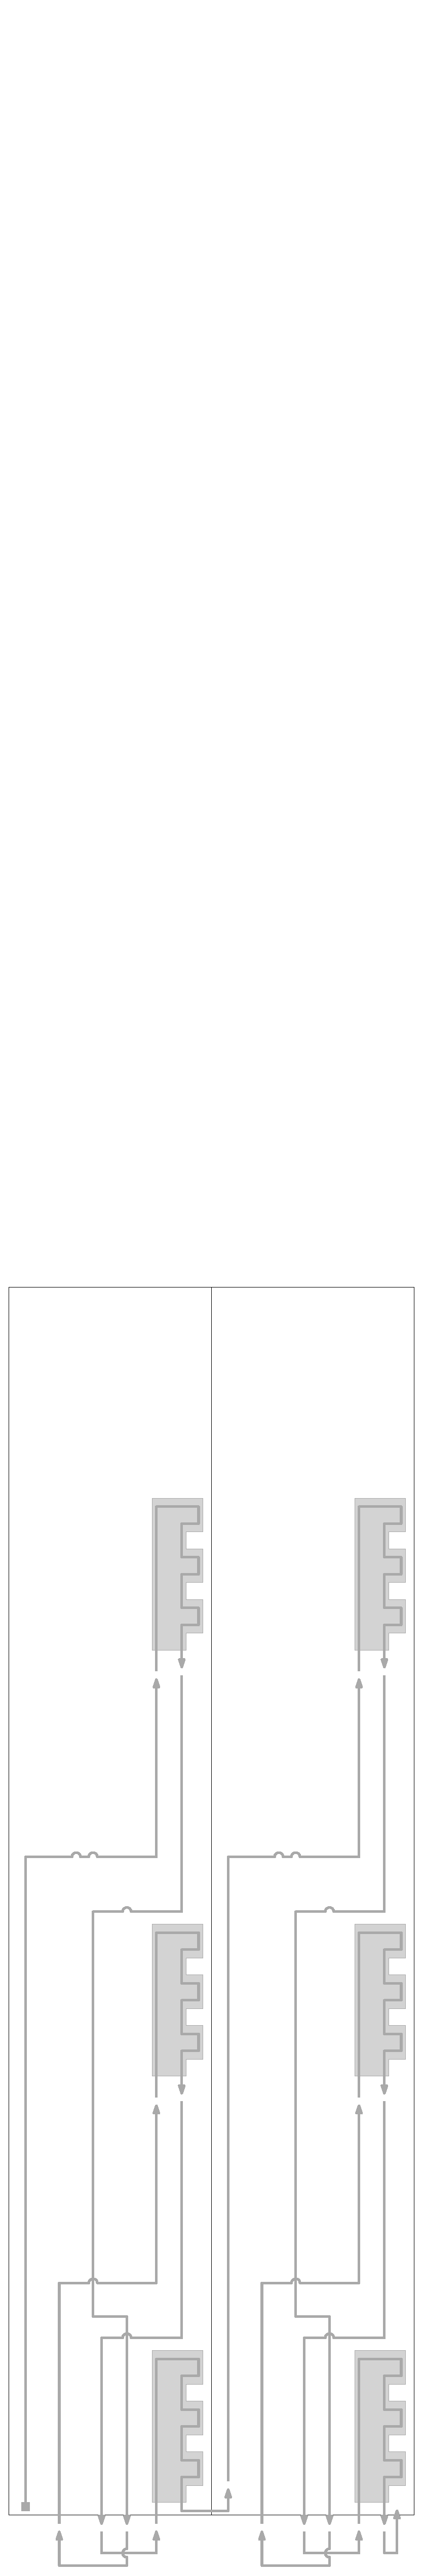
\includegraphics[width=0.6in]{counter_read_start_seed_case3_middle_level}
%         \caption{\label{fig:counter_read_start_seed_case3_middle_level} A ``clean'' counter row, before any reading has started.}
%     \end{subfigure}%
%     ~
%     \begin{subfigure}[t]{0.2\textwidth}
%         \centering
%         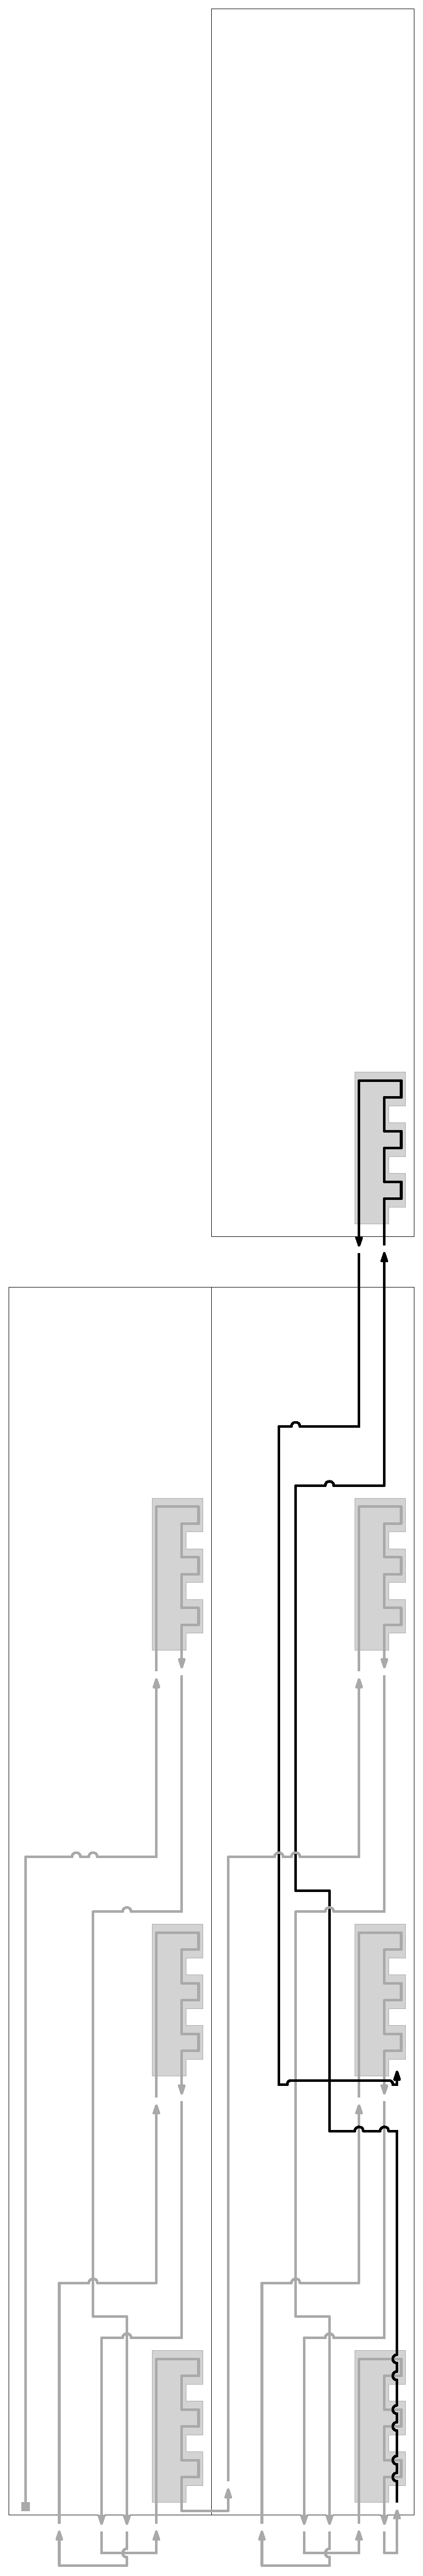
\includegraphics[width=0.6in]{counter_read_digit1_return_read_digit2_seed_case3_middle_level}
%         \caption{\label{fig:counter_read_digit1_return_read_digit2_seed_case3_middle_level} Reading digit 1, writing digit 1 in the next row, and returning to read digit 2 of the current row. }
%     \end{subfigure}%
%     ~
%     \begin{subfigure}[t]{0.2\textwidth}
%         \centering
%         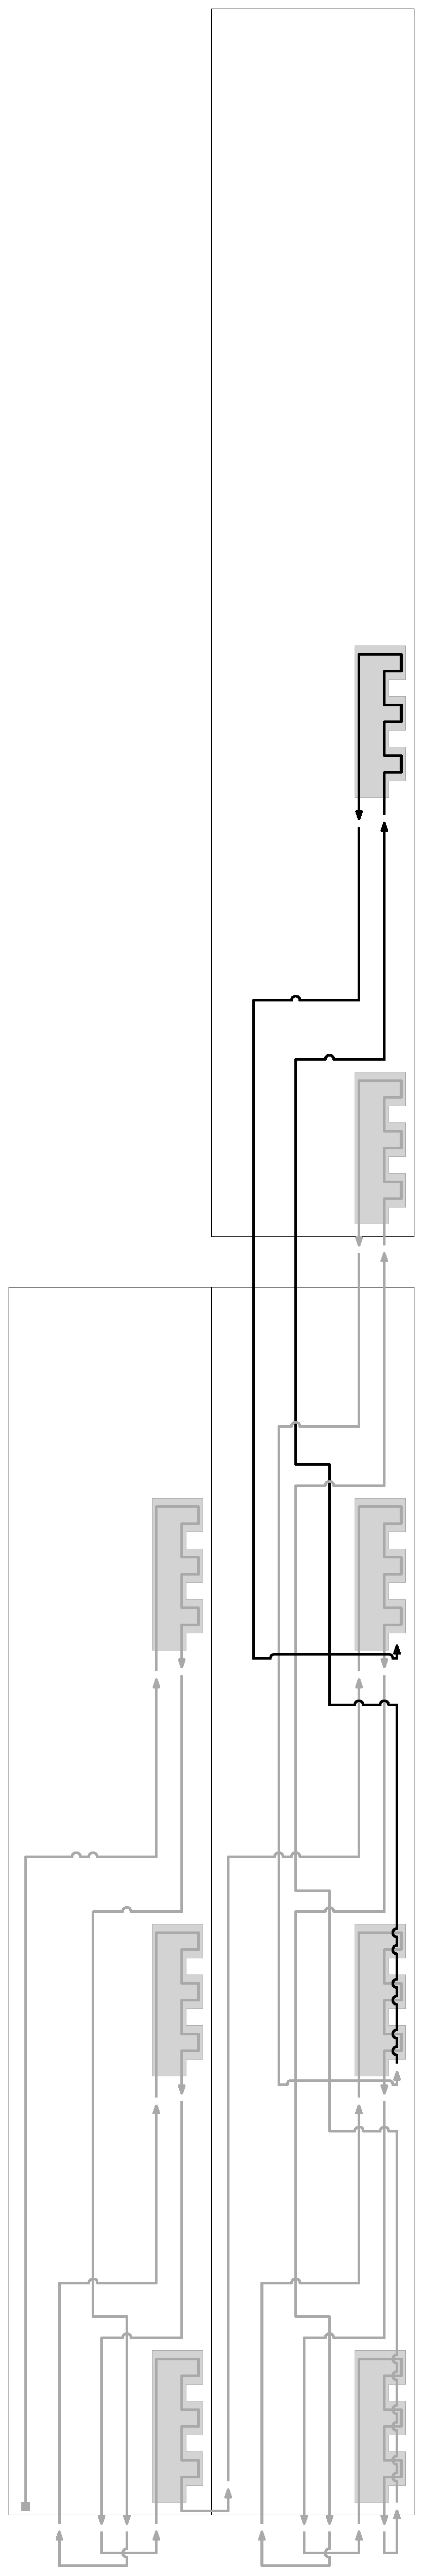
\includegraphics[width=0.6in]{counter_read_digit2_return_read_digit3_seed_case3_middle_level}
%         \caption{\label{fig:counter_read_digit2_return_read_digit3_seed_case3_middle_level} Reading digit 2, writing digit 2 in the next row, and returning to read digit 3 of the current row. }
%     \end{subfigure}%
%     ~
%     \begin{subfigure}[t]{0.2\textwidth}
%         \centering
%         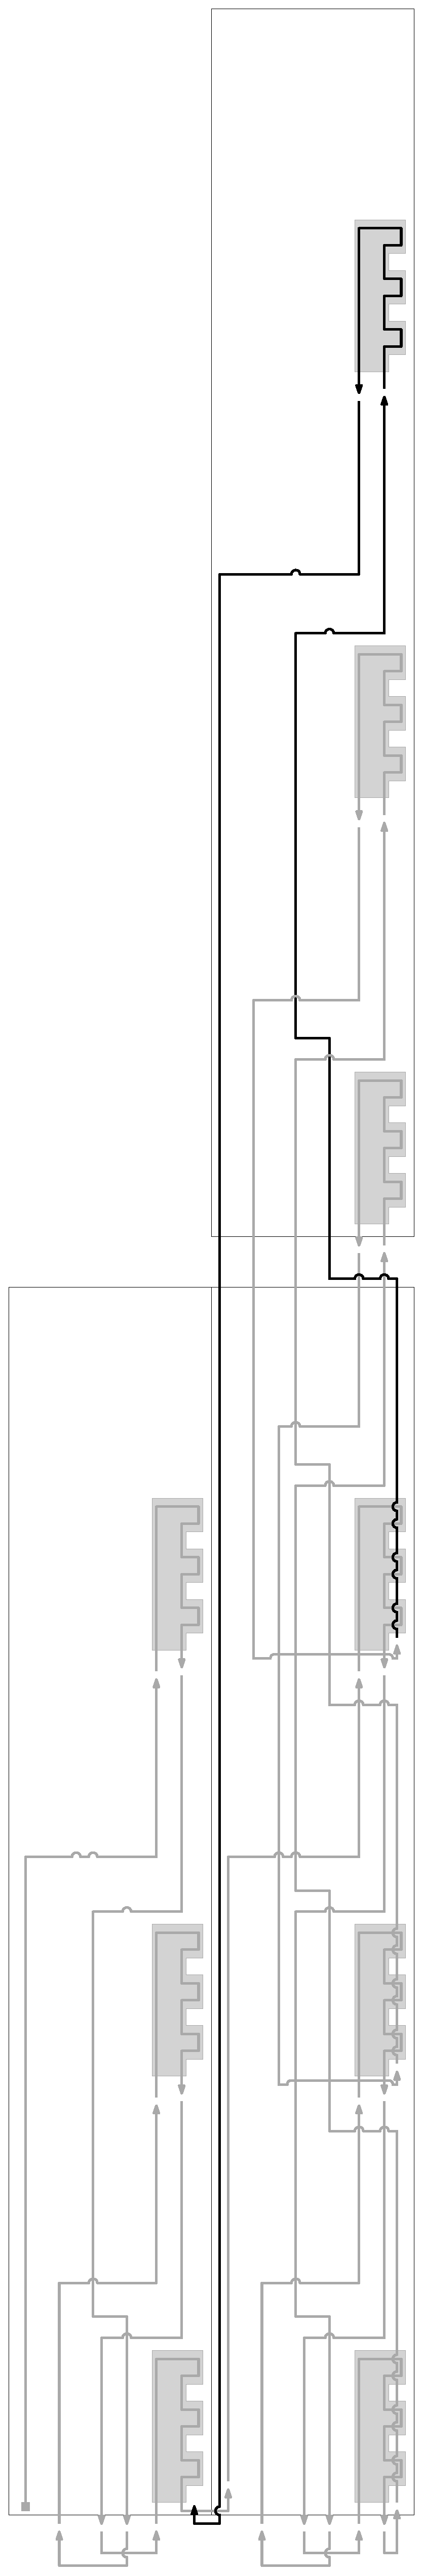
\includegraphics[width=0.6in]{counter_read_digit3_return_read_digit1_seed_case3_middle_level}
%         \caption{\label{fig:counter_read_digit3_return_read_digit1_seed_case3_middle_level} Reading digit 3, writing digit 3 in the next row, and returning to read digit 4 of the current row.}
%     \end{subfigure}%

%     \caption{\label{fig:counter_read_digit_return_read_digit_seed_case3} Progression of the counter as it reads the 3 least significant digits in one value, and writes the corresponding digits in the next row/value.}
% \end{figure}


\section{General counter}


\begin{figure}[H]
    \centering
    \begin{subfigure}[t]{0.2\textwidth}
        \centering
        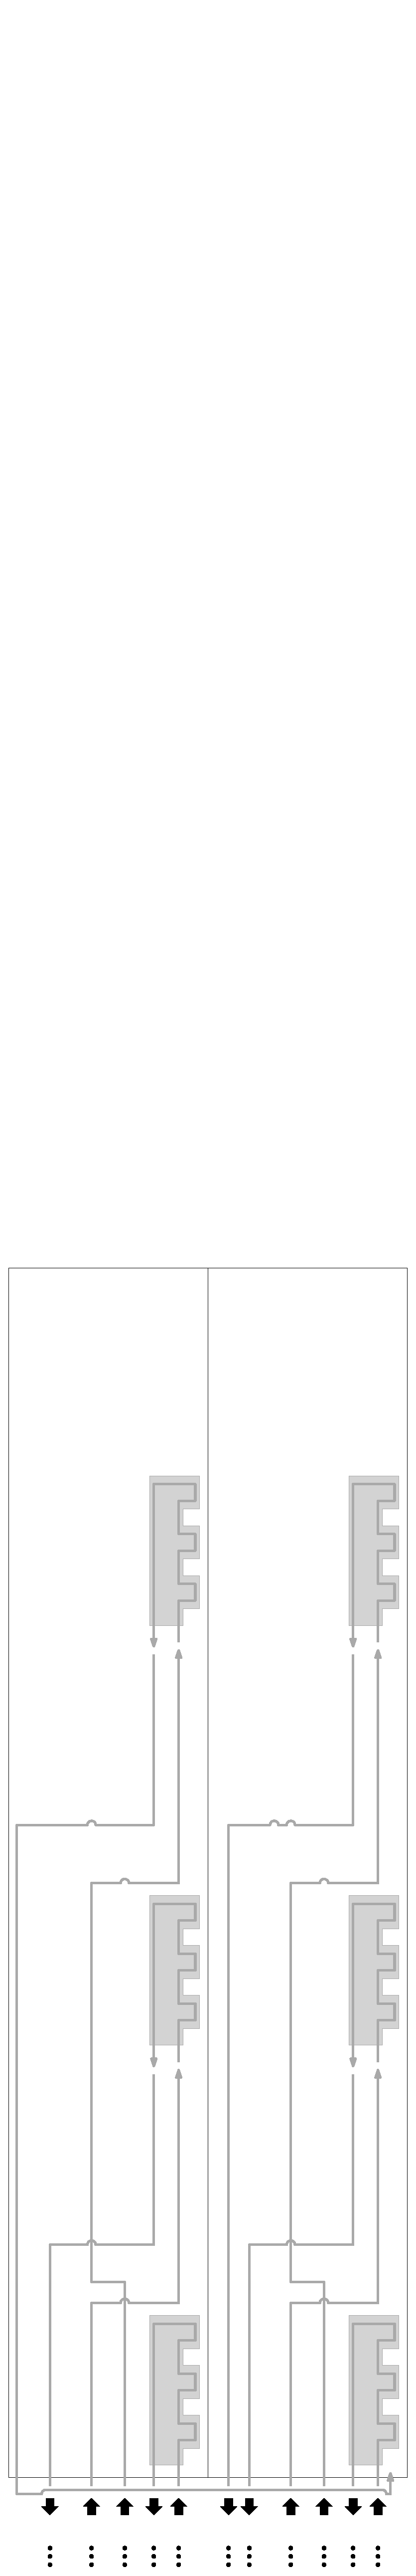
\includegraphics[width=0.6in]{counter_read_start_general_case3_middle_level}
        \caption{\label{fig:counter_read_start_general_case3_middle_level} A ``clean'' counter row, before any reading has started.}
    \end{subfigure}%
    ~
    \begin{subfigure}[t]{0.2\textwidth}
        \centering
        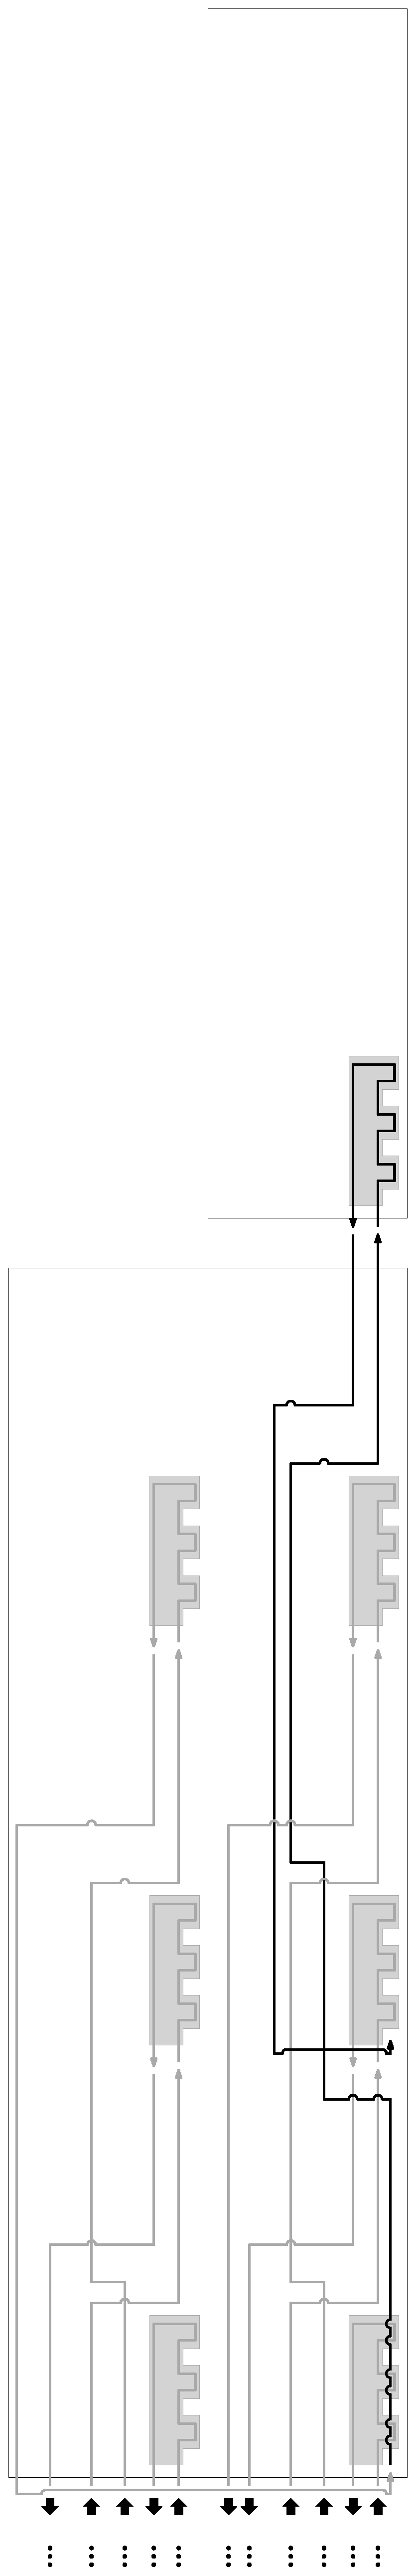
\includegraphics[width=0.6in]{counter_read_digit1_return_read_digit2_general_case3_middle_level}
        \caption{\label{fig:counter_read_digit1_return_read_digit2_general_case3_middle_level} Digit 1 in row $i$ is read, and row $i + 1$ is started. After this digit is
        written, the counter returns to row $i$, and is read to read digit 2.}
    \end{subfigure}%
    ~
    \begin{subfigure}[t]{0.2\textwidth}
        \centering
        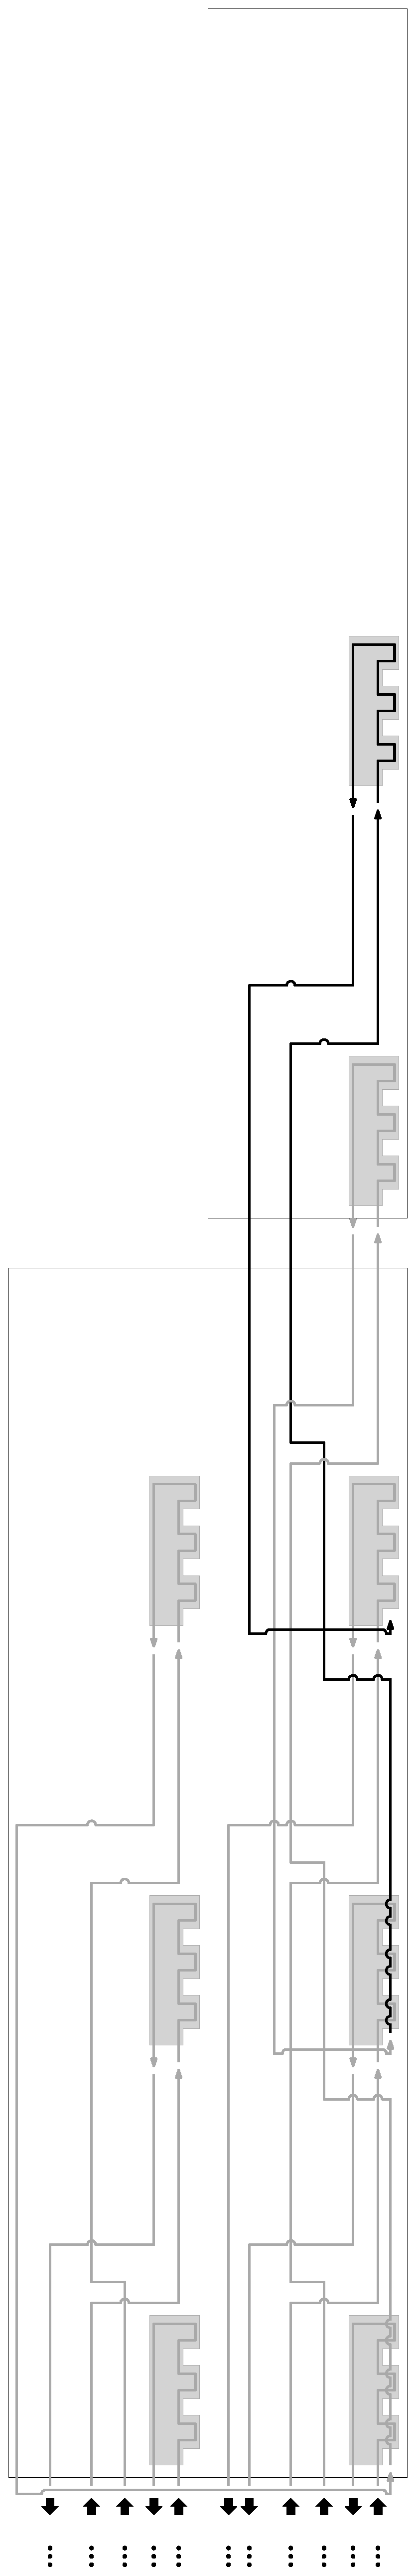
\includegraphics[width=0.6in]{counter_read_digit2_return_read_digit3_general_case3_middle_level}
        \caption{\label{fig:counter_read_digit2_return_read_digit3_general_case3_middle_level} Reading digit 2, writing digit 2 in the next row, and returning to read digit 3 of the current row. }
    \end{subfigure}%
    ~
    \begin{subfigure}[t]{0.2\textwidth}
        \centering
        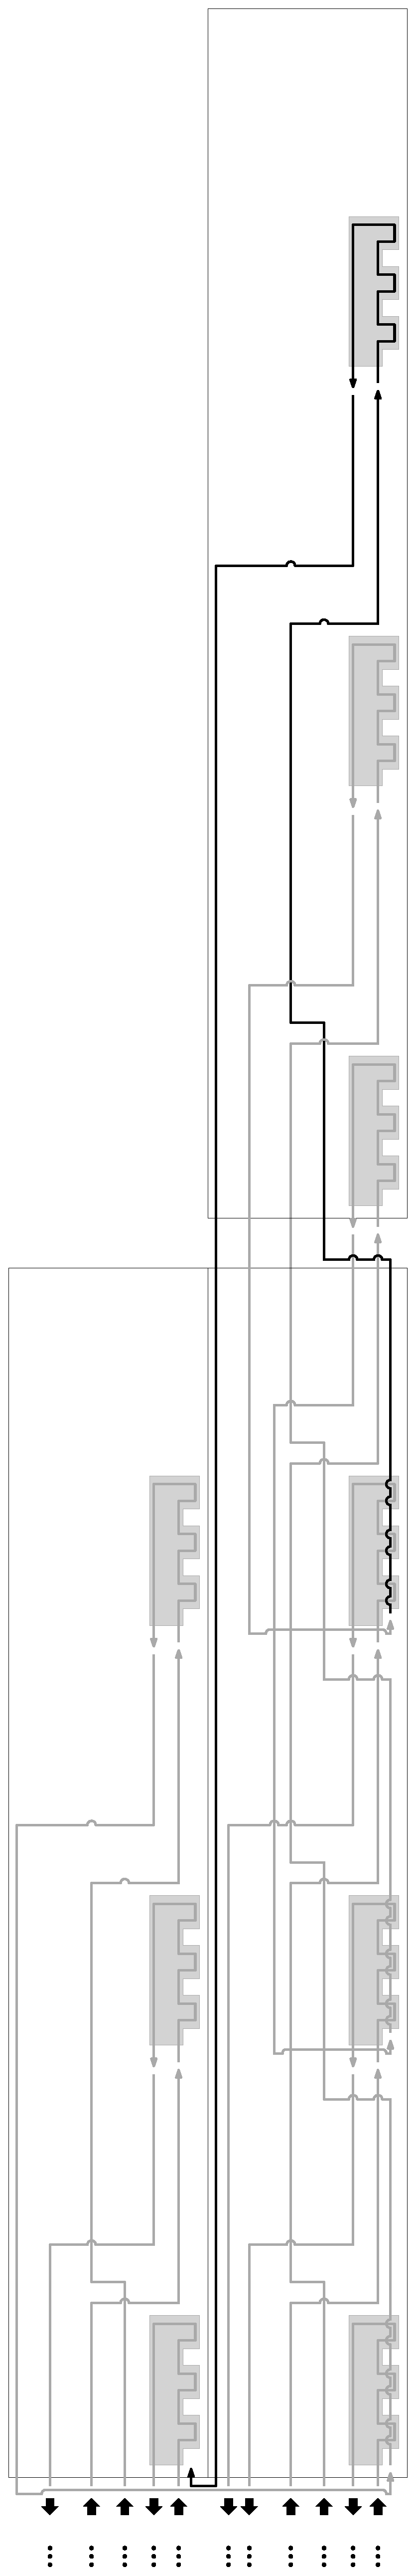
\includegraphics[width=0.6in]{counter_read_digit3_return_read_digit1_general_case3_middle_level}
        \caption{\label{fig:counter_read_digit3_return_read_digit1_general_case3_middle_level} Reading digit 3, writing digit 3 in the next row, and returning to read digit 4 of the current row.}
    \end{subfigure}%

    \caption{\label{fig:counter_read_digit_return_read_digit_general_case3}
    These illustrate how the counter reads and writes a digit region, in a general sense.
    The counter starts in the rightmost digit region, and reads the bottomost digit within
    that region. After reading digit 1, the corresponding digit region will be started in
    row $i + 1$. The counter writes the first digit, and then returns to digit 2 in row $i$.
    Once all the digits in the current digit region are read and written into row $i + 1$,
    the counter can then move to the next digit region in row $i$, begin reading row $i + 1$
    , or halt, depending on what signals are encoded in the geometry of the current row.}

\end{figure}



\section{Tile set}
\label{gadgets}


\newcommand{\warpunit}{{\tt Warp\_Unit}}

\newcommand{\cread}{{\tt Counter\_Read}}
\newcommand{\prewarp}{{\tt Pre\_Warp}}
\newcommand{\firstwarp}{{\tt First\_Warp}}
\newcommand{\warpbridge}{{\tt Warp\_Bridge}}
\newcommand{\secondwarp}{{\tt Second\_Warp}}
\newcommand{\postwarp}{{\tt Post\_Warp}}
\newcommand{\cwrite}{{\tt Counter\_Write}}
\newcommand{\dtop}{{\tt Digit\_Top}}
\newcommand{\returnpath}{{\tt Return\_Path}}
\newcommand{\nextread}{{\tt Next\_Read}}
\newcommand{\crossnextrow}{{\tt Cross\_Next\_Row}}
\newcommand{\roofunit}{{\tt Roof\_Unit}}
\newcommand{\roofscaffolding}{{\tt Roof\_Scaffolding}}
\newcommand{\roofshingle}{{\tt Roof\_Shingle}}
\newcommand{\ops}{\{ {\tt increment}, {\tt copy}, {\tt halt} \}}
\newcommand{\upperbound}{N^{\frac{1}{\floor*{\frac{k}{2}}}}}
\newcommand{\bigom}{O\left(m \right) = O\left( \upperbound \right)}
\newcommand{\inc}{ op}

% todo: fix wording
When describing a special case, i.e. ``digit $x$ -- case $y$'', whatever follows
will only apply to the MSR (due to each case only affecting the MSR.)

\subsection{Gadgets}
\subsubsection{Line Gadgets}
\begin{figure}[H]
    \centering
    \begin{subfigure}[t]{0.15\textwidth}
        \centering
        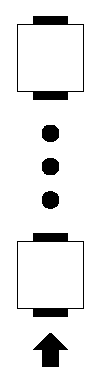
\includegraphics[width=0.15\textwidth]{north_line}
        \caption{\label{fig:north_line} {\tt North\_Line}}
    \end{subfigure}%
    ~
    \begin{subfigure}[t]{0.15\textwidth}
        \centering
        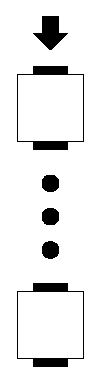
\includegraphics[width=0.15\textwidth]{south_line}
        \caption{\label{fig:south_line} {\tt South\_Line} }
    \end{subfigure}%
    ~
    \caption{\label{fig:line_gadgets} {\tt Line} gadgets}
\end{figure}

We will use the notation {\tt NorthN\_Line} and {\tt SouthN\_Line} where {\tt N} corresponds to the length of a specific line gadget.

\subsubsection{ \cread }

\begin{itemize}
% 0 to l - 1 means L
% 0 to l - 2 means L - 1
% 2MSB:  in: L-2,  out=L-1
% MSB;    in: L-1 , out=L
\item For each $i = 1,2,3$,
               $j = 0,\ldots,l-2$,
               $u \in \{0, 1\}^j$, and
               $\inc \in \{{\tt increment}, {\tt copy} \}$:
    \begin{itemize}
        \item if $j = 0$:
        create
        $\begin{aligned}[t]
            \cread(& \left\langle {\tt CounterRead}, i, \lambda, \inc \right\rangle, \\
                   & \left\langle {\tt CounterRead}, i, 0,      \inc \right\rangle, \\
                   & \left\langle {\tt CounterRead}, i, 1,      \inc \right\rangle \;)
        \end{aligned}$\\ from the general gadget in Figure~\ref{fig:counter_read}.

        \item else:
        create $\begin{aligned}[t]
        \cread(& \left\langle {\tt CounterRead}, i, u,  \inc \right\rangle, \\
               & \left\langle {\tt CounterRead}, i, 0u, \inc \right\rangle, \\
               & \left\langle {\tt CounterRead}, i, 1u, \inc \right\rangle \;)
        \end{aligned}$\\ from the general gadget in Figure~\ref{fig:counter_read}.
    \end{itemize}

\end{itemize}

\begin{itemize}

    \item For each $i = 1,2,3$ and each $u \in \{0, 1\}^{l-1}$:

    \begin{itemize}
        \item Create $\begin{aligned}[t]
            \cread(& \left\langle {\tt CounterRead}, i,  u, {\tt copy} \right\rangle,
                     \left\langle {\tt PreWarp},     i, 0u, {\tt copy} \right\rangle,
                     \left\langle {\tt PreWarp},     i, 1u, {\tt copy} \right\rangle \;)
        \end{aligned}$\\from the general gadget in Figure~\ref{fig:counter_read}.
    \end{itemize}


Since the counter must only increment the current value if the result will be less than $m$,
the \\{\cread} gadgets that have both an {\tt increment} signal and input size of $l - 2$ must
first right shift the bits 2 spots, and then for each possible value after reading one more bit,
check whether that value is less than $m - 1$. % counting in base-M implies that each digit must be less than M %.
%
Basically, if the next bit read is a 0, we check if the current value + 1 is less than $m$.
%
%
%
% If the counter is counting in base 8, (m is 8), then each digit has 3 (value) + 2 (indicator) bits.
% The max digit value is "111"
% Here we'd be on the last/most significant bit, so we've read "0100", and now let's pretend the next
% bit is a "1", so the output would be "10100" IF this was a copy row.
%
% But we're incrementing, so focusing only on the digit value of "101"...
%
% Since the next bit is in the log(M) - 1's index, this means we must add 2^ log(M) - 1 to
% "01" (the current value). We call this the final value of the digit.
%
% So adding 2^log2(M) - 1 to the final value, we get "101". Then, once we know the final value,
% we check to see if the final value + 1 is less than M. If it is, the digit can be incremented
% and we change the increment signal to a copy signal and pass along the final value + 1 as the next digit
% to write, otherwise we output all zeroes and keep the increment signal.
%
If the next bit read is a 1, we check if current value + $2^{\log (m) - 1}$ + 1 is less than $m$.
%
For both cases, if the counter can increment the current value, then
the {\cread} gadgets output the incremented value to the {\prewarp} gadgets and output a {\tt copy}
signal. Otherwise, if the counter is unable to increment the value, it outputs signal in which the bits
of the digit is all zeroes and it will propagate the {\tt increment} signal to the next digit.

    \begin{algorithm}
        \caption{Incrementing and halting}\label{asda}
        \begin{algorithmic}[1]
            \Function{ReadMSB}{}
                \If{$u$ ends with ``11"}
                    \State $out0 \gets \left\langle {\tt halt} \right\rangle$.
                    \State $out1 \gets \left\langle {\tt halt} \right\rangle$.
                \Else
                    \State $guess0 \gets 0u >> 2$.
                    \State $guess1 \gets 1u >> 2$.
                    \If{$convertToDecimal(guess0) + 1 < m - 1$}
                        \State $out0 \gets \left\langle {\tt PreWarp}, i, convertToBinary(convertToDecimal(guess0) + 1) + u[1] + [0], {\tt copy} \right\rangle$.
                    \Else
                        \State $out0 \gets \left\langle {\tt PreWarp}, i, repeat(``0", m) + u[1] + u[0], {\tt increment} \right\rangle$.
                    \EndIf
                    \If{$convertToDecimal(guess1) + 1 < m - 1$}
                        \State $out1 \gets \left\langle {\tt PreWarp}, i, convertToBinary(convertToDecimal(guess1) + 1) + u[1] + [0], {\tt copy} \right\rangle$.
                    \Else
                        \State $out1 \gets \left\langle {\tt PreWarp}, i, repeat(``0", m) + u[1] + u[0], {\tt increment} \right\rangle$.
                    \EndIf
                \EndIf
            \EndFunction
        \end{algorithmic}
    \end{algorithm}

    \begin{itemize}
        \item
        Create $\begin{aligned}[t]
                   \cread(& \left\langle {\tt CounterRead}, i, u, {\tt increment} \right\rangle, out0, out1 \;)
               \end{aligned}$\\from the general gadget in Figure~\ref{fig:counter_read}.
    \end{itemize}
\end{itemize}

\begin{figure}[H]
    \centering
    \subcaptionbox{
        {\tt Counter\_Read\_0}
        \label{fig:counter_read_0}
    }{\makebox[0.24\textwidth][c]{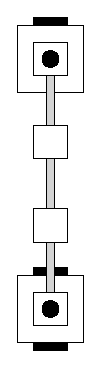
\includegraphics[width=0.33in]{counter_read_0}}}%
    ~
    \subcaptionbox{
        {\tt Counter\_Read\_1}
        \label{fig:counter_read_1}
    }{\makebox[0.24\textwidth][c]{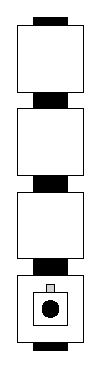
\includegraphics[width=0.33in]{counter_read_1}}}%
    ~
    \subcaptionbox{
        Digit 1 - general\\ overview.
        \label{fig:counter_read_1_op}
    }{\makebox[0.24\textwidth][c]{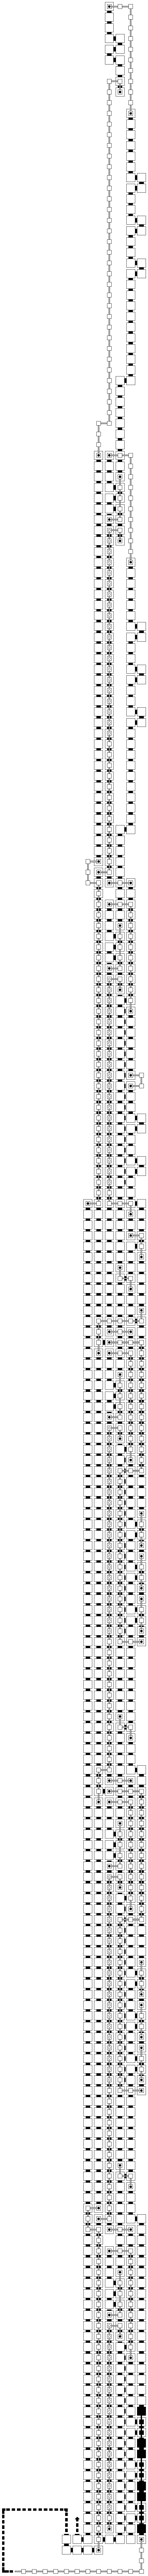
\includegraphics[width=0.45in]{overviews/general/counter_read_1_op}}}%
    ~
    \subcaptionbox{
        Digit 2 - general\\ overview.
        \label{fig:counter_read_2_op}
    }{\makebox[0.24\textwidth][c]{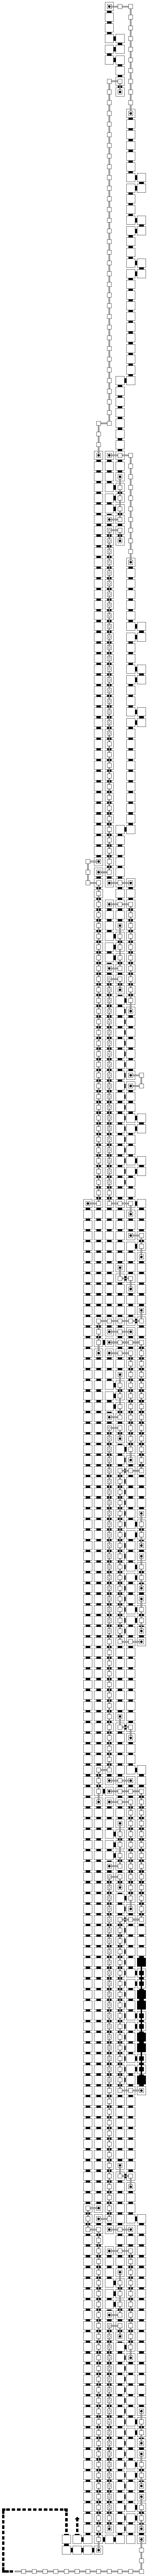
\includegraphics[width=0.45in]{overviews/general/counter_read_2_op}}}%
    ~
\end{figure}
\begin{figure}[H]\ContinuedFloat
    \centering
    \subcaptionbox{
        Digit 3 - general\\ overview.
        \label{fig:counter_read_3_op}
    }{\makebox[0.24\textwidth][c]{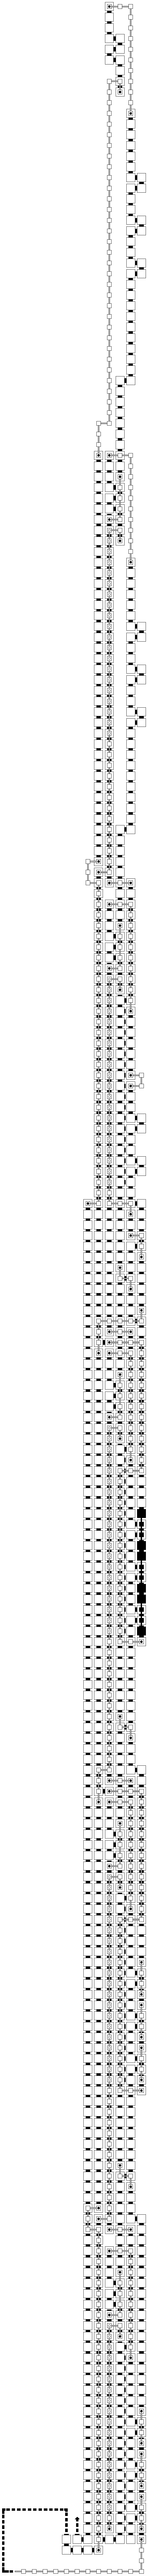
\includegraphics[width=0.45in]{overviews/general/counter_read_3_op}}}%
    ~
    \subcaptionbox{
        Digit 1 - case 1 overview.
        \label{fig:counter_read_1_op_msr_msd}
    }{\makebox[0.24\textwidth][c]{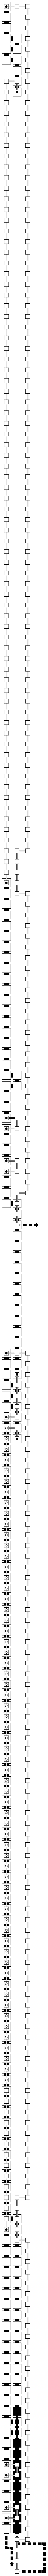
\includegraphics[width=0.45in]{overviews/case1/counter_read_1_op_msr_msd}}}%
    ~
    \subcaptionbox{
        Digit 1 - case 2 overview.
        \label{fig:counter_read_1_op_msr}
    }{\makebox[0.24\textwidth][c]{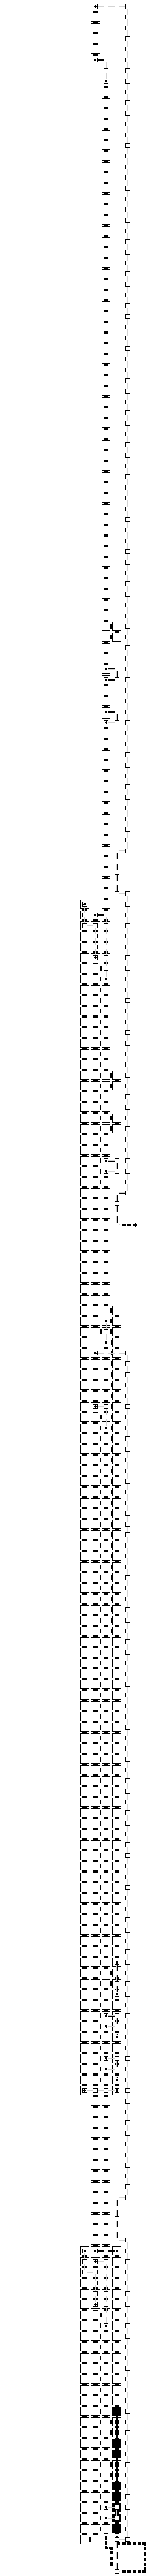
\includegraphics[width=0.45in]{overviews/case2/counter_read_1_op_msr}}}%
    ~
    \subcaptionbox{
        Digit 2 - case 2 overview.
        \label{fig:counter_read_2_op_msr_msd}
    }{\makebox[0.24\textwidth][c]{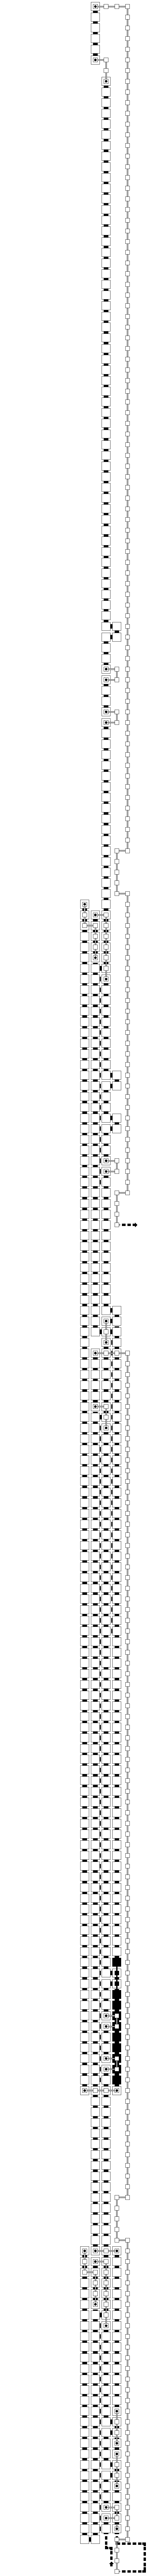
\includegraphics[width=0.45in]{overviews/case2/counter_read_2_op_msr_msd}}}%
    ~
\end{figure}
\begin{figure}[H]\ContinuedFloat
    \centering
    \subcaptionbox{
        Digit 3 - case 3\\ overview.
        \label{fig:counter_read_3_op_msr_msd}
    }{\makebox[0.24\textwidth][c]{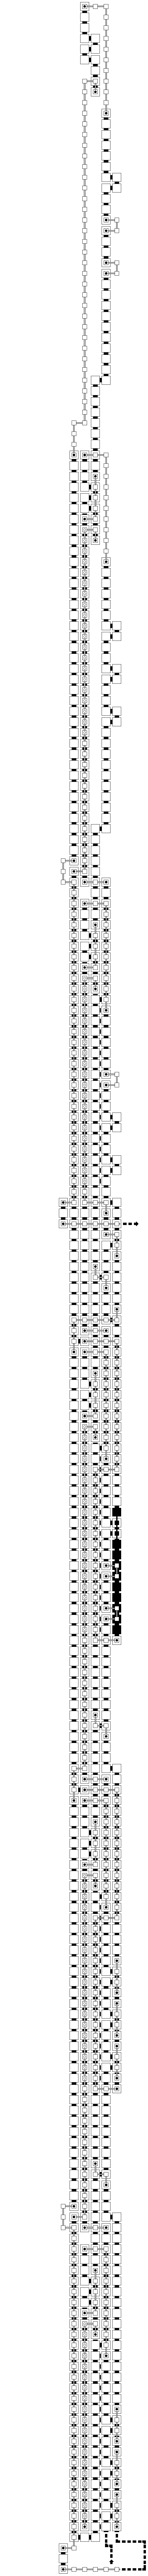
\includegraphics[width=0.45in]{overviews/case3/counter_read_3_op_msr_msd}}}%
    ~
    \caption{\label{fig:counter_read} The {\cread} gadgets.}
\end{figure}
\subsubsection{\warpunit}

We now explain the {\warpunit}. A warp unit generally consists of the following 5 gadgets: \prewarp,
\firstwarp, \warpbridge, \secondwarp, \postwarp. The job of these 5 gadgets is to transport the value
read by the {\cread} all the way to the digit region in the next row, so that the {\cwrite} gadgets
can write the next value in the correct locations. The {\firstwarp} and {\secondwarp} gadgets are single
tile gadgets that have north and south glues with identical labels. This allows the gadgets to continuously
assemble until stopped by earlier parts of the assembly. These single tile gadgets also have one additional glue
that will allow the next piece in the warp unit to assemble, however the assembly will also block this side of the tile
all the way until the gadget can no longer continue assembling in the north direction.

\begin{itemize}

    \item {\prewarp}: These gadgets decode the least significant two bits passed in from
                      the read from the {\cread} gadgets, into a special signal that indicates whether a gadget
                      is currently in the MSR and if it is the MSD. Here is how the signal is decoded: if the least
                      significant bit is 1, add a marker to indicate the current gadgets are in the MSR; if the second least
                      significant bit is also 1, add a marker on the glues to indicate that the gadget is also part
                      of the MSD.

    For each $i = 1,2,3, u \in \{0, 1\}^l$, and each $\inc \in \ops$:
    \begin{itemize}

        \item if $u$ ends with 00:
        create
        $\begin{aligned}[t]
            \prewarp(& \left\langle {\tt PreWarp},   i, u, \inc \right\rangle,
                       \left\langle {\tt FirstWarp}, i, u, \inc \right\rangle \;)
        \end{aligned}$ \\ from the general gadget in Figure~\ref{fig:pre_warp_general}.

        \item if $u$ ends with 01:
        create
        $\begin{aligned}[t]
            \prewarp(& \left\langle {\tt PreWarp},   1, u, \inc            \right\rangle,
                       \left\langle {\tt FirstWarp}, 1, u, \inc, {\tt msr} \right\rangle \;)
        \end{aligned}$ \\ from the general gadget in Figure~\ref{fig:pre_warp_1_op_msr_msd}.


        \item if $u$ ends with 11:
        create
        $\begin{aligned}[t]
            \prewarp(& \left\langle {\tt PreWarp},   i, u, \inc                       \right\rangle,
                       \left\langle {\tt FirstWarp}, i, u, \inc, {\tt msr}, {\tt msd} \right\rangle \;)
        \end{aligned}$ from the general gadget in Figure~\ref{fig:pre_warp_1_op_msr} if $i = 1$ (case 1),
        or Figure~\ref{fig:pre_warp_2_op_msr_msd} if $i = 2$ (case 2), or Figure~\ref{fig:pre_warp_general} if $i = 3$ (case 3).
    \end{itemize}
    \vspace{.5cm}

    \begin{figure}[H]
        \centering
        \subcaptionbox{
            Digits 1, 2, \& 3 - general, Digit 3 - case 3
            \label{fig:pre_warp_general}
        }{\makebox[0.24\textwidth][c]{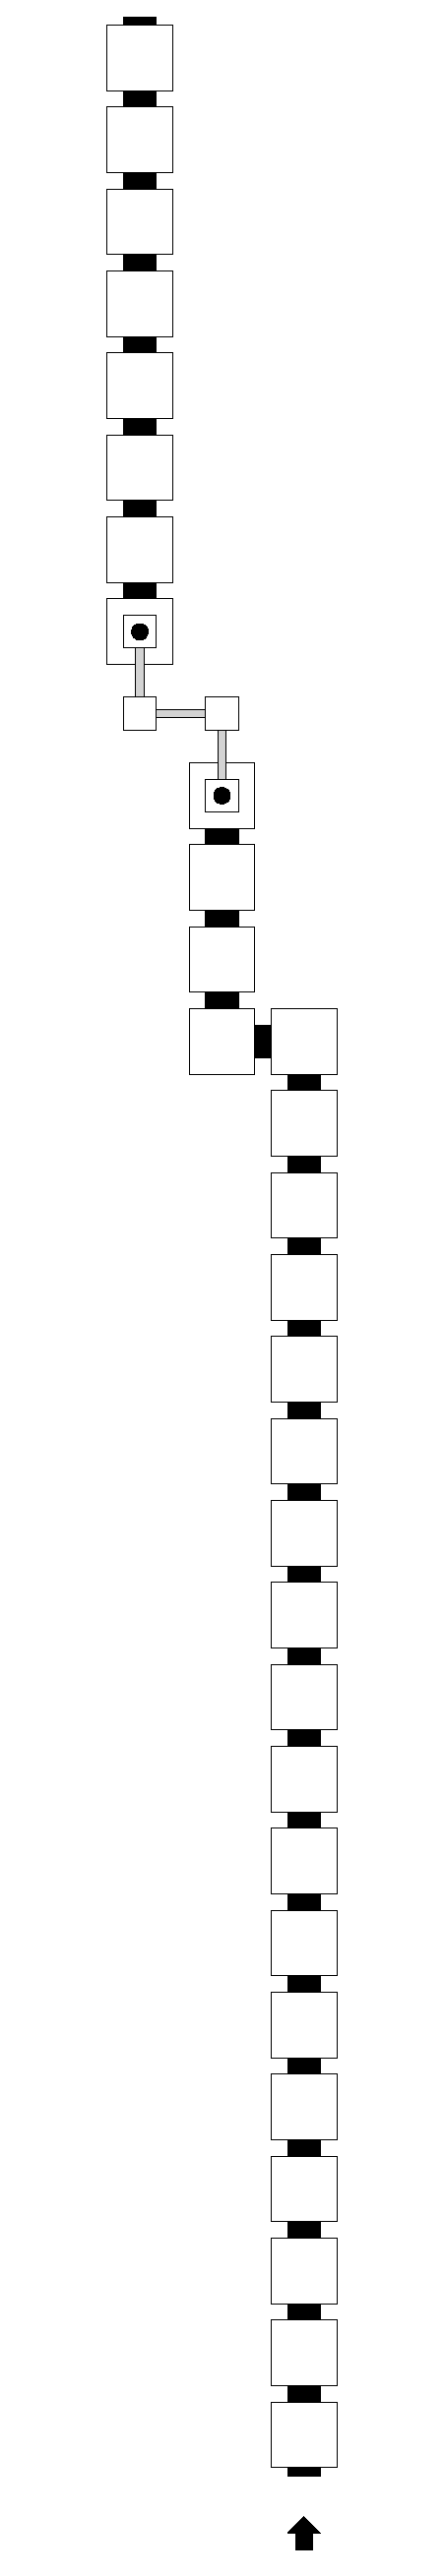
\includegraphics[width=0.45in]{warping_pre_warp_general}}}%
        ~
        \subcaptionbox{
            Digit 1 - general\\overview.
            The black tiles in this figure correspond to the gadget shown in subfigure~\subref{fig:pre_warp_general}.
            \label{fig:pre_warp_1_op_overview}
        }{\makebox[0.24\textwidth][c]{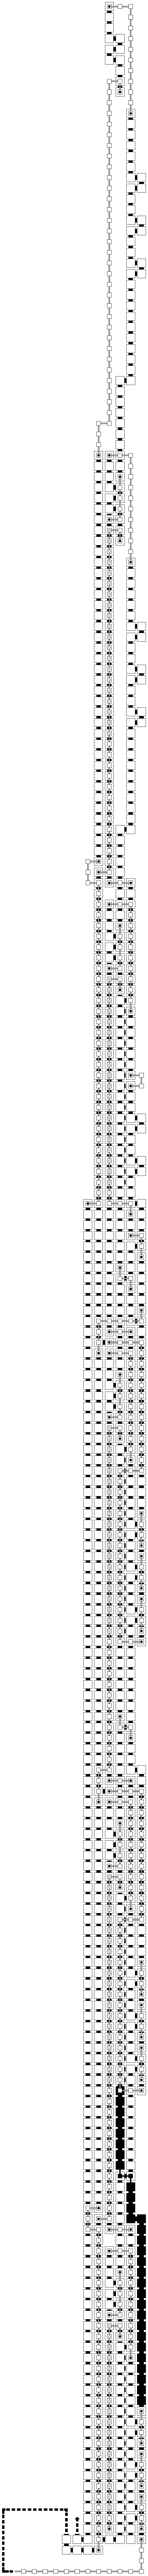
\includegraphics[width=0.45in]{overviews/general/pre_warp_1_op}}}%
        ~
        \subcaptionbox{
            Digit 2 - general\\overview.
            The black tiles in this figure correspond to the gadget shown in subfigure~\subref{fig:pre_warp_general}.
            \label{fig:pre_warp_2_op_overview}
        }{\makebox[0.24\textwidth][c]{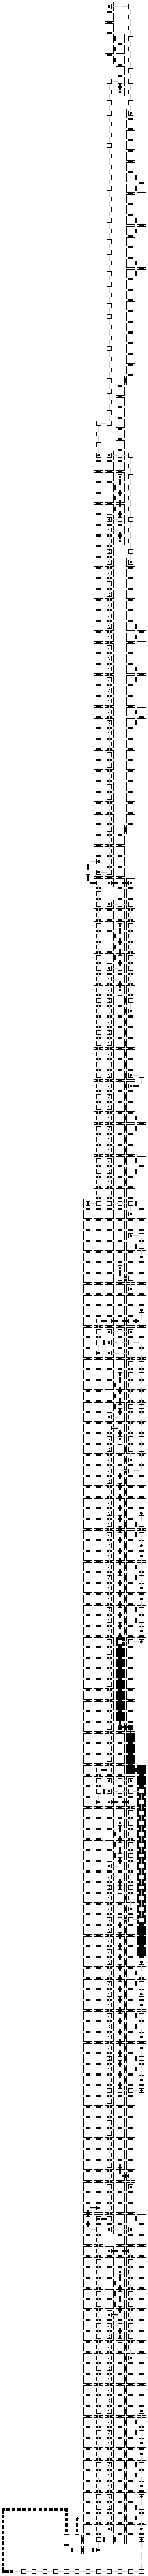
\includegraphics[width=0.45in]{overviews/general/pre_warp_2_op}}}%
        ~
        \subcaptionbox{
            Digit 3 - general\\overview.
            The black tiles in this figure correspond to the gadget shown in subfigure~\subref{fig:pre_warp_general}.
            \label{fig:pre_warp_3_op_overview}
        }{\makebox[0.24\textwidth][c]{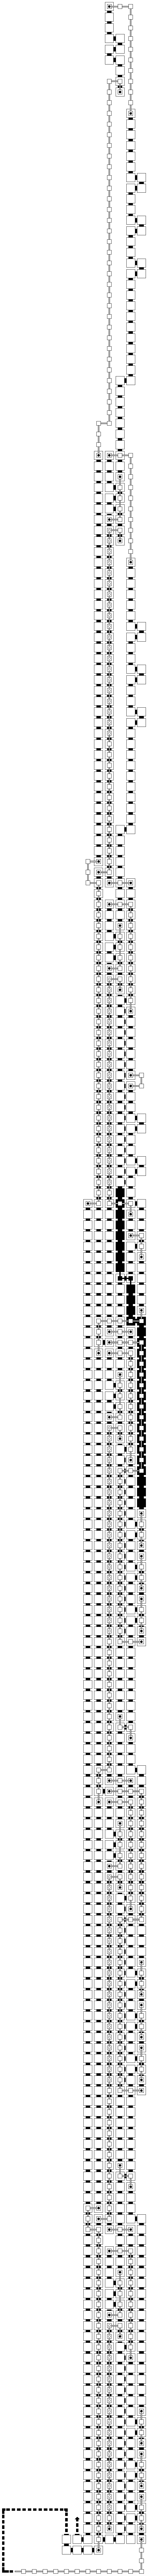
\includegraphics[width=0.45in]{overviews/general/pre_warp_3_op}}}%
        ~
    \end{figure}
    \begin{figure}[H]\ContinuedFloat
        \centering
        \subcaptionbox{
            Digit 1 - case 1.
            \label{fig:pre_warp_1_op_msr_msd}
        }{\makebox[0.24\textwidth][c]{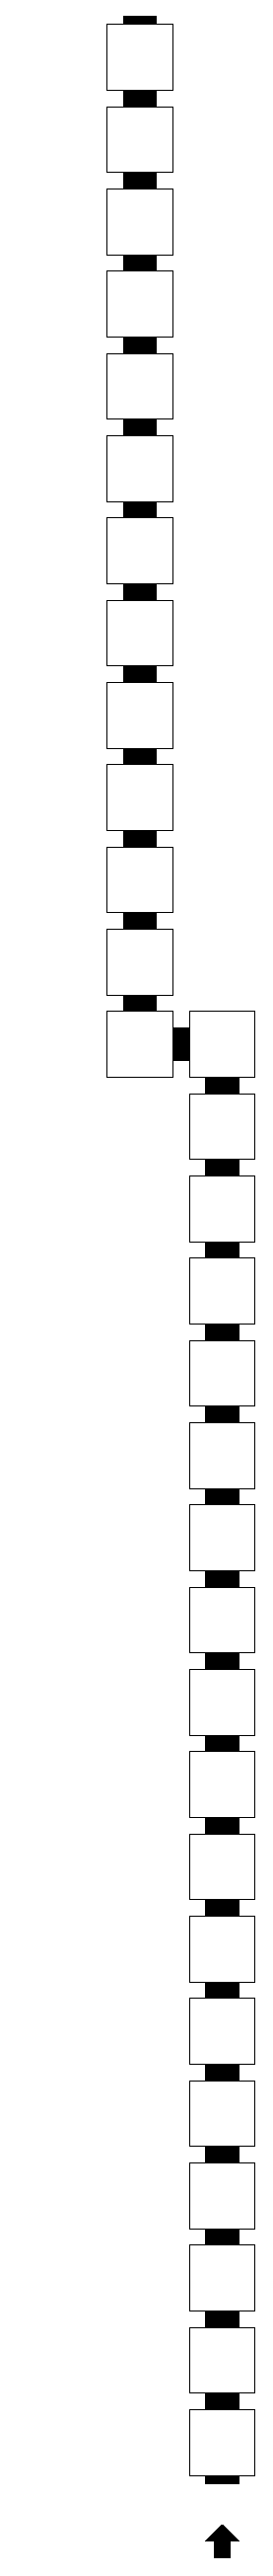
\includegraphics[width=0.45in]{warping_pre_warp_case1_digit1_msr}}}%
        ~
        \subcaptionbox{
            Digit 1 - case 1 overview.
            The black tiles in this figure correspond to the gadget shown in subfigure~\subref{fig:pre_warp_1_op_msr_msd}.
            \label{fig:pre_warp_1_op_msr_msd_overview}
        }{\makebox[0.24\textwidth][c]{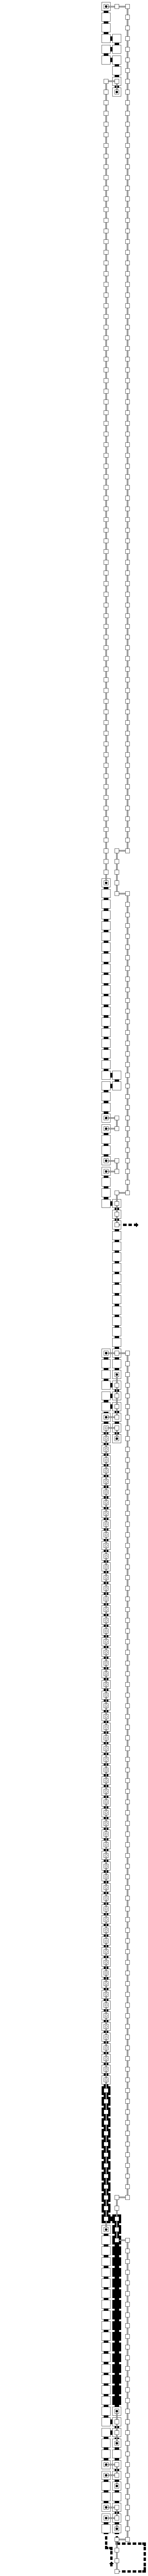
\includegraphics[width=0.45in]{overviews/case1/pre_warp_1_op_msr_msd}}}%
        ~
        \subcaptionbox{
            Digit 1 - case 2.
            \label{fig:pre_warp_1_op_msr}
        }{\makebox[0.24\textwidth][c]{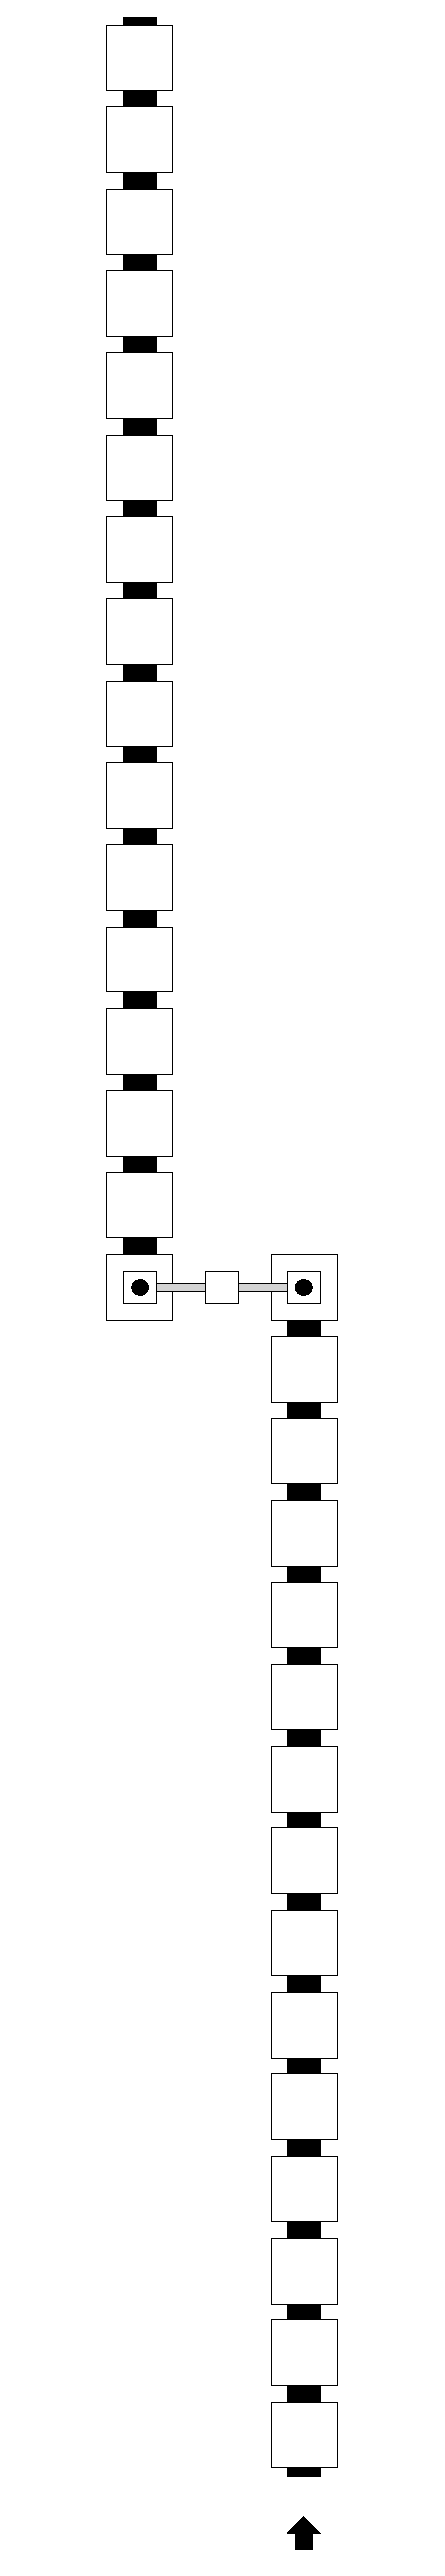
\includegraphics[width=0.45in]{warping_pre_warp_case2_digit1_msr}}}%
        ~
        \subcaptionbox{
            Digit 1 - case 2 overview.
            The black tiles in this figure correspond to the gadget shown in subfigure~\subref{fig:pre_warp_1_op_msr}.
            \label{fig:pre_warp_1_op_msr_overview}
        }{\makebox[0.24\textwidth][c]{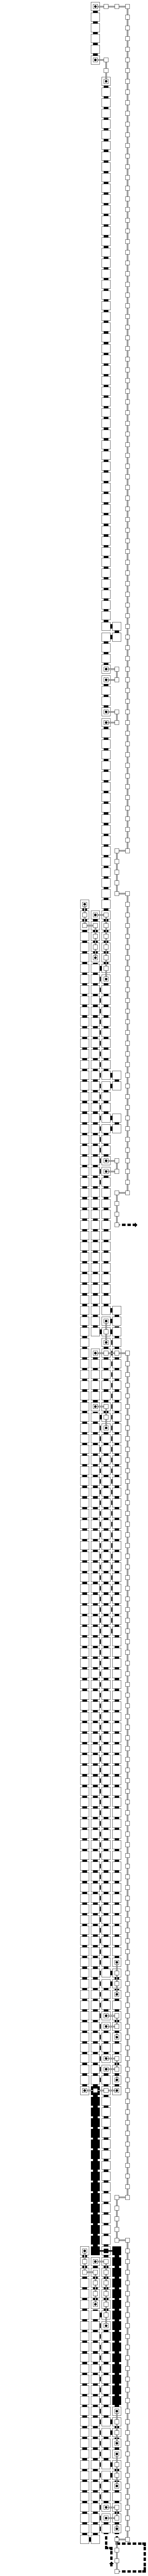
\includegraphics[width=0.45in]{overviews/case2/pre_warp_1_op_msr}}}%
        ~
    \end{figure}

    \begin{figure}[H]\ContinuedFloat
        \centering
        \subcaptionbox{
            Digit 2 - case 2.
            \label{fig:pre_warp_2_op_msr_msd}
        }{\makebox[0.24\textwidth][c]{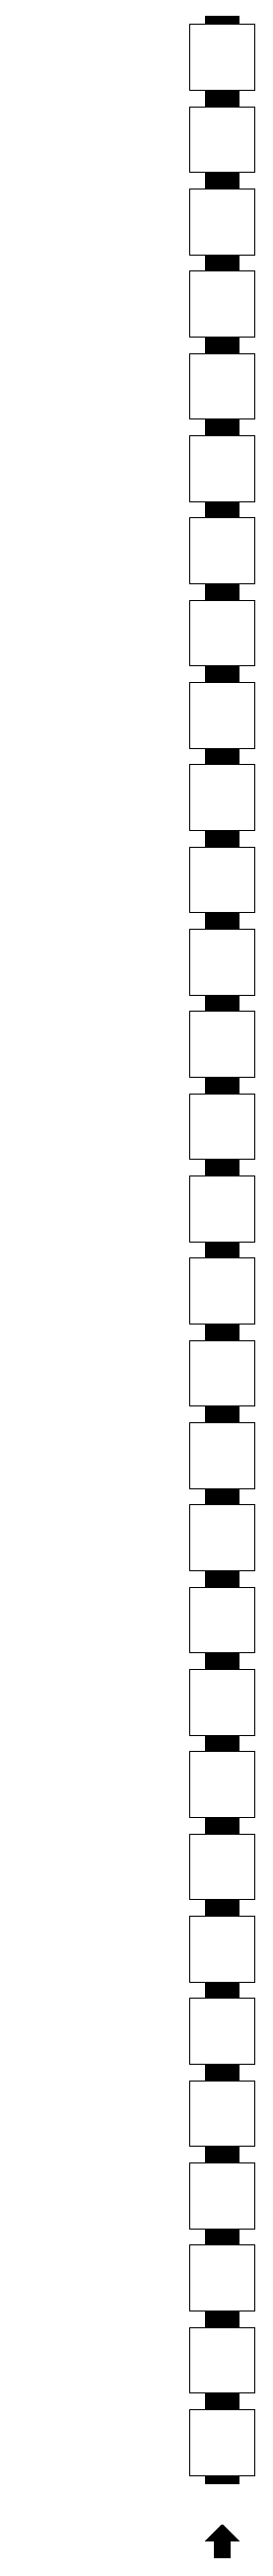
\includegraphics[width=0.45in]{warping_pre_warp_case2_digit2_msr}}}%
        ~
        \subcaptionbox{
            Digit 2 - case 2 overview.
            The black tiles in this figure correspond to the gadget shown in subfigure~\subref{fig:pre_warp_2_op_msr_msd}.
            \label{fig:pre_warp_2_op_msr_msd_overview}
        }{\makebox[0.24\textwidth][c]{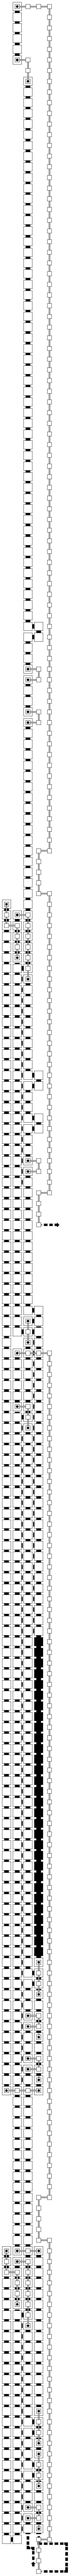
\includegraphics[width=0.45in]{overviews/case2/pre_warp_2_op_msr_msd}}}%
        ~
        \subcaptionbox{
            Digit 3 - case 3 overview.
            The black tiles in this figure correspond to the gadget shown in subfigure~\subref{fig:pre_warp_general}.
            \label{fig:pre_warp_3_op_msr_msd_overview}
        }{\makebox[0.24\textwidth][c]{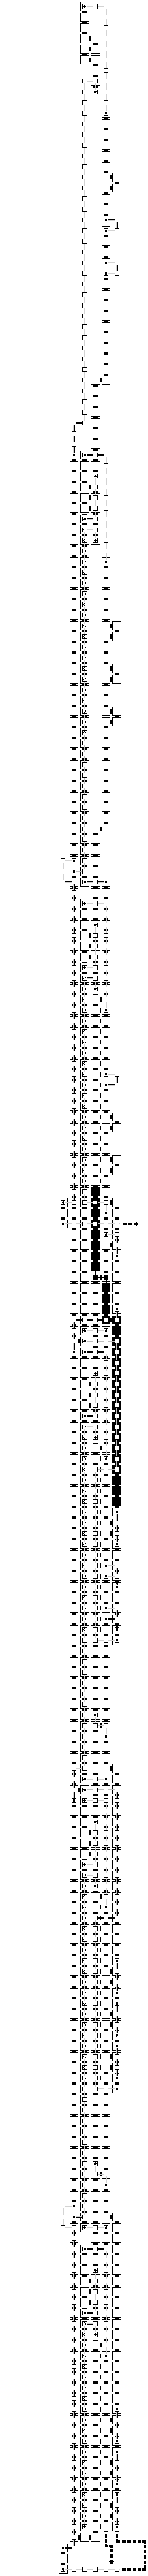
\includegraphics[width=0.45in]{overviews/case3/pre_warp_3_op_msr_msd}}}%
        ~
        \caption{\label{fig:pre_warp_gadgets} The {\prewarp} gadgets. }
    \end{figure}


    \item {\firstwarp}: The idea of the {\firstwarp} gadget is to transport the information read\\
        by the {\cread} gadgets, usually across a distance  $O(\log m)$. We do this using a single tile that
        assembles an infinite line in the north direction, and has one unique glue either in the
        east direction or west direction. This unique glue will at some point later in the assembly, that is
        determined by earlier parts of the assembly, no longer be blocked. When this occurs, it can
        finally attach to the {\warpbridge} gadget (except in a few special cases). This process signifies the ``waking up'' of the
        {\firstwarp} gadgets. When this gadget wakes up, it must also be blocked in the north direction, which
        prevents a truly infinite line from assembling. The geometry required for this process is guarenteed
        to be in place by earlier-assembled {\dtop} gadgets.

        For each $u \in \{0, 1\}^l$, and each $\inc \in \ops$:
        \begin{itemize}

            \item Create
            $\begin{aligned}[t]
                \firstwarp(& \left\langle {\tt FirstWarp},  i, u, \inc \right\rangle,\\  % South
                           & \left\langle {\tt FirstWarp},  i, u, \inc \right\rangle,\\  % North
                           & \left\langle {\tt WarpBridge}, i, u, \inc \right\rangle \;) % East
            \end{aligned}$\\ from the single tile gadget, shown in Figure~\ref{fig:first_warp_1_op_overview}
                             if $i = 1$ or Figure~\ref{fig:first_warp_2_op_overview} if $i = 2$, otherwise from
                             Figure~\ref{fig:first_warp_3_op_overview} if $i = 3$.
            \vspace{.5cm}

            \item Create
            $\begin{aligned}[t]
                \firstwarp(& \left\langle {\tt FirstWarp}, 1, u, \inc, {\tt msr} \right\rangle, \\ % South
                           & \left\langle {\tt FirstWarp}, 1, u, \inc, {\tt msr} \right\rangle, \\ % North
                           & \left\langle {\tt PostWarp},  1, u, \inc, {\tt msr} \right\rangle \;) % East
            \end{aligned}$\\ from the single tile gadget shown in Figure~\ref{fig:first_warp_1_op_msr_overview}.
            \vspace{.5cm}

            \item Create
            $\begin{aligned}[t]
                \firstwarp(& \left\langle {\tt FirstWarp}, 1, u, \inc, {\tt msr}, {\tt msd} \right\rangle, \\ % South
                           & \left\langle {\tt FirstWarp}, 1, u, \inc, {\tt msr}, {\tt msd} \right\rangle, \\ % North
                           & \left\langle {\tt PostWarp},  1, u, \inc, {\tt msr}, {\tt msd} \right\rangle \;) % Up
            \end{aligned}$\\ from the single tile gadget shown in Figure~\ref{fig:first_warp_1_op_msr_msd_overview}.
            \vspace{.5cm}

            \item Create
            $\begin{aligned}[t]
                \firstwarp(& \left\langle {\tt FirstWarp},  2, u, \inc, {\tt msr}, {\tt msd} \right\rangle, \\ % South
                           & \left\langle {\tt FirstWarp},  2, u, \inc, {\tt msr}, {\tt msd} \right\rangle, \\ % North
                           & \left\langle {\tt WarpBridge}, 2, u, \inc, {\tt msr}, {\tt msd} \right\rangle \;) % West
            \end{aligned}$\\ from the single tile gadget shown in Figure~\ref{fig:first_warp_2_op_msr_msd_overview}.
            \vspace{.5cm}

            \item Create
            $\begin{aligned}[t]
                \firstwarp(& \left\langle {\tt FirstWarp},  3, u, \inc, {\tt msr}, {\tt msd} \right\rangle,\\  % South
                           & \left\langle {\tt FirstWarp},  3, u, \inc, {\tt msr}, {\tt msd} \right\rangle,\\  % North
                           & \left\langle {\tt WarpBridge}, 3, u, \inc, {\tt msr}, {\tt msd} \right\rangle \;) % East
            \end{aligned}$\\ from the single tile gadget shown in Figure~\ref{fig:first_warp_3_op_msr_msd_overview}.
            \vspace{.5cm}

        \end{itemize}
        \vspace{.5cm}

    \begin{figure}[H]
        \centering
        \subcaptionbox{
            Digit 1 - general\\ overview.
            \label{fig:first_warp_1_op_overview}
        }{\makebox[0.24\textwidth][c]{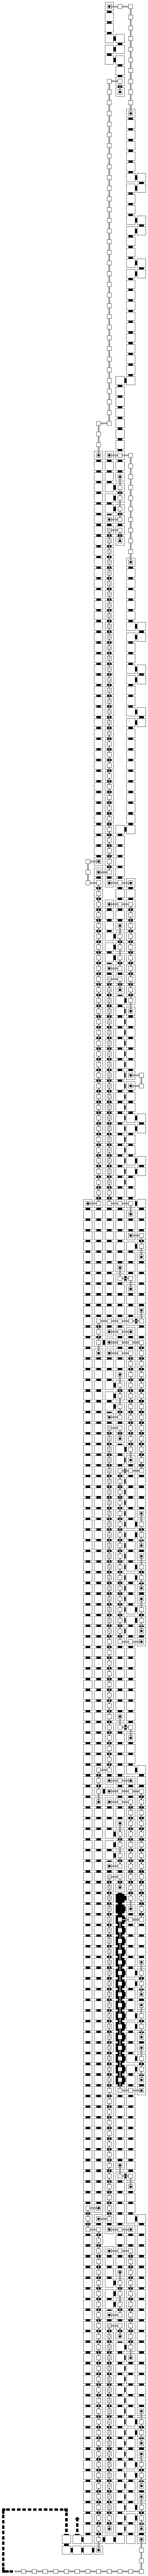
\includegraphics[width=0.45in]{overviews/general/first_warp_1_op}}}%
        ~
        \subcaptionbox{
            Digit 2 - general\\ overview.
            \label{fig:first_warp_2_op_overview}
        }{\makebox[0.24\textwidth][c]{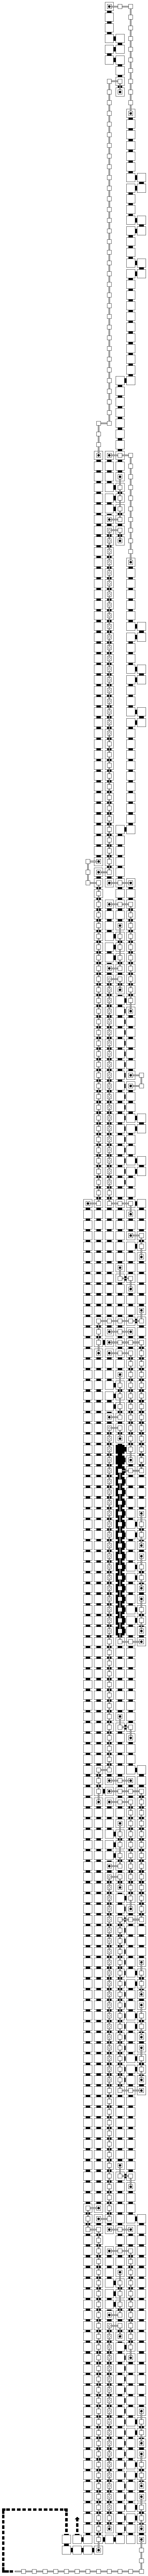
\includegraphics[width=0.45in]{overviews/general/first_warp_2_op}}}%
        ~
        \subcaptionbox{
            Digit 3 - general\\ overview.
            \label{fig:first_warp_3_op_overview}
        }{\makebox[0.24\textwidth][c]{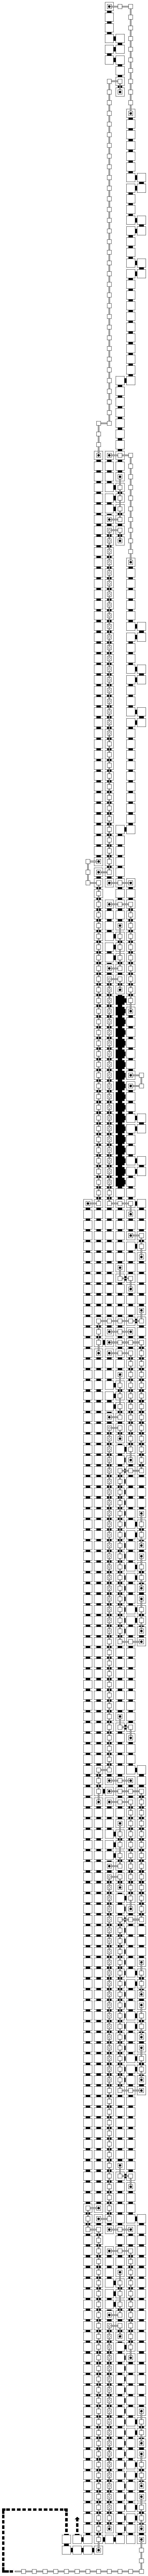
\includegraphics[width=0.45in]{overviews/general/first_warp_3_op}}}%
        ~
        \subcaptionbox{
            Digit 3 - general (seed) overview.
            \label{fig:first_warp_3_seed_op_overview}
        }{\makebox[0.24\textwidth][c]{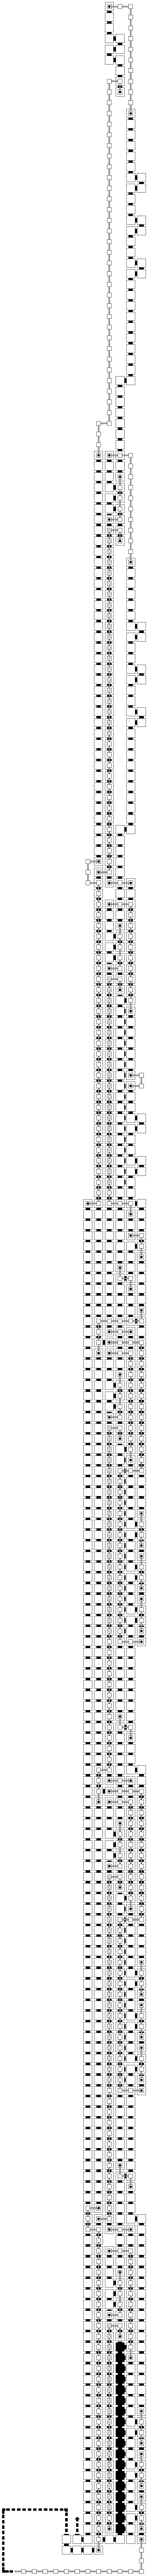
\includegraphics[width=0.45in]{overviews/general/first_warp_3_seed_op}}}%
        ~
    \end{figure}

    \begin{figure}[H]\ContinuedFloat
        \centering
        \subcaptionbox{
            Digit 1 - case 1 overview.
            \label{fig:first_warp_1_op_msr_msd_overview}
        }{\makebox[0.24\textwidth][c]{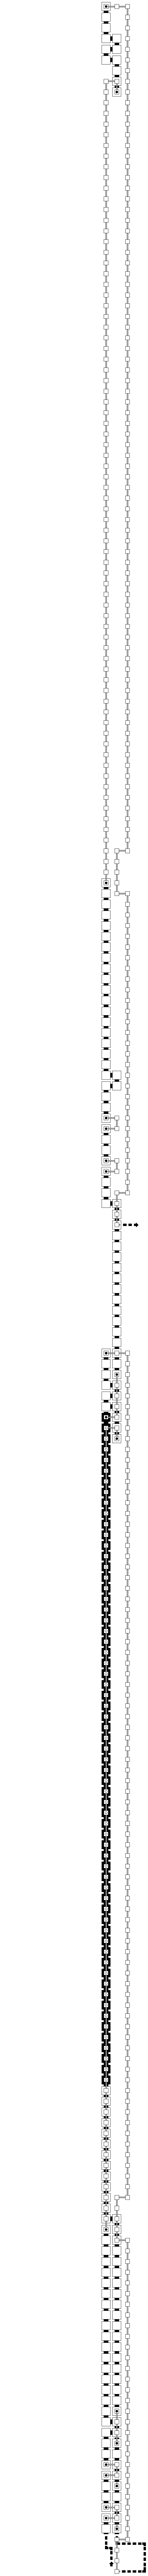
\includegraphics[width=0.45in]{overviews/case1/first_warp_1_op_msr_msd}}}%
        ~
        \subcaptionbox{
            Digit 1 - case 2 overview.
            \label{fig:first_warp_1_op_msr_overview}
        }{\makebox[0.24\textwidth][c]{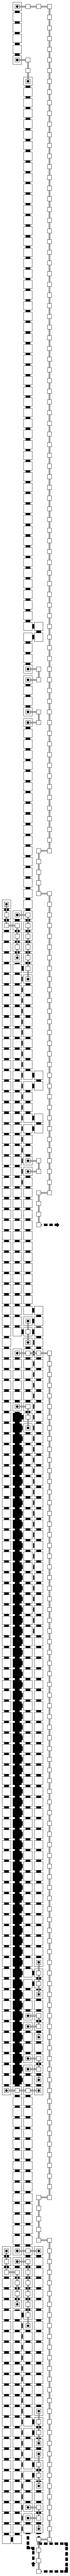
\includegraphics[width=0.45in]{overviews/case2/first_warp_1_op_msr}}}%
        ~
        \subcaptionbox{
            Digit 2 - case 2 overview.
            \label{fig:first_warp_2_op_msr_msd_overview}
        }{\makebox[0.24\textwidth][c]{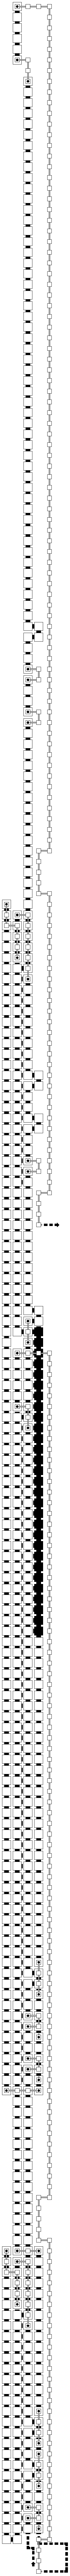
\includegraphics[width=0.45in]{overviews/case2/first_warp_2_op_msr_msd}}}%
        ~
        \subcaptionbox{
            Digit 3 - case 3 overview.
            \label{fig:first_warp_3_op_msr_msd_overview}
        }{\makebox[0.24\textwidth][c]{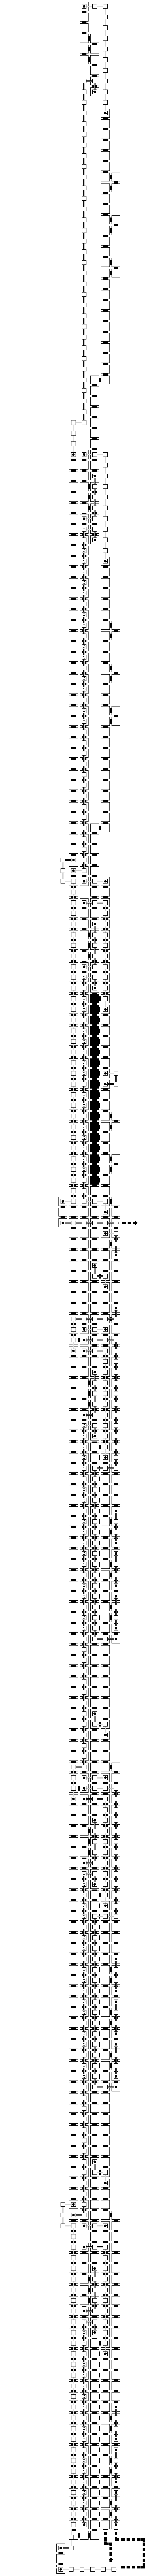
\includegraphics[width=0.45in]{overviews/case3/first_warp_3_op_msr_msd}}}%
        ~
        \caption{\label{fig:first_warp_gadgets_overviews} The {\firstwarp} gadget overviews.}
    \end{figure}


    \item {\warpbridge}: a {\warpbridge} gadget is a gadget which assembles when the {\firstwarp} gadget makes it
         to its final destination. The goal of the {\warpbridge} is to assemble a path from the end of the {\firstwarp}
         gadgets to the start of the {\secondwarp} gadgets. For digit 1 in cases 1 and 2, the {\warpbridge} is omitted
         from the {\warpunit}.

    For each $i = 1,2,3, u \in \{0, 1\}^l$, and each $\inc \in \ops$:
    \begin{itemize}

        \item Create
        $\begin{aligned}[t]
            \warpbridge(& \left\langle {\tt WarpBridge}, i, u, \inc \right\rangle,
                          \left\langle {\tt SecondWarp}, i, u, \inc \right\rangle \;)
        \end{aligned}$ \\ from the general gadget in Figure~\ref{fig:warp_bridge_general}.
        \vspace{.5cm}

        \item Create
        $\begin{aligned}[t]
            \warpbridge(& \left\langle {\tt WarpBridge}, 2, u, \inc, {\tt msr}, {\tt msd} \right\rangle,
                          \left\langle {\tt SecondWarp}, 2, u, \inc, {\tt msr}, {\tt msd} \right\rangle \;)
        \end{aligned}$ \\ from the general gadget in Figure~\ref{fig:warp_bridge_2_op_msr_msd}.
        \vspace{.5cm}

        \item Create
        $\begin{aligned}[t]
            \warpbridge(& \left\langle {\tt WarpBridge}, 3, u, \inc, {\tt msr}, {\tt msd} \right\rangle,
                          \left\langle {\tt SecondWarp}, 3, u, \inc, {\tt msr}, {\tt msd} \right\rangle \;)
        \end{aligned}$ \\ from the general gadget in Figure~\ref{fig:warp_bridge_general}.
        \vspace{.5cm}
    \end{itemize}


    \begin{figure}[H]
        \centering
        \subcaptionbox{
            Digits 1, 2, \& 3 general.
            \label{fig:warp_bridge_general}
        }{\makebox[0.24\textwidth][c]{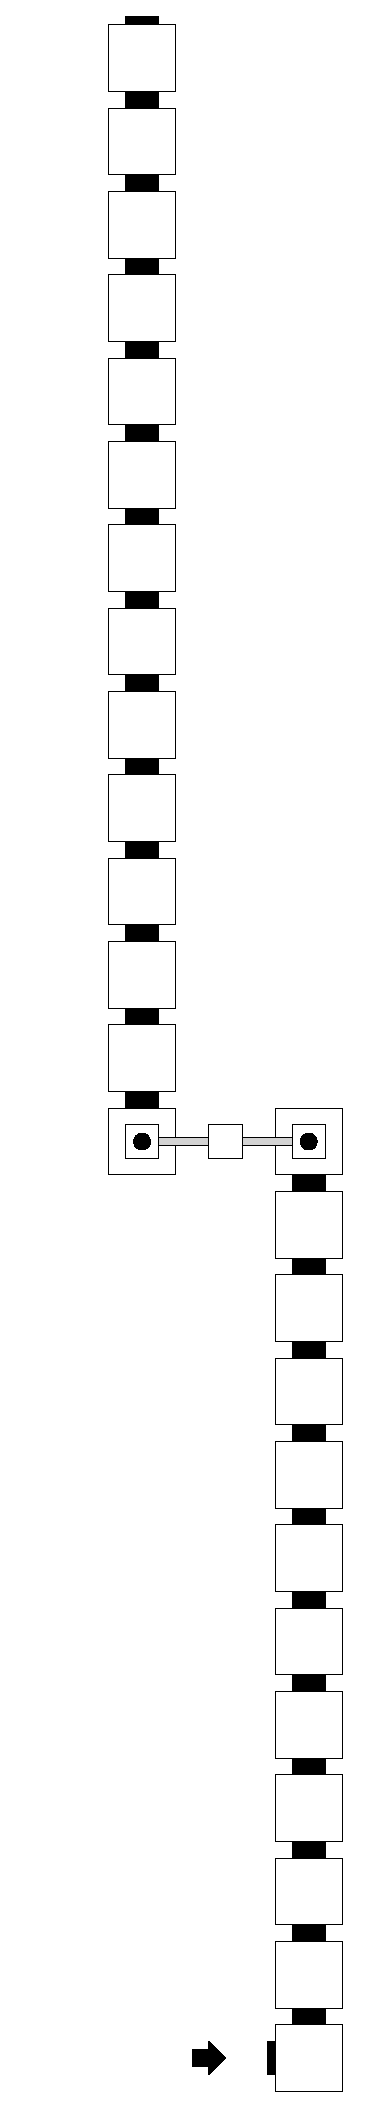
\includegraphics[width=0.45in]{warping_warp_bridge_general}}}%
        ~
        \subcaptionbox{
            Digit 1 - general\\ overview.
            The black tiles in this figure correspond to the gadget shown in subfigure~\subref{fig:warp_bridge_general}.
            \label{fig:warp_bridge_1_op_overview}
        }{\makebox[0.24\textwidth][c]{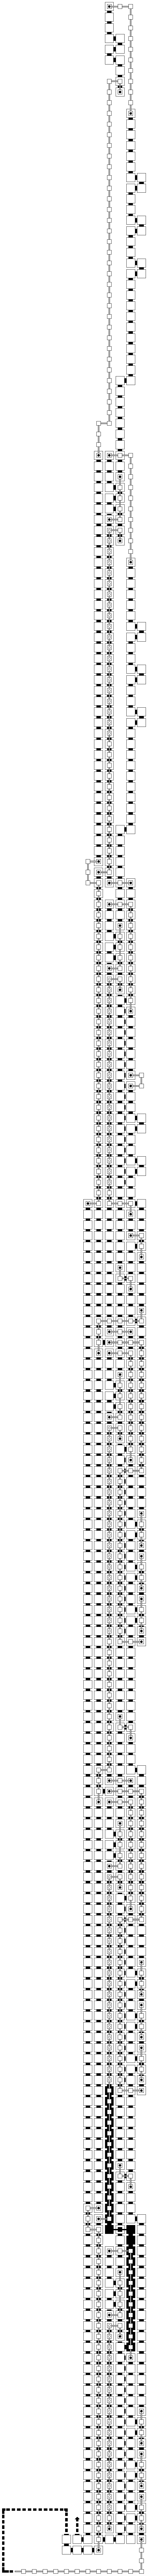
\includegraphics[width=0.45in]{overviews/general/warp_bridge_1_op}}}%
        ~
        \subcaptionbox{
            Digit 2 - general\\ overview.
            The black tiles in this figure correspond to the gadget shown in subfigure~\subref{fig:warp_bridge_general}.
            \label{fig:warp_bridge_2_op_overview}
        }{\makebox[0.24\textwidth][c]{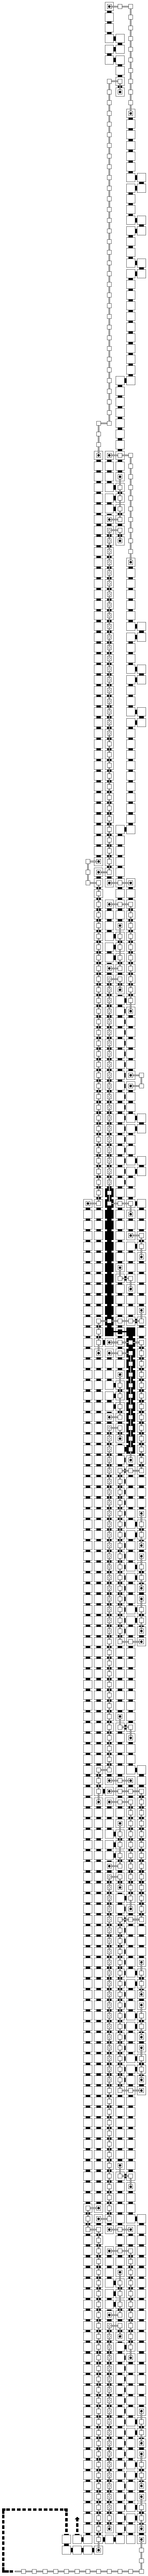
\includegraphics[width=0.45in]{overviews/general/warp_bridge_2_op}}}%
        ~
        \subcaptionbox{
            Digit 2 - general (seed) overview.
            The black tiles in this figure correspond to the gadget shown in subfigure~\subref{fig:warp_bridge_general}.
            \label{fig:warp_bridge_2_seed_op_overview}
        }{\makebox[0.24\textwidth][c]{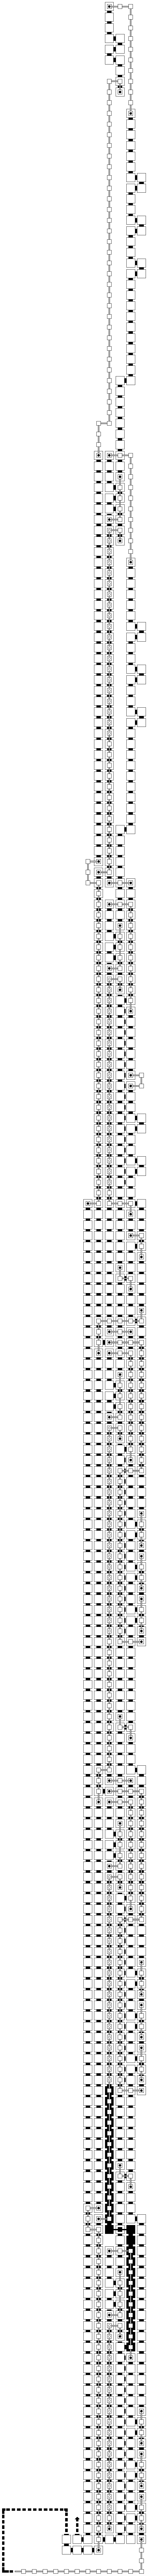
\includegraphics[width=0.45in]{overviews/general/warp_bridge_2_seed_op}}}%
        ~
    \end{figure}
    \begin{figure}[H]\ContinuedFloat
        \centering
        \subcaptionbox{
            Digit 3 - general\\ overview.
            The black tiles in this figure correspond to the gadget shown in subfigure~\subref{fig:warp_bridge_general}.
            \label{fig:warp_bridge_3_op_overview}
        }{\makebox[0.24\textwidth][c]{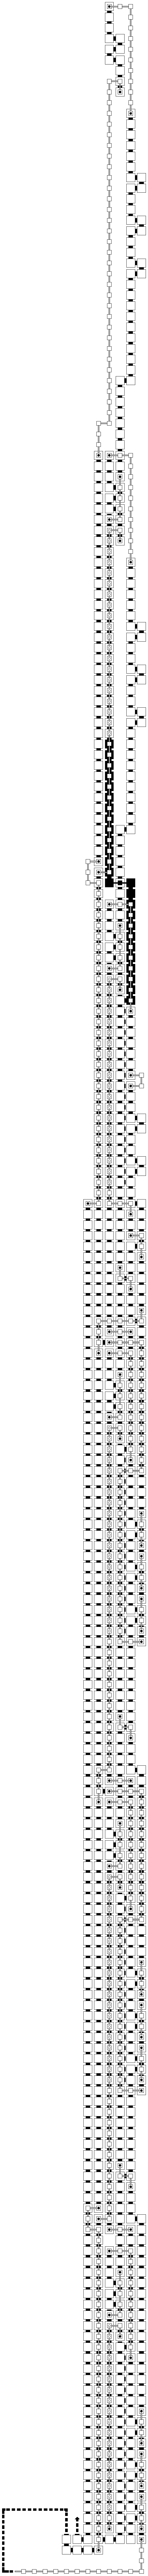
\includegraphics[width=0.45in]{overviews/general/warp_bridge_3_op}}}%
        ~
        \subcaptionbox{
            Digit 3 - general (seed) overview.
            The black tiles in this figure correspond to the gadget shown in subfigure~\subref{fig:warp_bridge_general}.
            \label{fig:warp_bridge_3_seed_op_overview}
        }{\makebox[0.24\textwidth][c]{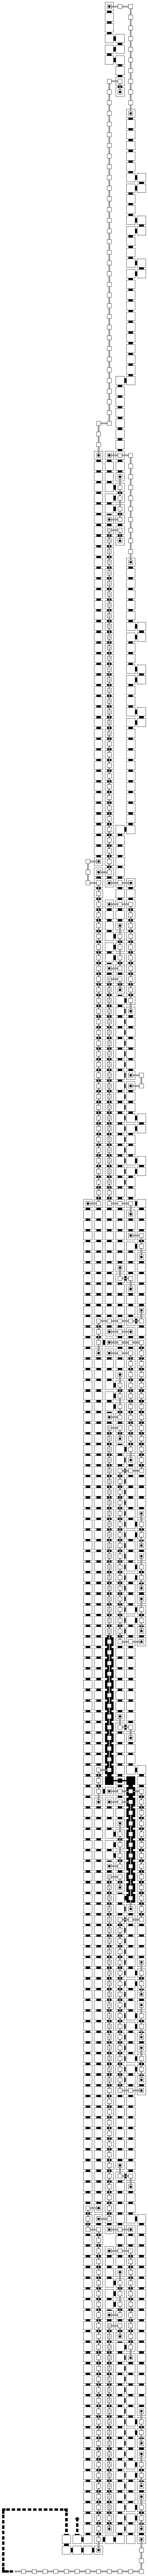
\includegraphics[width=0.45in]{overviews/general/warp_bridge_3_seed_op}}}%
        ~
        \subcaptionbox{
            Digit 2 - case 2.
            \label{fig:warp_bridge_2_op_msr_msd}
        }{\makebox[0.24\textwidth][c]{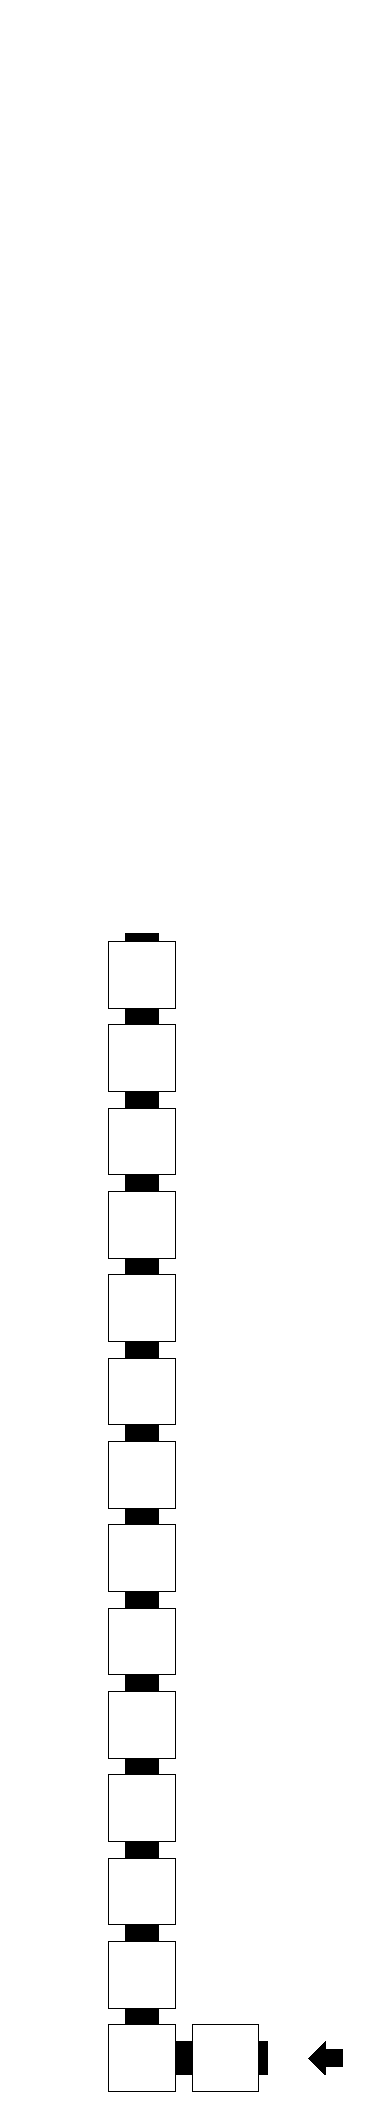
\includegraphics[width=0.45in]{warping_warp_bridge_case2_digit2_msr}}}%
        ~
        \subcaptionbox{
            Digit 2 - case 2 overview.
            The black tiles in this figure correspond to the gadget shown in subfigure~\subref{fig:warp_bridge_2_op_msr_msd}.
            \label{fig:warp_bridge_2_op_msr_msd_overview}
        }{\makebox[0.24\textwidth][c]{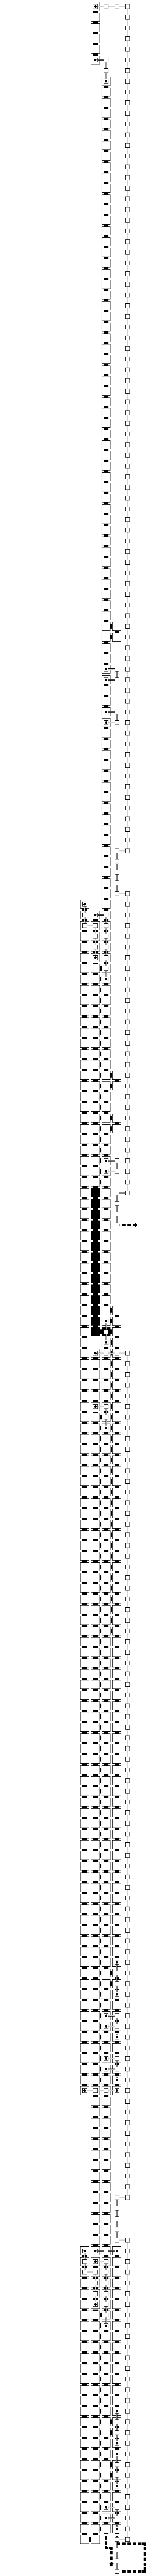
\includegraphics[width=0.45in]{overviews/case2/warp_bridge_2_op_msr_msd}}}%
        ~
    \end{figure}
    \begin{figure}[H]\ContinuedFloat
        \centering
        \subcaptionbox{
            Digit 3 - case 3 overview.
            The black tiles in this figure correspond to the gadget shown in subfigure~\subref{fig:warp_bridge_general}.
            \label{fig:warp_bridge_3_op_msr_msd_overview}
        }{\makebox[0.24\textwidth][c]{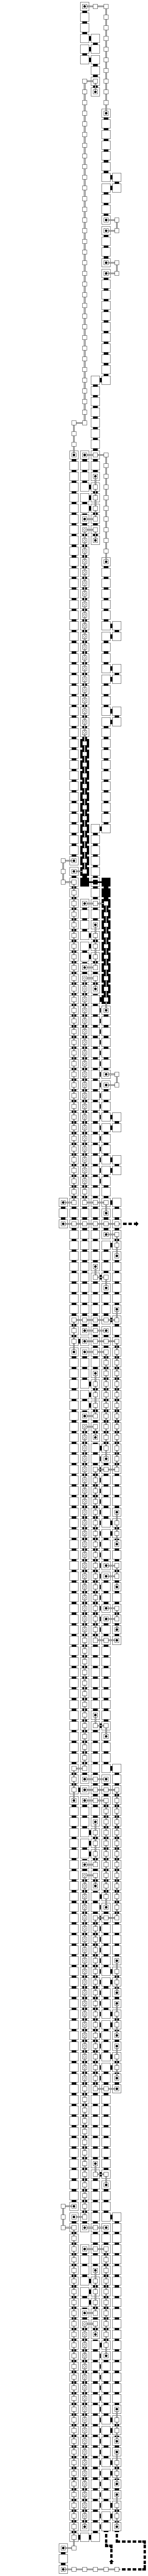
\includegraphics[width=0.45in]{overviews/case3/warp_bridge_3_op_msr_msd}}}%
        ~
        \subcaptionbox{
            Digit 3 - case 3 (seed) overview.
            The black tiles in this figure correspond to the gadget shown in subfigure~\subref{fig:warp_bridge_general}.
            \label{fig:warp_bridge_3_seed_op_msr_msd_overview}
        }{\makebox[0.24\textwidth][c]{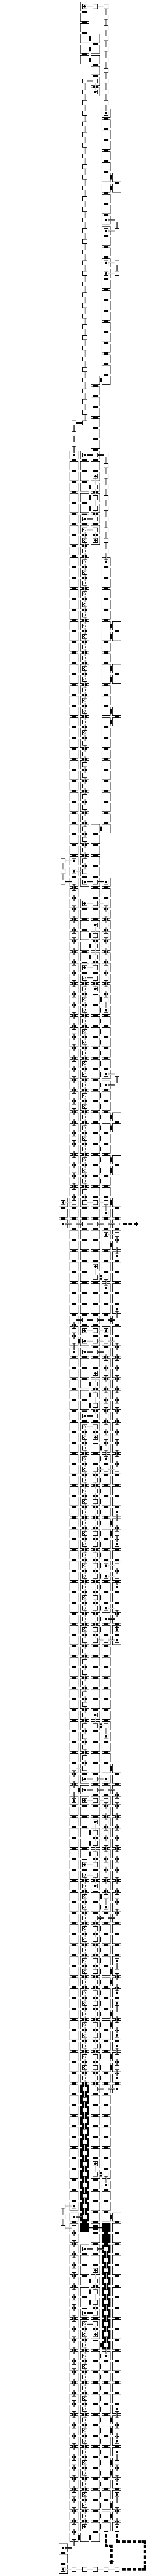
\includegraphics[width=0.45in]{overviews/case3/warp_bridge_3_seed_op_msr_msd}}}%
        ~
        \caption{\label{fig:warp_bridge_gadgets_overviews} The {\warpbridge} gadgets.}
    \end{figure}

    \item {\secondwarp}:
    Similar to the {\firstwarp} gadgets, the idea of the {\secondwarp} gadget is to
    also to transport the information read by the {\cread} gadgets. We do this using a single tile that
    assembles an infinite line in the north direction, and has one unique glue either in the
    east direction or up direction. This unique glue will at some point later in the assembly, that is
    determined by earlier parts of the assembly, no longer be blocked. When this occurs, it can
    finally attach to the {\postwarp} gadget. This process signifies the ``waking up'' of the
    {\secondwarp} gadgets. When this gadget wakes up, it must also be blocked in the north direction, which
    prevent a truly infinite line from assembling. The geometry required for this process is guarenteed
    to be in place by earlier-assembled {\dtop} gadgets.


    For each $i = 1,2,3, u \in \{0, 1\}^l$, and each $\inc \in \ops$:
    \begin{itemize}
        \item Create
        $\begin{aligned}[t]
            \secondwarp(& \left\langle {\tt SecondWarp}, i, u, \inc \right\rangle,     % South
                          \left\langle {\tt SecondWarp}, i, u, \inc \right\rangle,     % North
                          \left\langle {\tt PostWarp},   i, u, \inc \right\rangle \;)  % Up
        \end{aligned}$\\ from the single tile gadget, shown in Figure~\ref{fig:second_warp_1_op_overview}
                         if $i = 1$ or Figure~\ref{fig:second_warp_2_op_overview} if $i = 2$, otherwise from
                         Figure~\ref{fig:second_warp_3_op_overview} if $i = 3$.
        \vspace{0.5cm}

        \item Create
        $\begin{aligned}[t]
            \secondwarp(& \left\langle {\tt SecondWarp}, 2, u, \inc, {\tt msr}, {\tt msd} \right\rangle, \\ % South
                        & \left\langle {\tt SecondWarp}, 2, u, \inc, {\tt msr}, {\tt msd} \right\rangle, \\ % North
                        & \left\langle {\tt PostWarp},   2, u, \inc, {\tt msr}, {\tt msd} \right\rangle \;) % East
        \end{aligned}$\\ from the single tile gadget shown in Figure~\ref{fig:second_warp_2_op_msr_msd_overview}.
        \vspace{0.5cm}

        \item Create
        $\begin{aligned}[t]
            \secondwarp(& \left\langle {\tt SecondWarp}, 3, u, \inc, {\tt msr}, {\tt msd} \right\rangle, \\ % South
                        & \left\langle {\tt SecondWarp}, 3, u, \inc, {\tt msr}, {\tt msd} \right\rangle, \\ % North
                        & \left\langle {\tt PostWarp},   3, u, \inc, {\tt msr}, {\tt msd} \right\rangle \;) % Up
        \end{aligned}$\\ from the single tile gadget shown in Figure~\ref{fig:second_warp_3_op_msr_msd_overview}.
    \end{itemize}

    \begin{figure}[H]
        \centering
        \subcaptionbox{
            Digit 1 - general\\ overview.
            \label{fig:second_warp_1_op_overview}
        }{\makebox[0.24\textwidth][c]{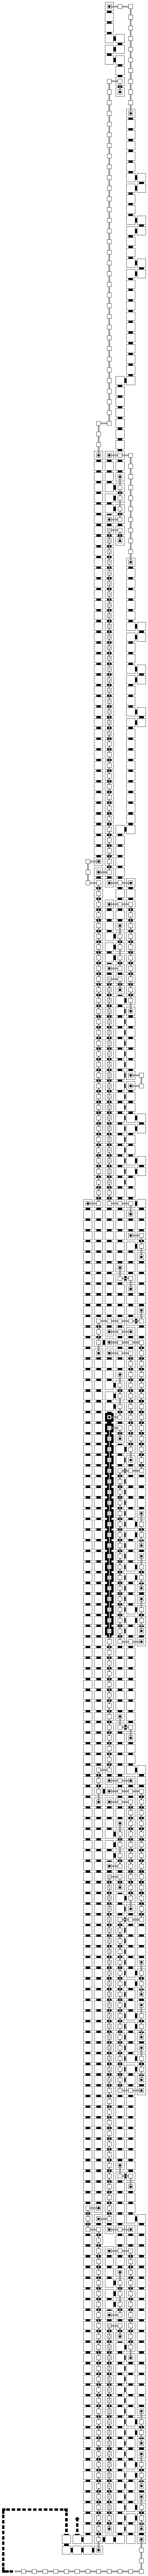
\includegraphics[width=0.45in]{overviews/general/second_warp_1_op}}}%
        ~
        \subcaptionbox{
            Digit 2 - general\\ overview.
            \label{fig:second_warp_2_op_overview}
        }{\makebox[0.24\textwidth][c]{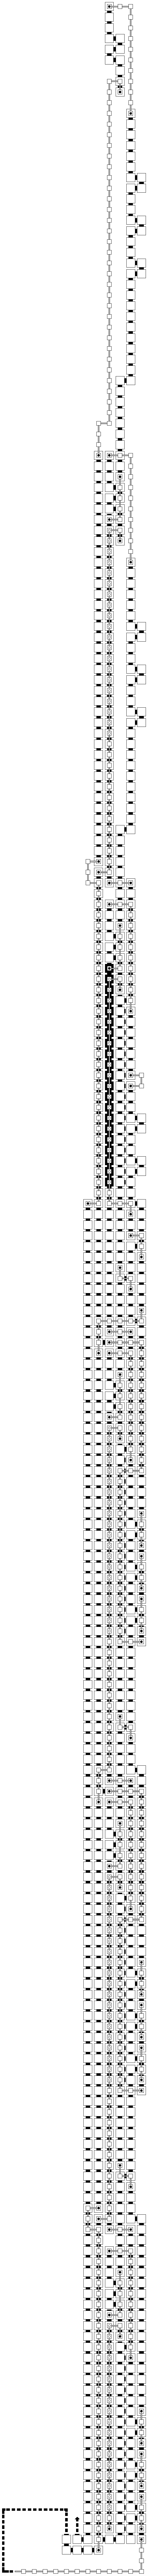
\includegraphics[width=0.45in]{overviews/general/second_warp_2_op}}}%
        ~
        \subcaptionbox{
            Digit 3 - general\\ overview.
            \label{fig:second_warp_3_op_overview}
        }{\makebox[0.24\textwidth][c]{\includegraphics[width=0.45in]{overviews/general/second_warp_3_op}}}%
        ~
        \subcaptionbox{
            Digit 2 - general (seed) overview.
            \label{fig:second_warp_2_seed_op_overview}
        }{\makebox[0.24\textwidth][c]{\includegraphics[width=0.45in]{overviews/general/second_warp_2_seed_op}}}%
        ~
    \end{figure}
    \begin{figure}[H]\ContinuedFloat
        \centering
        \subcaptionbox{
            Digit 3 - general (seed) overview.
            \label{fig:second_warp_3_seed_op_overview}
        }{\makebox[0.24\textwidth][c]{\includegraphics[width=0.45in]{overviews/general/second_warp_3_seed_op}}}%
        ~
        \subcaptionbox{
            Digit 2 - case 2 overview.
            \label{fig:second_warp_2_op_msr_msd_overview}
        }{\makebox[0.24\textwidth][c]{\includegraphics[width=0.45in]{overviews/case2/second_warp_2_op_msr_msd}}}%
        ~
        \subcaptionbox{
            Digit 2 - case 2 (seed) overview.
            \label{fig:second_warp_2_seed_op_msr_msd_overview}
        }{\makebox[0.24\textwidth][c]{\includegraphics[width=0.45in]{overviews/case2/second_warp_2_seed_op_msr_msd}}}%
        ~
        \subcaptionbox{
            Digit 3 - case 3 overview.
            \label{fig:second_warp_3_op_msr_msd_overview}
        }{\makebox[0.24\textwidth][c]{\includegraphics[width=0.45in]{overviews/case3/second_warp_3_op_msr_msd}}}%
        ~
    \end{figure}
    \begin{figure}[H]\ContinuedFloat
        \centering
        \subcaptionbox{
            Digit 3 - case 3 (seed) overview.
            \label{fig:second_warp_3_seed_op_msr_msd_overview}
        }{\makebox[0.24\textwidth][c]{\includegraphics[width=0.45in]{overviews/case3/second_warp_3_seed_op_msr_msd}}}%
        ~
        \caption{\label{fig:second_warp_gadgets_overviews} The {\secondwarp} gadget overviews.}
    \end{figure}


    \item {\postwarp}: The {\postwarp} gadget is final gadget to assemble in the {\warpunit}. The idea of this
    gadget is to assemble from wherever the last warping tiles ``wake up'', forming a path that ends where the
    next digit needs to start being written.

    For each $i = 1,2,3, u \in \{0, 1\}^l$, and each $\inc \in \ops$:
    \begin{itemize}
       \item Create\\
        $\begin{aligned}[t]
            \postwarp(& \left \langle {\tt PostWarp},     i, u, \inc \right\rangle,    % Down
                        \left \langle {\tt CounterWrite}, i, u, \inc \right\rangle \;) % North
        \end{aligned}$ \\
        from the general gadget shown in Figure~\ref{fig:post_warp_1_op} if $i = 1$,
        or Figure~\ref{fig:post_warp_2or3_op} if $ i = 2$ or $i = 3$.
        \vspace{.5cm}


        \item Create
        $\begin{aligned}[t]
            \postwarp(& \left \langle {\tt PostWarp},     1, u, \inc, {\tt msr} \right\rangle,    % West
                        \left \langle {\tt CounterWrite}, 1, u, \inc, {\tt msr} \right\rangle \;) % North
        \end{aligned}$ \\
        from the general gadget in Figure~\ref{fig:post_warp_1_op_msr}.
        \vspace{.5cm}

        \item For each $i=1,2,3$: create\\
        $\begin{aligned}[t]
            \postwarp(& \left \langle {\tt PostWarp},     i, u, \inc, {\tt msr}, {\tt msd} \right\rangle,    % Down if i=1 or i=3, West if i=2
                        \left \langle {\tt CounterWrite}, i, u, \inc, {\tt msr}, {\tt msd} \right\rangle \;) % North
        \end{aligned}$ \\
        from the general gadget shown in Figure~\ref{fig:post_warp_1_op_msr_msd} if $i = 1$, or
        Figure~\ref{fig:post_warp_2_op_msr_msd} if $i = 2$, or Figure~\ref{fig:post_warp_2or3_op} if $i = 3$.
        \vspace{.5cm}

    \end{itemize}

    \begin{figure}[H]
        \centering
        \subcaptionbox{
            Digit 1 - general.
            \label{fig:post_warp_1_op}
        }{\makebox[0.24\textwidth][c]{\includegraphics[width=0.45in]{warping_post_warp_general_digit1}}}%
        ~
        \subcaptionbox{
            Digit 1 - general\\overview.
            The black tiles in this figure correspond to the gadget shown in subfigure~\subref{fig:post_warp_1_op}.
            \label{fig:post_warp_1_op_overview}
        }{\makebox[0.24\textwidth][c]{\includegraphics[width=0.45in]{overviews/general/post_warp_1_op}}}%
        ~
        \subcaptionbox{
            Digit 2 \& 3 - general.
            \label{fig:post_warp_2or3_op}
        }{\makebox[0.24\textwidth][c]{\includegraphics[width=0.45in]{warping_post_warp_general_digit2and3}}}%
        ~
        \subcaptionbox{
            Digit 2 - general\\overview.
            The black tiles in this figure correspond to the gadget shown in subfigure~\subref{fig:post_warp_2or3_op}.
            \label{fig:post_warp_2_op_overview}
        }{\makebox[0.24\textwidth][c]{\includegraphics[width=0.45in]{overviews/general/post_warp_2_op}}}%
        ~
    \end{figure}
    \begin{figure}[H]\ContinuedFloat
        \centering
        \subcaptionbox{
            Digit 2 - general (seed) overview.
            The black tiles in this figure correspond to the gadget shown in subfigure~\subref{fig:post_warp_2or3_op}.
            \label{fig:post_warp_2_seed_op_overview}
        }{\makebox[0.24\textwidth][c]{\includegraphics[width=0.45in]{overviews/general/post_warp_2_seed_op}}}%
        ~
        \subcaptionbox{
            Digit 3 - general\\overview.
            The black tiles in this figure correspond to the gadget shown in subfigure~\subref{fig:post_warp_2or3_op}.
            \label{fig:post_warp_3_op_overview}
        }{\makebox[0.24\textwidth][c]{\includegraphics[width=0.45in]{overviews/general/post_warp_3_op}}}%
        ~
        \subcaptionbox{
            Digit 3 - general (seed) overview.
            The black tiles in this figure correspond to the gadget shown in subfigure~\subref{fig:post_warp_2or3_op}.
            \label{fig:post_warp_3_seed_op_overview}
        }{\makebox[0.24\textwidth][c]{\includegraphics[width=0.45in]{overviews/general/post_warp_3_seed_op}}}%
        ~
        \subcaptionbox{
            Digit 1 - case 1.
            \label{fig:post_warp_1_op_msr_msd}
        }{\makebox[0.24\textwidth][c]{\includegraphics[width=0.45in]{warping_post_warp_case1_digit1_msr}}}%
        ~
    \end{figure}
    \begin{figure}[H]\ContinuedFloat
        \centering
        \subcaptionbox{
            Digit 1 - case 2 overview.
            The black tiles in this figure correspond to the gadget shown in subfigure~\subref{fig:post_warp_1_op_msr_msd}.
            \label{fig:post_warp_1_op_msr_msd_overview}
        }{\makebox[0.24\textwidth][c]{\includegraphics[width=0.45in]{overviews/case1/post_warp_1_op_msr_msd}}}%
        ~
        \subcaptionbox{
            Digit 1 - case 2.
            \label{fig:post_warp_1_op_msr}
        }{\makebox[0.24\textwidth][c]{\includegraphics[width=0.45in]{warping_post_warp_case2_digit1_msr}}}%
        ~
        \subcaptionbox{
            Digit 1 - case 2 overview.
            The black tiles in this figure correspond to the gadget shown in subfigure~\subref{fig:post_warp_1_op_msr}.
            \label{fig:post_warp_1_op_msr_overview}
        }{\makebox[0.24\textwidth][c]{\includegraphics[width=0.45in]{overviews/case2/post_warp_1_op_msr}}}%
        ~
        \subcaptionbox{
            Digit 2 - case 2.
            \label{fig:post_warp_2_op_msr_msd}
        }{\makebox[0.24\textwidth][c]{\includegraphics[width=0.45in]{warping_post_warp_case2_digit2_msr}}}%
        ~
    \end{figure}
    \begin{figure}[H]\ContinuedFloat
        \centering
        \subcaptionbox{
            Digit 2 - case 2\\overview.
            The black tiles in this figure correspond to the gadget shown in subfigure~\subref{fig:post_warp_2_op_msr_msd}.
            \label{fig:post_warp_2_op_msr_msd_overview}
        }{\makebox[0.24\textwidth][c]{\includegraphics[width=0.45in]{overviews/case2/post_warp_2_op_msr_msd}}}%
        ~
        \subcaptionbox{
            Digit 2 - case 2 (seed) overview.
            The black tiles in this figure correspond to the gadget shown in subfigure~\subref{fig:post_warp_2_op_msr_msd}.
            \label{fig:post_warp_2_seed_op_msr_msd_overview}
        }{\makebox[0.24\textwidth][c]{\includegraphics[width=0.45in]{overviews/case2/post_warp_2_seed_op_msr_msd}}}%
        ~
        \subcaptionbox{
            Digit 3 - case 3 overview.
            The black tiles in this figure correspond to the gadget shown in subfigure~\subref{fig:post_warp_2or3_op}.
            \label{fig:post_warp_3_op_msr_msd_overview}
        }{\makebox[0.24\textwidth][c]{\includegraphics[width=0.45in]{overviews/case3/post_warp_3_op_msr_msd}}}%
        ~
        \subcaptionbox{
            Digit 3 - case 3 (seed) overview.
            The black tiles in this figure correspond to the gadget shown in subfigure~\subref{fig:post_warp_2or3_op}.
            \label{fig:post_warp_3_seed_op_msr_msd_overview}
        }{\makebox[0.24\textwidth][c]{\includegraphics[width=0.45in]{overviews/case3/post_warp_3_seed_op_msr_msd}}}%
        ~
        \caption{\label{fig:post_warp_gadgets} The {\postwarp} gadgets.}
    \end{figure}
\end{itemize}

\subsubsection{\cwrite}

\begin{itemize}

    \item For each $i = 1,2,3$,
                   $j = l-1,\ldots,1$,
                   $u \in \{0, 1\}^j$, and each
                   $\inc \in \{{\tt increment}, {\tt copy} \}$:
        \begin{itemize}
        \item Create
        $\begin{aligned}[t]
            \cwrite(& \left\langle {\tt CounterWrite}, i, u0, \inc \right\rangle,
                      \left\langle {\tt CounterWrite}, i, u,  \inc \right\rangle \;)
        \end{aligned}$ \\ from the general gadget in Figure~\ref{fig:counter_write_0}

        \item Create
        $\begin{aligned}[t]
            \cwrite(& \left\langle {\tt CounterWrite}, i,  u1, \inc \right\rangle,
                      \left\langle {\tt CounterWrite}, i,  u,  \inc \right\rangle \;)
        \end{aligned}$ \\ from the general gadget in Figure~\ref{fig:counter_write_1}


        \item Create
        $\begin{aligned}[t]
            \cwrite(& \left\langle {\tt CounterWrite}, 1, u0, \inc, {\tt msr} \right\rangle,
                      \left\langle {\tt CounterWrite}, 1, u,  \inc, {\tt msr} \right\rangle \;)
        \end{aligned}$ \\ from the general gadget in Figure~\ref{fig:counter_write_0}

        \item Create
        $\begin{aligned}[t]
            \cwrite(& \left\langle {\tt CounterWrite}, 1,  u1, \inc, {\tt msr} \right\rangle,
                      \left\langle {\tt CounterWrite}, 1,  u,  \inc, {\tt msr} \right\rangle \;)
        \end{aligned}$ \\ from the general gadget in Figure~\ref{fig:counter_write_1}

        \item Create
        $\begin{aligned}[t]
            \cwrite(& \left\langle {\tt CounterWrite}, i, u0, \inc, {\tt msr}, {\tt msd} \right\rangle,
                      \left\langle {\tt CounterWrite}, i, u,  \inc, {\tt msr}, {\tt msd} \right\rangle \;)
        \end{aligned}$ \\ from the general gadget in Figure~\ref{fig:counter_write_0}

        \item Create
        $\begin{aligned}[t]
            \cwrite(& \left\langle {\tt CounterWrite}, i,  u1, \inc, {\tt msr}, {\tt msd}\right\rangle,
                      \left\langle {\tt CounterWrite}, i,  u,  \inc, {\tt msr}, {\tt msd}\right\rangle \;)
        \end{aligned}$ \\ from the general gadget in Figure~\ref{fig:counter_write_1}
        \end{itemize}

    \item For each $i = 1,2,3$ and each $\inc \in \{{\tt increment}, {\tt copy} \}$:
    \begin{itemize}
        \item Create
        $\begin{aligned}[t]
            \cwrite(& \left\langle {\tt CounterWrite}, i, 0, \inc \right\rangle,
                      \left\langle {\tt DigitTop},     i,    \inc \right\rangle \;)
        \end{aligned}$ \\ from the general gadget in Figure~\ref{fig:counter_write_0}

        \item Create
        $\begin{aligned}[t]
            \cwrite(& \left\langle {\tt CounterWrite}, i, 1, \inc \right\rangle,
                      \left\langle {\tt DigitTop},     i,    \inc \right\rangle \;)
        \end{aligned}$ \\ from the general gadget in Figure~\ref{fig:counter_write_1}

        \item Create
        $\begin{aligned}[t]
            \cwrite(& \left\langle {\tt CounterWrite}, 1, 0, \inc, {\tt msr} \right\rangle,
                      \left\langle {\tt DigitTop},     1,    \inc, {\tt msr} \right\rangle \;)
        \end{aligned}$ \\ from the general gadget in Figure~\ref{fig:counter_write_0}

        \item Create
        $\begin{aligned}[t]
            \cwrite(& \left\langle {\tt CounterWrite}, 1, 1, \inc, {\tt msr} \right\rangle,
                      \left\langle {\tt DigitTop},     1,    \inc, {\tt msr} \right\rangle \;)
        \end{aligned}$ \\ from the general gadget in Figure~\ref{fig:counter_write_1}

        \item Create
        $\begin{aligned}[t]
            \cwrite(& \left\langle {\tt CounterWrite}, i, 0, \inc, {\tt msr}, {\tt msd}\right\rangle,
                      \left\langle {\tt DigitTop},     i,    \inc, {\tt msr}, {\tt msd}\right\rangle \;)
        \end{aligned}$ \\ from the general gadget in Figure~\ref{fig:counter_write_0}

        \item Create
        $\begin{aligned}[t]
            \cwrite(& \left\langle {\tt CounterWrite}, i, 1, \inc, {\tt msr}, {\tt msd}\right\rangle,
                      \left\langle {\tt DigitTop},     i,    \inc, {\tt msr}, {\tt msd}\right\rangle \;)
        \end{aligned}$ \\ from the general gadget in Figure~\ref{fig:counter_write_1}
    \end{itemize}
\end{itemize}

\vspace{.5cm}

\begin{figure}[H]
    \centering
    \subcaptionbox{
        {\tt Counter\_Write\_0}
        \label{fig:counter_write_0}
    }{\makebox[0.24\textwidth][c]{\includegraphics[width=0.45in]{counter_write_0}}}%
    ~
    \subcaptionbox{
        {\tt Counter\_Write\_1}
        \label{fig:counter_write_1}
    }{\makebox[0.24\textwidth][c]{\includegraphics[width=0.45in]{counter_write_1}}}%
    ~
    \subcaptionbox{
        Digit 1 - general\\ overview.
        \label{fig:counter_write_1_op}
    }{\makebox[0.24\textwidth][c]{\includegraphics[width=0.45in]{overviews/general/counter_write_1_op}}}%
    ~
    \subcaptionbox{
        Digit 1 - general (seed) overview.
        \label{fig:counter_write_1_seed_op}
    }{\makebox[0.24\textwidth][c]{\includegraphics[width=0.45in]{overviews/general/counter_write_1_seed_op}}}%
    ~
\end{figure}
\begin{figure}[H]\ContinuedFloat
    \centering
    \subcaptionbox{
        Digit 2 - general\\ overview.
        \label{fig:counter_write_2_op}
    }{\makebox[0.24\textwidth][c]{\includegraphics[width=0.45in]{overviews/general/counter_write_2_op}}}%
    ~
    \subcaptionbox{
        Digit 2 - general (seed) overview.
        \label{fig:counter_write_2_seed_op}
    }{\makebox[0.24\textwidth][c]{\includegraphics[width=0.45in]{overviews/general/counter_write_2_seed_op}}}%
    ~
    \subcaptionbox{
        Digit 3 - general\\ overview.
        \label{fig:counter_write_3_op}
    }{\makebox[0.24\textwidth][c]{\includegraphics[width=0.45in]{overviews/general/counter_write_3_op}}}%
    ~
    \subcaptionbox{
        Digit 3 - general (seed) overview.
        \label{fig:counter_write_3_seed_op}
    }{\makebox[0.24\textwidth][c]{\includegraphics[width=0.45in]{overviews/general/counter_write_3_seed_op}}}%
    ~
\end{figure}
\begin{figure}[H]\ContinuedFloat
    \centering
    \subcaptionbox{
        Digit 1 - case 1.
        \label{fig:counter_write_1_op_msr_msd}
    }{\makebox[0.24\textwidth][c]{\includegraphics[width=0.45in]{overviews/case1/counter_write_1_op_msr_msd}}}%
    ~
    \subcaptionbox{
        Digit 1 - case 1 (seed).
        \label{fig:counter_write_1_op_seed_msr_msd}
    }{\makebox[0.24\textwidth][c]{\includegraphics[width=0.45in]{overviews/case1/counter_write_1_seed_op_msr_msd}}}%
    ~
    \subcaptionbox{
        Digit 1 - case 2.
        \label{fig:counter_write_1_op_msr}
    }{\makebox[0.24\textwidth][c]{\includegraphics[width=0.45in]{overviews/case2/counter_write_1_op_msr}}}%
    ~
    \subcaptionbox{
        Digit 1 - case 2 (seed).
        \label{fig:counter_write_1_op_seed_msr}
    }{\makebox[0.24\textwidth][c]{\includegraphics[width=0.45in]{overviews/case2/counter_write_1_seed_op_msr}}}%
    ~
\end{figure}
\begin{figure}[H]\ContinuedFloat
    \centering
    \subcaptionbox{
        Digit 2 - case 2.
        \label{fig:counter_write_2_op_msr_msd}
    }{\makebox[0.24\textwidth][c]{\includegraphics[width=0.45in]{overviews/case2/counter_write_2_op_msr_msd}}}%
    ~
    \subcaptionbox{
        Digit 2 - case 2 (seed).
        \label{fig:counter_write_2_op_seed_msr_msd}
    }{\makebox[0.24\textwidth][c]{\includegraphics[width=0.45in]{overviews/case2/counter_write_2_seed_op_msr_msd}}}%
    ~
    \subcaptionbox{
        Digit 3 - case 3.
        \label{fig:counter_write_3_op_msr_msd}
    }{\makebox[0.24\textwidth][c]{\includegraphics[width=0.45in]{overviews/case3/counter_write_3_op_msr_msd}}}%
    ~
    \subcaptionbox{
        Digit 3 - case 3 (seed).
        \label{fig:counter_write_3_op_seed_msr_msd}
    }{\makebox[0.24\textwidth][c]{\includegraphics[width=0.45in]{overviews/case3/counter_write_3_seed_op_msr_msd}}}%
    ~
    \caption{\label{fig:counter_write} The {\cwrite} gadgets.}
\end{figure}
\subsubsection{\dtop}

The {\dtop} gadgets have special geometry designed so that {\firstwarp} and
{\secondwarp} tiles are allowed to ``wake up", and complete their warping journey. Each
digit has some type of {\dtop} gadget, however, depending on the digit region
and index of a specific digit, the exact digit top will differ.

% talk about geometry of digit tops enabling first and second warp tiles to "wake up"

\vspace{.5cm}


\begin{figure}[H]
    \centering
    \begin{subfigure}[t]{0.32\textwidth}
        \centering
        \includegraphics[width=0.32\textwidth]{digit_top_general_topper}
        \caption{\label{fig:topper_gen} General topper}
    \end{subfigure}%
    ~
    \begin{subfigure}[t]{0.32\textwidth}
        \centering
        \includegraphics[width=0.32\textwidth]{digit_top_case1_digit1_topper}
        \caption{\label{fig:topper_case1} Case 1 -- topper}
    \end{subfigure}%
    ~
    \begin{subfigure}[t]{0.32\textwidth}
        \centering
        \includegraphics[width=0.32\textwidth]{digit_top_case2_digit2_topper}
        \caption{\label{fig:topper_case2} Case 2 -- topper}
    \end{subfigure}%
    \caption{\label{fig:topper_microgadgets} Topper micro-gadgets }
\end{figure}


For each $\inc \in \{ {\tt increment, copy } \}$
\begin{itemize}

        \item Digit 1 (general): the following statements create the gadget shown in Figure~\ref{fig:digit_top_general}.
        \begin{itemize}
            \item Create
            $\begin{aligned}[t]
                {\tt North\_Line5}(& \left \langle {\tt DigitTop},  1, \inc \right\rangle,
                                     \left \langle {\tt DigitTopA}, 1, \inc \right\rangle \;)
            \end{aligned}$\\from the micro-gadget shown in Figure~\ref{fig:north_line}.

            \item Create
            $\begin{aligned}[t]
                {\tt Topper}(& \left \langle {\tt DigitTopA}, 1, \inc \right\rangle,
                               \left \langle {\tt DigitTopB}, 1, \inc \right\rangle \;)
            \end{aligned}$\\from the micro-gadget shown in Figure~\ref{fig:topper_gen}.

            \item Create
            $\begin{aligned}[t]
                {\tt South\_Line4\textit{l}}(& \left\langle {\tt DigitTopB}, 1, \inc \right\rangle,
                                               \left\langle \returnpath,     1, \inc \right\rangle \;)
            \end{aligned}$\\from the micro-gadget shown in Figure~\ref{fig:south_line}.
        \end{itemize}
        %
        In this step, $2 \cdot \left( 40 + 4l \right) =$
        %
        $80 + 8l =$
        %
        $80 + 8 \cdot \left( \ceil*{\log m} + 2 \right) \leq$
        %
        $80 + 8 \cdot \left( {\log m} + 3 \right) =$
        %
        $104 + 8 \cdot {\log m} = \bigologm$ tiles were created.
        %
        \vspace{0.5cm}


        \item Digit 1 (MSR): the following statements create the gadget shown in Figure~\ref{fig:digit_top_1_op_msr}.
        \begin{itemize}
            \item Create
            $\begin{aligned}[t]
                {\tt Topper}(& \left\langle {\tt DigitTop},  1, \inc, {\tt msr} \right\rangle,
                               \left\langle {\tt DigitTopA}, 1, \inc, {\tt msr} \right\rangle \;)
            \end{aligned}$ \\ from the micro-gadget shown in Figure~\ref{fig:topper_case1}.


            \item Create
            $\begin{aligned}[t]
                {\tt South\_Line4\textit{l}}(& \left\langle {\tt DigitTopA}, 1, \inc, {\tt msr}\right\rangle,
                                               \left\langle \returnpath,     1, \inc, {\tt msr}\right\rangle \;)
            \end{aligned}$ \\ from the micro-gadget shown in Figure~\ref{fig:south_line}.
        \end{itemize}
        %
        In this step, $2 \cdot \left( 43 + 4l \right) =$
        %
        $86 + 8l =$
        %
        $86 + 8 \cdot \left( \ceil*{\log m} + 2 \right) \leq$
        %
        $86 + 8 \cdot \left( {\log m} + 3 \right) =$
        %
        $110 + 8 \cdot {\log m} = \bigologm$ tiles were created.
        %
        \vspace{0.5cm}


        \item Digit 1 (MSD): the following statements create the gadget shown in Figure~\ref{fig:digit_top_1_op_msr_msd}.
        \begin{itemize}
            \item Create
            $\begin{aligned}[t]
                {\tt North\_Line4\textit{l}}(& \left\langle {\tt DigitTop},  1, \inc, {\tt msr}, {\tt msd}\right\rangle,
                                               \left\langle {\tt DigitTopA}, 1, \inc, {\tt msr}, {\tt msd}\right\rangle \;)
            \end{aligned}$\\from the micro-gadget shown in Figure~\ref{fig:north_line}.

            \item Create $\begin{aligned}[t]
                {\tt North\_Line4}(& \left\langle {\tt DigitTopA}, 1, \inc, {\tt msr}, {\tt msd}\right\rangle,
                                     \left\langle {\tt DigitTopB}, 1, \inc, {\tt msr}, {\tt msd}\right\rangle \;)
            \end{aligned}$\\from the micro-gadget shown in Figure~\ref{fig:north_line}.

            \item Create $\begin{aligned}[t]
                {\tt Topper}(& \left\langle {\tt DigitTopB}, 1, \inc, {\tt msr}, {\tt msd}\right\rangle,
                               \left\langle {\tt DigitTopC}, 1, \inc, {\tt msr}, {\tt msd}\right\rangle \;)
            \end{aligned}$\\from the micro-gadget shown in Figure~\ref{fig:topper_gen}.

            \item Create
            $\begin{aligned}[t]
                {\tt South\_Line4\textit{l}}(& \left\langle {\tt DigitTopC}, 1, \inc, {\tt msr}, {\tt msd}\right\rangle,
                                               \left\langle {\tt DigitTopD}, 1, \inc, {\tt msr}, {\tt msd}\right\rangle \;)
            \end{aligned}$\\from the micro-gadget shown in Figure~\ref{fig:south_line}.

            \item Create
            $\begin{aligned}[t]
                {\tt South\_Line30}(& \left\langle {\tt DigitTopD}, 1, \inc, {\tt msr}, {\tt msd}\right\rangle,
                                      \left\langle {\tt DigitTopE}, 1, \inc, {\tt msr}, {\tt msd}\right\rangle \;)
            \end{aligned}$\\from the micro-gadget shown in Figure~\ref{fig:south_line}.

            \item Create
            $\begin{aligned}[t]
                {\tt South\_Line4\textit{l}}(& \left\langle {\tt DigitTopE}, 1, \inc, {\tt msr}, {\tt msd}\right\rangle,
                                               \left\langle {\tt DigitTopF}, 1, \inc, {\tt msr}, {\tt msd}\right\rangle \;)
            \end{aligned}$\\ from the micro-gadget shown in Figure~\ref{fig:south_line}.

            \item Create
            $\begin{aligned}[t]
                {\tt South\_Line14}(& \left\langle {\tt DigitTopF}, 1, \inc, {\tt msr}, {\tt msd}\right\rangle,
                                      \left\langle {\tt DigitTopG}, 1, \inc, {\tt msr}, {\tt msd}\right\rangle \;)
            \end{aligned}$\\ from the micro-gadget shown in Figure~\ref{fig:south_line}.

            \item Create
            $\begin{aligned}[t]
                {\tt South\_Line17}(& \left\langle {\tt DigitTopG}, 1, \inc, {\tt msr}, {\tt msd} \right\rangle,
                                      \left\langle \returnpath,     1, \inc, {\tt msr}, {\tt msd} \right\rangle \;)
            \end{aligned}$\\from the micro-gadget shown in Figure~\ref{fig:south_line}.
        \end{itemize}
        %
        In this step, $2 \cdot \left( 100 + 12l \right) =$
        %
        $200 + 24l =$
        %
        $200 + 24 \cdot \left( \ceil*{\log m} + 2 \right) \leq$
        %
        $200 + 24 \cdot \left( {\log m} + 3 \right) =$
        %
        $272 + 24 \cdot {\log m} = \bigologm$ tiles were created.
        %
        \vspace{0.5cm}


        \item Digit 2 (general): the following statements create the gadget shown in Figure~\ref{fig:digit_top_general}.
        \begin{itemize}
            \item Create
            $\begin{aligned}[t]
                {\tt North\_Line5}(& \left\langle {\tt DigitTop}, 2, \inc \right\rangle,
                                     \left\langle {\tt DigitTopA} 2, \inc \right\rangle \;)
            \end{aligned}$\\from the micro-gadget shown in Figure~\ref{fig:north_line}.

            \item Create
            $\begin{aligned}[t]
                {\tt Topper}(& \left\langle {\tt DigitTopA} 2, \inc \right\rangle,
                               \left\langle {\tt DigitTopB} 2, \inc \right\rangle \;)
            \end{aligned}$\\from the micro-gadget shown in Figure~\ref{fig:topper_gen}.

            \item Create
            $\begin{aligned}[t]
                {\tt South\_Line4\textit{l}}(& \left\langle {\tt DigitTopB} 2, \inc \right\rangle,
                                               \left\langle \returnpath,    2, \inc \right\rangle \;)
            \end{aligned}$\\from the micro-gadget shown in Figure~\ref{fig:south_line}.
        \end{itemize}
        %
        In this step $2 \cdot \left( 40 + 4l \right) =$
        %
        $80 + 8l =$
        %
        $80 + 8 \cdot \left( \ceil*{\log m} + 2 \right) \leq$
        %
        $80 + 8 \cdot \left( {\log m} + 3 \right) =$
        %
        $104 + 8 \cdot {\log m} = \bigologm$ tiles were created.
        %
        \vspace{0.5cm}


        \item Digit 2 (MSD): the following statements create the gadget shown in Figure~\ref{fig:digit_top_2_op_msr_msd}.
        \begin{itemize}
            \item Create
            $\begin{aligned}[t]
                {\tt North\_Line4\textit{l}}(& \left\langle {\tt DigitTop},  2, \inc, {\tt msr}, {\tt msd} \right\rangle,
                                               \left\langle {\tt DigitTopA}, 2, \inc, {\tt msr}, {\tt msd} \right\rangle\;)
            \end{aligned}$\\ from the micro-gadget shown in Figure~\ref{fig:north_line}.

            \item Create
            $\begin{aligned}[t]
                {\tt Topper}(& \left\langle {\tt DigitTopA}, 2, \inc, {\tt msr}, {\tt msd} \right\rangle,
                               \left\langle {\tt DigitTopB}, 2, \inc, {\tt msr}, {\tt msd} \right\rangle \;)
            \end{aligned}$\\from the micro-gadget shown in Figure~\ref{fig:topper_case2}.

            \item Create
            $\begin{aligned}[t]
                {\tt South\_Line4\textit{l}}(& \left\langle {\tt DigitTopB}, 2, \inc, {\tt msr}, {\tt msd} \right\rangle,
                                               \left\langle {\tt DigitTopC}, 2, \inc, {\tt msr}, {\tt msd} \right\rangle \;)
            \end{aligned}$\\from the micro-gadget shown in Figure~\ref{fig:south_line}.

            \item Create
            $\begin{aligned}[t]
                {\tt South\_Line30}(& \left\langle {\tt DigitTopC}, 2, \inc, {\tt msr}, {\tt msd} \right\rangle,
                                      \left\langle \returnpath,     2, \inc, {\tt msr}, {\tt msd}\right\rangle \;)
            \end{aligned}$\\from the micro-gadget shown in Figure~\ref{fig:south_line}.
        \end{itemize}
        %
        In this step, $2 \cdot \left( 58 + 8l \right) =$
        %
        $116 + 16l =$
        %
        $116 + 16 \cdot \left( \ceil*{\log m} + 2 \right) \leq$
        %
        $116 + 16 \cdot \left( {\log m} + 3 \right) =$
        %
        $164 + 16 \cdot {\log m} = \bigologm$ tiles were created.
        %
        \vspace{0.5cm}


        \item Digit 3 (general): the following statements create the gadget from Figure~\ref{fig:digit_top_general}.
        \begin{itemize}
            \item Create
            $\begin{aligned}[t]
                {\tt North\_Line5}(& \left\langle {\tt DigitTop},  3, \inc \right\rangle,
                                     \left\langle {\tt DigitTopA}, 3, \inc \right\rangle \;)
            \end{aligned}$\\from the micro-gadget shown in Figure~\ref{fig:north_line}.

            \item Create
            $\begin{aligned}[t]
                {\tt Topper}(& \left\langle {\tt DigitTopA}, 3, \inc  \right\rangle,
                               \left\langle {\tt DigitTopB}, 3, \inc  \right\rangle \;)
            \end{aligned}$\\from the micro-gadget shown in Figure~\ref{fig:topper_gen}.

            \item Create
            $\begin{aligned}[t]
                {\tt South\_Line4\textit{l}}(& \left\langle {\tt DigitTopB}, 3, \inc \right\rangle,
                                               \left\langle \returnpath,     3, \inc \right\rangle \;)
            \end{aligned}$\\from the micro-gadget shown in Figure~\ref{fig:south_line}.
        \end{itemize}
        %
        In this step, $2 \cdot \left( 40 + 4l \right) =$
        %
        $80 + 8l =$
        %
        $80 + 8 \cdot \left( \ceil*{\log m} + 2 \right) \leq$
        %
        $80 + 8 \cdot \left( {\log m} + 3 \right) =$
        %
        $104 + 8 \cdot {\log m} = \bigologm$ tiles were created.
        %
        \vspace{0.5cm}


        \item Digit 3 (MSD): the following statements create the gadget from Figure~\ref{fig:digit_top_general}.
        \begin{itemize}
            \item Create
            $\begin{aligned}[t]
                {\tt North\_Line5}(& \left\langle {\tt DigitTop},  3, \inc, {\tt msr}, {\tt msd}\right\rangle,
                                     \left\langle {\tt DigitTopA}, 3, \inc, {\tt msr}, {\tt msd}\right\rangle \;)
            \end{aligned}$\\from the micro-gadget shown in Figure~\ref{fig:north_line}.

            \item Create
            $\begin{aligned}[t]
                {\tt Topper}(& \left\langle {\tt DigitTopA}, 3, \inc, {\tt msr}, {\tt msd}\right\rangle,
                               \left\langle {\tt DigitTopB}, 3, \inc, {\tt msr}, {\tt msd}\right\rangle \;)
            \end{aligned}$\\ from the micro-gadget shown in Figure~\ref{fig:topper_gen}.


            \item Create
            $\begin{aligned}[t]
                {\tt South\_Line4\textit{l}}(& \left\langle {\tt DigitTopB}, 3, \inc, {\tt msr}, {\tt msd}\right\rangle,
                                               \left\langle \returnpath,     3, \inc, {\tt msr}, {\tt msd}\right\rangle \;)
            \end{aligned}$\\ from the micro-gadget shown in Figure~\ref{fig:south_line}.
        \end{itemize}
        %
        In this step, $2 \cdot \left( 40 + 4l \right) =$
        %
        $80 + 8l =$
        %
        $80 + 8 \cdot \left( \ceil*{\log m} + 2 \right) \leq$
        %
        $80 + 8 \cdot \left( {\log m} + 3 \right) =$
        %
        $104 + 8 \cdot {\log m} = \bigologm$ tiles were created.
        %
\end{itemize}

\begin{figure}[H]
        \centering
        \subcaptionbox{
            Digits 1, 2, \& 3 - general. Digit 3 - case 3. There are $40 + 4l$ tiles in this gadget.
            \label{fig:digit_top_general}
        }{\makebox[0.24\textwidth][c]{\includegraphics[width=0.45in]{digit_top_general}}}%
        ~
        \subcaptionbox{
            Digit 1 - general\\ overview.
            The black tiles in this figure correspond to the gadget shown in subfigure~\subref{fig:digit_top_general}.
            \label{fig:digit_top_1_op_overview}
        }{\makebox[0.24\textwidth][c]{\includegraphics[width=0.45in]{overviews/general/digit_top_1_op}}}%
        ~
        \subcaptionbox{
            Digit 1 - general (seed) overview.
            The black tiles in this figure correspond to the gadget shown in subfigure~\subref{fig:digit_top_general}.
            \label{fig:digit_top_1_seed_op_overview}
        }{\makebox[0.24\textwidth][c]{\includegraphics[width=0.45in]{overviews/general/digit_top_1_seed_op}}}%
        ~
        \subcaptionbox{
            Digit 2 - general\\ overview.
            The black tiles in this figure correspond to the gadget shown in subfigure~\subref{fig:digit_top_general}.
            \label{fig:digit_top_2_op_overview}
        }{\makebox[0.24\textwidth][c]{\includegraphics[width=0.45in]{overviews/general/digit_top_2_op}}}%
        ~
\end{figure}
\begin{figure}[H]\ContinuedFloat
        \centering
        \subcaptionbox{
            Digit 2 - general (seed) overview.
            The black tiles in this figure correspond to the gadget shown in subfigure~\subref{fig:digit_top_general}.
            \label{fig:digit_top_2_seed_op_overview}
        }{\makebox[0.24\textwidth][c]{\includegraphics[width=0.45in]{overviews/general/digit_top_2_seed_op}}}%
        ~
        \subcaptionbox{
            Digit 3 - general\\ overview.
            The black tiles in this figure correspond to the gadget shown in subfigure~\subref{fig:digit_top_general}.
            \label{fig:digit_top_3_op_overview}
        }{\makebox[0.24\textwidth][c]{\includegraphics[width=0.45in]{overviews/general/digit_top_3_op}}}%
        ~
        \subcaptionbox{
            Digit 3 - general (seed) overview.
            The black tiles in this figure correspond to the gadget shown in subfigure~\subref{fig:digit_top_general}.
            \label{fig:digit_top_3_seed_op_overview}
        }{\makebox[0.24\textwidth][c]{\includegraphics[width=0.45in]{overviews/general/digit_top_3_seed_op}}}%
        ~
        \subcaptionbox{
            Digit 1 - case 1. There are $100 + 12l$ tiles in this gadget.
            \label{fig:digit_top_1_op_msr_msd}
        }{\makebox[0.24\textwidth][c]{\includegraphics[width=0.45in]{digit_top_case1_digit1_msr}}}%
        ~
\end{figure}
\begin{figure}[H]\ContinuedFloat
        \centering
        \subcaptionbox{
            Digit 1 - case 1 overview.
            The black tiles in this figure correspond to the gadget shown in subfigure~\subref{fig:digit_top_1_op_msr_msd}.
            \label{fig:digit_top_1_op_msr_msd_overview}
        }{\makebox[0.24\textwidth][c]{\includegraphics[width=0.45in]{overviews/case1/digit_top_1_op_msr_msd}}}%
        ~
        \subcaptionbox{
            Digit 1 - case 1 (seed) overview.
            The black tiles in this figure correspond to the gadget shown in subfigure~\subref{fig:digit_top_1_op_msr_msd}.
            \label{fig:digit_top_1_seed_op_msr_msd_overview}
        }{\makebox[0.24\textwidth][c]{\includegraphics[width=0.45in]{overviews/case1/digit_top_1_seed_op_msr_msd}}}%
        ~
        \subcaptionbox{
            Digit 1 - case 2. There are $43 + 4l$ tiles in this gadget.
            \label{fig:digit_top_1_op_msr}
        }{\makebox[0.24\textwidth][c]{\includegraphics[width=0.45in]{digit_top_case2_digit1_msr}}}%
        ~
        \subcaptionbox{
            Digit 1 - case 2 overview.
            The black tiles in this figure correspond to the gadget shown in subfigure~\subref{fig:digit_top_1_op_msr}.
            \label{fig:digit_top_1_op_msr_overview}
        }{\makebox[0.24\textwidth][c]{\includegraphics[width=0.45in]{overviews/case2/digit_top_1_op_msr}}}%
        ~
\end{figure}
\begin{figure}[H]\ContinuedFloat
        \centering
        \subcaptionbox{
            Digit 1 - case 2 (seed) overview.
            The black tiles in this figure correspond to the gadget shown in subfigure~\subref{fig:digit_top_1_op_msr}.
            \label{fig:digit_top_1_seed_op_msr_overview}
        }{\makebox[0.24\textwidth][c]{\includegraphics[width=0.45in]{overviews/case2/digit_top_1_seed_op_msr}}}%
        ~
        \subcaptionbox{
            Digit 2 - case 2. There are $58 + 8l$ tiles in this gadget.
            \label{fig:digit_top_2_op_msr_msd}
        }{\makebox[0.24\textwidth][c]{\includegraphics[width=0.45in]{digit_top_case2_digit2_msr}}}%
        ~
        \subcaptionbox{
            Digit 2 - case 2 overview.
            The black tiles in this figure correspond to the gadget shown in subfigure~\subref{fig:digit_top_2_op_msr_msd}.
            \label{fig:digit_top_2_op_msr_msd_overview}
        }{\makebox[0.24\textwidth][c]{\includegraphics[width=0.45in]{overviews/case2/digit_top_2_op_msr_msd}}}%
        ~
        \subcaptionbox{
            Digit 2 - case 2 (seed) overview.
            The black tiles in this figure correspond to the gadget shown in subfigure~\subref{fig:digit_top_2_op_msr_msd}.
            \label{fig:digit_top_2_seed_op_msr_msd_overview}
        }{\makebox[0.24\textwidth][c]{\includegraphics[width=0.45in]{overviews/case2/digit_top_2_seed_op_msr_msd}}}%
        ~
\end{figure}
\begin{figure}[H]\ContinuedFloat
        \centering
        \subcaptionbox{
            Digit 3 - case 3 overview.
            The black tiles in this figure correspond to the gadget shown in subfigure~\subref{fig:digit_top_general}.
            \label{fig:digit_top_3_op_msr_msd_overview}
        }{\makebox[0.24\textwidth][c]{\includegraphics[width=0.45in]{overviews/case3/digit_top_3_op_msr_msd}}}%
        ~
        \subcaptionbox{
            Digit 3 - case 3 (seed) overview.
            The black tiles in this figure correspond to the gadget shown in subfigure~\subref{fig:digit_top_general}.
            \label{fig:digit_top_3_seed_op_msr_msd_overview}
        }{\makebox[0.24\textwidth][c]{\includegraphics[width=0.45in]{overviews/case3/digit_top_3_seed_op_msr_msd}}}%
        ~
        \caption{\label{fig:digit_tops} The {\tt Digit\_Top} gadgets.}
\end{figure}

\vspace{1cm}

\subsubsection{\returnpath}
%
After a {\dtop} has assembled, we know that the geometry that allows for the {\warpunit} to work has been placed, therefore the counter is free to return back near where it started reading the previous digit.
%
The next gadget that assembles is the {\returnpath} gadget.
%
The basic idea of this gadget is simply to provide a path from the end of {\dtop} to some general area closer to where the most recently read digit is located.
%
Once the {\returnpath} has completely assembled, it output's a glue for the {\nextread} gadgets to determine where the counter needs to assemble next.
%

For each $\inc\in \{ {\tt increment}, {\tt copy} \}$:
\begin{itemize}

    % DIGIT 1
    \item Create
    $\begin{aligned}[t]
        \returnpath(& \left\langle {\tt ReturnPath}, 1, \inc \right\rangle,
                      \left\langle {\tt NextRead},   1, \inc \right\rangle \;)
    \end{aligned}$\\from the general gadget shown in Figure~\ref{fig:return_path_1_op}.
    %
    In this step, $2 \cdot \left( 42 + 4l \right) =$
    %
    $84 + 8l =$
    %
    $84 + 8 \cdot \left( \ceil*{\log m} + 2 \right) \leq$
    %
    $84 + 8 \cdot \left( {\log m} + 3 \right) =$
    %
    $108 + 8 \cdot {\log m} = \bigologm$ tiles were created.
    %
    \vspace{0.5cm}

    \item Create
    $\begin{aligned}[t]
        \returnpath(& \left\langle {\tt ReturnPath}, 1, \inc, {\tt msr} \right\rangle,
                      \left\langle {\tt NextRead},   1, \inc, {\tt msr} \right\rangle \;)
    \end{aligned}$\\from the general gadget shown in Figure~\ref{fig:return_path_1_op_msr}.
    %
    In this step, $2 \cdot \left( 30 + 4l \right) =$
    %
    $60 + 8l =$
    %
    $60 + 8 \cdot \left( \ceil*{\log m} + 2 \right) \leq$
    %
    $60 + 8 \cdot \left( {\log m} + 3 \right) =$
    %
    $84 + 8 \cdot {\log m} = \bigologm$ tiles were created.
    %
    \vspace{0.5cm}

    \item Create
    $\begin{aligned}[t]
        \returnpath(& \left\langle {\tt ReturnPath}, 1, \inc, {\tt msr}, {\tt msd} \right\rangle,
                      \left\langle {\tt NextRead},   1, \inc, {\tt msr}, {\tt msd} \right\rangle \;)
    \end{aligned}$\\from the general gadget shown in Figure~\ref{fig:return_path_1-or-2_op_msr_msd}.
    %
    In this step, $2 \cdot \left( 30 + 4l \right) =$
    %
    $60 + 8l =$
    %
    $60 + 8 \cdot \left( \ceil*{\log m} + 2 \right) \leq$
    %
    $60 + 8 \cdot \left( {\log m} + 3 \right) =$
    %
    $84 + 8 \cdot {\log m} = \bigologm$ tiles were created.
    %
    \vspace{0.5cm}

    % DIGIT 2
    \item Create
    $\begin{aligned}[t]
        \returnpath(& \left\langle {\tt ReturnPath}, 2, \inc \right\rangle,
                      \left\langle {\tt NextRead},   2, \inc \right\rangle \;)
    \end{aligned}$\\from the general gadget shown in Figure~\ref{fig:return_path_2_op-or-seed}.
    %
    In this step, $2 \cdot \left( 32 + 4l \right) =$
    %
    $64 + 8l =$
    %
    $64 + 8 \cdot \left( \ceil*{\log m} + 2 \right) \leq$
    %
    $64 + 8 \cdot \left( {\log m} + 3 \right) =$
    %
    $88 + 8 \cdot {\log m} = \bigologm$ tiles were created.
    %
    \vspace{0.5cm}

    \item Create
    $\begin{aligned}[t]
        \returnpath(& \left\langle {\tt ReturnPath}, 2, \inc, {\tt msr}, {\tt msd} \right\rangle,
                      \left\langle {\tt NextRead},   2, \inc, {\tt msr}, {\tt msd} \right\rangle \;)
    \end{aligned}$\\from the general gadget shown in Figure~\ref{fig:return_path_1-or-2_op_msr_msd}. In this step, $30 + 4l$ tiles were created.
    %
    In this step, $2 \cdot \left( 30 + 4l \right) =$
    %
    $60 + 8l =$
    %
    $60 + 8 \cdot \left( \ceil*{\log m} + 2 \right) \leq$
    %
    $60 + 8 \cdot \left( {\log m} + 3 \right) =$
    %
    $84 + 8 \cdot {\log m} = \bigologm$ tiles were created.
    %
    \vspace{0.5cm}

    % DIGIT 3
    \item Create
    $\begin{aligned}[t]
        \returnpath(& \left\langle {\tt ReturnPath},  3, \inc \right\rangle,
                      \left\langle {\tt NextRead},    3, \inc \right\rangle \;)
    \end{aligned}$\\from the general gadget shown in Figure~\ref{fig:return_path_3}.
    %
    In this step, $2 \cdot \left( 65 + 8l \right) =$
    %
    $130 + 16l =$
    %
    $130 + 16 \cdot \left( \ceil*{\log m} + 2 \right) \leq$
    %
    $130 + 16 \cdot \left( {\log m} + 3 \right) =$
    %
    $178 + 16 \cdot {\log m} = \bigologm$ tiles were created.
    %
    \vspace{0.5cm}

    \item Create
    $\begin{aligned}[t]
        \returnpath(& \left\langle {\tt ReturnPath}, 3, \inc, {\tt msr}, {\tt msd} \right\rangle,
                      \left\langle {\tt NextRead},   3, \inc, {\tt msr}, {\tt msd} \right\rangle \;)
    \end{aligned}$\\from the general gadget shown in Figure~\ref{fig:return_path_3}.
    %
    In this step, $2 \cdot \left( 65 + 8l \right) =$
    %
    $130 + 16l =$
    %
    $130 + 16 \cdot \left( \ceil*{\log m} + 2 \right) \leq$
    %
    $130 + 16 \cdot \left( {\log m} + 3 \right) =$
    %
    $178 + 16 \cdot {\log m} = \bigologm$ tiles were created.
    %
\end{itemize}

\begin{figure}[H]
    \centering
    \subcaptionbox{
        Digit 1 - general. There are $42 + 4l$ tiles in this gadget.
        \label{fig:return_path_1_op}
    }{\makebox[0.24\textwidth][c]{\includegraphics[width=0.45in]{return_path_1_op}}}%
    ~
    \subcaptionbox{
        Digit 1 - general\\overview.
        The black tiles in this figure correspond to the gadget shown in subfigure~\subref{fig:return_path_1_op}.
        \label{fig:return_path_1_op_overview}
    }{\makebox[0.24\textwidth][c]{\includegraphics[width=0.45in]{overviews/general/return_path_1_op}}}%
    ~
    \subcaptionbox{
        Digit 1 - general (seed) overview.
        The black tile in this figure is a single tile gadget used only in the initial value.
        \label{fig:return_path_1_seed_op_overview}
    }{\makebox[0.24\textwidth][c]{\includegraphics[width=0.45in]{overviews/general/return_path_1_seed_op}}}%
    ~
    \subcaptionbox{
        Digit 2 - general. There are $32 + 4l$ tiles in this gadget.
        \label{fig:return_path_2_op-or-seed}
    }{\makebox[0.24\textwidth][c]{\includegraphics[width=0.45in]{return_path_2_op-or-seed}}}%
    ~
\end{figure}
\begin{figure}[H]\ContinuedFloat
    \centering
    \subcaptionbox{
        Digit 2 - general\\overview.
        The black tiles in this figure correspond to the gadget shown in subfigure~\subref{fig:return_path_2_op-or-seed}.
        \label{fig:return_path_2_op_overview}
    }{\makebox[0.24\textwidth][c]{\includegraphics[width=0.45in]{overviews/general/return_path_2_op}}}%
    ~
    \subcaptionbox{
        Digit 2 - general (seed) overview.
        The black tiles in this figure correspond to the gadget shown in subfigure~\subref{fig:return_path_2_op-or-seed}.
        \label{fig:return_path_2_seed_op_overview}
    }{\makebox[0.24\textwidth][c]{\includegraphics[width=0.45in]{overviews/general/return_path_2_seed_op}}}%
    ~
    \subcaptionbox{
        Digit 3 - general. There are $65 + 8l$ tiles in this gadget.
        \label{fig:return_path_3}
    }{\makebox[0.24\textwidth][c]{\includegraphics[width=0.45in]{return_path_3}}}%
    ~
    \subcaptionbox{
        Digit 3 - general\\overview.
        The black tiles in this figure correspond to the gadget shown in subfigure~\subref{fig:return_path_3}.
        \label{fig:return_path_3_op_overview}
    }{\makebox[0.24\textwidth][c]{\includegraphics[width=0.45in]{overviews/general/return_path_3_op}}}%
    ~
\end{figure}
\begin{figure}[H]\ContinuedFloat
    \centering
    \subcaptionbox{
        Digit 3 - general (seed) overview.
        The black tiles in this figure correspond to the gadget shown in subfigure~\subref{fig:return_path_3}.
        \label{fig:return_path_3_seed_op_overview}
    }{\makebox[0.24\textwidth][c]{\includegraphics[width=0.45in]{overviews/general/return_path_3_seed_op}}}%
    ~
    \subcaptionbox{
        Digit 1 - case 2. There are $30 + 4l$ tiles in this gadget.
        \label{fig:return_path_1_op_msr}
    }{\makebox[0.24\textwidth][c]{\includegraphics[width=0.45in]{return_path_1_op_msr}}}%
    ~
    \subcaptionbox{
        Digit 1 - case 2 overview.
        The black tiles in this figure correspond to the gadget shown in subfigure~\subref{fig:return_path_1_op_msr}.
        \label{fig:return_path_1_op_msr_overview}
    }{\makebox[0.24\textwidth][c]{\includegraphics[width=0.45in]{overviews/case2/return_path_1_op_msr}}}%
    ~
    \subcaptionbox{
        Digit 1 - case 2 (seed) overview.
        The black tile in this figure is a single tile gadget used only in the initial value.
        \label{fig:return_path_1_seed_op_msr_overview}
    }{\makebox[0.24\textwidth][c]{\includegraphics[width=0.45in]{overviews/case2/return_path_1_seed_op_msr}}}%
    ~
\end{figure}
\begin{figure}[H]\ContinuedFloat
    \subcaptionbox{
        Digit 1 - case 1,\\Digit 2 case 2. There are $30 + 4l$ tiles in this gadget.
        \label{fig:return_path_1-or-2_op_msr_msd}
    }{\makebox[0.24\textwidth][c]{\includegraphics[width=0.45in]{return_path_1-or-2_op_msr_msd}}}%
    ~
    \subcaptionbox{
        Digit 1 - case 1 overview.
        The black tiles in this figure correspond to the gadget shown in subfigure~\subref{fig:return_path_1-or-2_op_msr_msd}.
        \label{fig:return_path_1_op_msr_msd_overview}
    }{\makebox[0.24\textwidth][c]{\includegraphics[width=0.45in]{overviews/case1/return_path_1_op_msr_msd}}}%
    ~
    \subcaptionbox{
        Digit 1 - case 1 (seed) overview.
        The black tiles in this figure correspond to the gadget shown in subfigure~\subref{fig:return_path_1-or-2_op_msr_msd}.
        \label{fig:return_path_1_seed_op_msr_msd_overview}
    }{\makebox[0.24\textwidth][c]{\includegraphics[width=0.45in]{overviews/case1/return_path_1_seed_op_msr_msd}}}%
    ~
    \subcaptionbox{
        Digit 2 - case 2 overview.
        The black tiles in this figure correspond to the gadget shown in subfigure~\subref{fig:return_path_1-or-2_op_msr_msd}.
        \label{fig:return_path_2_op_msr_msd_overview}
    }{\makebox[0.24\textwidth][c]{\includegraphics[width=0.45in]{overviews/case2/return_path_2_op_msr_msd}}}%
    ~
\end{figure}
\begin{figure}[H]\ContinuedFloat
    \centering
    \subcaptionbox{
        Digit 3 - case 3 overview.
        The black tiles in this figure correspond to the gadget shown in subfigure~\subref{fig:return_path_3}.
        \label{fig:return_path_3_op_msr_msd_overview}
    }{\makebox[0.24\textwidth][c]{\includegraphics[width=0.45in]{overviews/case3/return_path_3_op_msr_msd}}}%
    ~
    \subcaptionbox{
        Digit 3 - case 3 (seed) overview.
        The black tiles in this figure correspond to the gadget shown in subfigure~\subref{fig:return_path_3}.
        \label{fig:return_path_3_seed_op_msr_msd_overview}
    }{\makebox[0.24\textwidth][c]{\includegraphics[width=0.45in]{overviews/case3/return_path_3_seed_op_msr_msd}}}%
    ~
    \caption{\label{fig:return_path_gadgets} The {\returnpath} gadgets.}
\end{figure}


\subsubsection{ \nextread }

Once the {\returnpath} gadget has assembled, the counter has a few options to choose from.
%
The gadget that controls what happens after a digit is written is the {\nextread} gadget.
%
If there is a {\tt msr} and {\tt msd} signal in the input, this gadget knows that the most significant digit was just read and will output a
glue for the {\tt Cross\_Next\_Row} gadget to assemble so that the counter crosses
back to the right and begins reading the first digit in the next row.
%
Otherwise (for regular digits not in the MSR), this gadget will assemble the second half of
the return path, terminating at the next digit in the current row.
%
When this happens, the gadget increments the digit index (unless it is already digit 3, in which case it
resets to 1) and outputs an empty {\cread} signal to force the counter to begin reading
the next digit.



For each $\inc\in \{ {\tt increment}, {\tt copy} \}$:
\begin{itemize}

    % DIGIT 1
    \item Create
    $\begin{aligned}[t]
        \nextread(& \left\langle {\tt NextRead},    1,          \inc \right\rangle,
                    \left\langle {\tt CounterRead}, 2, \lambda, \inc \right\rangle \;)
    \end{aligned}$\\from the gadget shown in Figure~\ref{fig:next_read_1-or-2_op}.

    \item Create
    $\begin{aligned}[t]
        \nextread(& \left\langle {\tt NextRead},    1,          \inc, {\tt msr} \right\rangle,
                    \left\langle {\tt CounterRead}, 2, \lambda, \inc            \right\rangle \;)
    \end{aligned}$\\from the gadget shown in Figure~\ref{fig:next_read_1_op_msr}.

    \item Create
    $\begin{aligned}[t]
        \nextread(& \left\langle {\tt NextRead}, 1,  \inc, {\tt msr}, {\tt msd} \right\rangle,
                    \left\langle {\tt CrossNextRow}, \inc                       \right\rangle \;)
    \end{aligned}$\\from the gadget shown in Figure~\ref{fig:next_read_1-or-2_op_msr_msd}.


    % DIGIT 2
    \item Create
    $\begin{aligned}[t]
        \nextread(& \left\langle {\tt NextRead},    2,          \inc \right\rangle,
                    \left\langle {\tt CounterRead}, 3, \lambda, \inc \right\rangle \;)
    \end{aligned}$\\from the gadget shown in Figure~\ref{fig:next_read_1-or-2_op}.

    \item Create
    $\begin{aligned}[t]
        \nextread(& \left\langle {\tt NextRead}, 2,  \inc, {\tt msr}, {\tt msd} \right\rangle,
                    \left\langle {\tt CrossNextRow}, \inc                       \right\rangle \;)
    \end{aligned}$\\from the gadget shown in Figure~\ref{fig:next_read_1-or-2_op_msr_msd}.


    % DIGIT 3
    \item Create
    $\begin{aligned}[t]
        \nextread(& \left\langle {\tt NextRead},    3,          \inc \right\rangle,
                    \left\langle {\tt CounterRead}, 1, \lambda, \inc \right\rangle \;)
    \end{aligned}$\\from the gadget shown in Figure~\ref{fig:next_read_3_op}.

    \item Create
    $\begin{aligned}[t]
        \nextread(& \left\langle {\tt NextRead}, 3,  \inc, {\tt msr}, {\tt msd} \right\rangle,
                    \left\langle {\tt CrossNextRow}, \inc \right\rangle \;)
    \end{aligned}$\\from the gadget shown in Figure~\ref{fig:next_read_3_op-or-seed_msr_msd}.
\end{itemize}

\begin{figure}[H]
    \centering
    \subcaptionbox{
        Digit 1 \& 2 - general.
        \label{fig:next_read_1-or-2_op}
    }{\makebox[0.24\textwidth][c]{\includegraphics[width=0.45in]{next_read_1-or-2_op}}}%
    ~
    \subcaptionbox{
        Digit 1 - general\\overview.
        The black tiles in this figure correspond to the gadget shown in subfigure~\subref{fig:next_read_1-or-2_op}.
        \label{fig:next_read_1_op_overview}
    }{\makebox[0.24\textwidth][c]{\includegraphics[width=0.45in]{overviews/general/next_read_1_op}}}%
    ~
    \subcaptionbox{
        Digit 1 - general (seed) overview.
        The black tile in this figure is a single tile gadget used only in the initial value.
        \label{fig:next_read_1_seed_op_overview}
    }{\makebox[0.24\textwidth][c]{\includegraphics[width=0.45in]{overviews/general/next_read_1_seed_op}}}%
    ~
    \subcaptionbox{
        Digit 2 - general\\overview.
        The black tiles in this figure correspond to the gadget shown in subfigure~\subref{fig:next_read_1-or-2_op}.
        \label{fig:next_read_2_op_overview}
    }{\makebox[0.24\textwidth][c]{\includegraphics[width=0.45in]{overviews/general/next_read_2_op}}}%
    ~
\end{figure}
\begin{figure}[H]\ContinuedFloat
    \centering
    \subcaptionbox{
        Digit 3 - general.
        \label{fig:next_read_3_op}
    }{\makebox[0.24\textwidth][c]{\includegraphics[width=0.45in]{next_read_3_op}}}%
    ~
    \subcaptionbox{
        Digit 3 - general\\ overview.
        The black tiles in this figure correspond to the gadget shown in subfigure~\subref{fig:next_read_3_op}.
        \label{fig:next_read_3_op_overview}
    }{\makebox[0.24\textwidth][c]{\includegraphics[width=0.45in]{overviews/general/next_read_3_op}}}%
    ~
    \subcaptionbox{
        Digit 2 - seed.
        \label{fig:next_read_2_seed_op}
    }{\makebox[0.24\textwidth][c]{\includegraphics[width=0.45in]{next_read_2_seed}}}%
    ~
    \subcaptionbox{
        Digit 2 - seed overview.
        The black tiles in this figure correspond to the gadget shown in subfigure~\subref{fig:next_read_2_seed_op}.
        \label{fig:next_read_2_seed_op_overview}
    }{\makebox[0.24\textwidth][c]{\includegraphics[width=0.45in]{overviews/general/next_read_2_seed_op}}}%
    ~
\end{figure}
\begin{figure}[H]\ContinuedFloat
    \centering
    \subcaptionbox{
        Digit 3 - seed.
        \label{fig:next_read_3_seed_op}
    }{\makebox[0.24\textwidth][c]{\includegraphics[width=0.45in]{next_read_3_seed}}}%
    ~
    \subcaptionbox{
        Digit 3 - general (seed) overview.
        The black tiles in this figure correspond to the gadget shown in subfigure~\subref{fig:next_read_3_seed_op}.
        \label{fig:next_read_3_seed_op_overview}
    }{\makebox[0.24\textwidth][c]{\includegraphics[width=0.45in]{overviews/general/next_read_3_seed_op}}}%
    ~
    \subcaptionbox{
        Digit 1 - case 1,\\Digit 2 - case 2.
        \label{fig:next_read_1-or-2_op_msr_msd}
    }{\makebox[0.24\textwidth][c]{\includegraphics[width=0.45in]{next_read_1-or-2_op_msr_msd}}}%
    ~
    \subcaptionbox{
        Digit 1 - case 1 overview.
        The black tiles in this figure correspond to the gadget shown in subfigure~\subref{fig:next_read_1-or-2_op_msr_msd}.
        \label{fig:next_read_1_op_msr_msd_overview}
    }{\makebox[0.24\textwidth][c]{\includegraphics[width=0.45in]{overviews/case1/next_read_1_op_msr_msd}}}%
    ~
\end{figure}
\begin{figure}[H]\ContinuedFloat
    \centering
    \subcaptionbox{
        Digit 2 - case 2\\overview.
        The black tiles in this figure correspond to the gadget shown in subfigure~\subref{fig:next_read_1-or-2_op_msr_msd}.
        \label{fig:next_read_2_op_msr_msd_overview}
    }{\makebox[0.24\textwidth][c]{\includegraphics[width=0.45in]{overviews/case2/next_read_2_op_msr_msd}}}%
    ~
    \subcaptionbox{
        Digit 2 - case 2 (seed) overview.
        The black tiles in this figure correspond to the gadget shown in subfigure~\subref{fig:next_read_1-or-2_op_msr_msd}.
        \label{fig:next_read_2_seed_op_msr_msd_overview}
    }{\makebox[0.24\textwidth][c]{\includegraphics[width=0.45in]{overviews/case2/next_read_2_seed_op_msr_msd}}}%
    ~
    \subcaptionbox{
        Digit 1 - case 2.
        \label{fig:next_read_1_op_msr}
    }{\makebox[0.24\textwidth][c]{\includegraphics[width=0.45in]{next_read_1_op_msr}}}%
    ~
    \subcaptionbox{
        Digit 1 - case 2 overview.
        The black tiles in this figure correspond to the gadget shown in subfigure~\subref{fig:next_read_1_op_msr}.
        \label{fig:next_read_1_op_msr_overview}
    }{\makebox[0.24\textwidth][c]{\includegraphics[width=0.45in]{overviews/case2/next_read_1_op_msr}}}%
    ~
\end{figure}
\begin{figure}[H]\ContinuedFloat
    \centering
    \subcaptionbox{
        Digit 3 - case 3.
        \label{fig:next_read_3_op-or-seed_msr_msd}
    }{\makebox[0.24\textwidth][c]{\includegraphics[width=0.45in]{next_read_3_op-or-seed_msr_msd}}}%
    ~
    \subcaptionbox{
        Digit 3 - case 3 overview.
        The black tiles in this figure correspond to the gadget shown in subfigure~\subref{fig:next_read_3_op-or-seed_msr_msd}.
        \label{fig:next_read_3_op_msr_msd_overview}
    }{\makebox[0.24\textwidth][c]{\includegraphics[width=0.45in]{overviews/case3/next_read_3_op_msr_msd}}}%
    ~
    \subcaptionbox{
        Digit 3 - case 3 (seed) overview.
        The black tiles in this figure correspond to the gadget shown in subfigure~\subref{fig:next_read_3_op-or-seed_msr_msd}.
        \label{fig:next_read_3_seed_op_msr_msd_overview}
    }{\makebox[0.24\textwidth][c]{\includegraphics[width=0.45in]{overviews/case3/next_read_3_seed_op_msr_msd}}}%
    ~
    \caption{\label{fig:next_read_gadgets} The {\nextread} gadgets.}
\end{figure}




\subsubsection{\crossnextrow}

The idea this gadget is to assemble after reading the MSD, routing the counter back to the start of the
next row, in position for the counter to begin reading the first digit.

\vspace{.5cm}
For each $\inc\in \{ {\tt increment}, {\tt copy} \}$:

\begin{itemize}
    \item Create
    $\begin{aligned}[t]
        \crossnextrow(&\left\langle {\tt CrossNextRow},                   \inc \right\rangle,
                       \left\langle {\tt CounterRead},        1, \lambda, \inc \right\rangle \;)
    \end{aligned}$\\from the gadget shown in Figure~\ref{fig:cross_next_row}.
\end{itemize}
%
In this step, $6g + 4 \leq$
%
$6 \frac{d}{3} + 4 =$
%
$2d + 4 =$
%
$O\left( d \right) =$
%
$O\left( k \right) =$
%
$O\left( {\log N} \right)$ tiles were created.
%

\begin{figure}[H]
    \centering
    \subcaptionbox{
        General.
        \label{fig:cross_next_row}
    }{\makebox[0.24\textwidth][c]{\includegraphics[width=1in]{cross_next_row}}}%
    ~
    \subcaptionbox{
        General overview.
        The black tiles in this figure is the gadget shown in subfigure~\subref{fig:cross_next_row}.
        \label{fig:cross_next_row_overview}
    }{\makebox[0.30\textwidth][c]{\includegraphics[width=0.45in]{overviews/general/cross_next_row}}}%
    ~
    \caption{\label{fig:crosser_gadgets} The {\tt Cross\_Next\_Row} gadget.}
\end{figure}

\subsubsection{\roofunit}


\subsection{Initial value}
%
We begin by encoding $\counterstart$ with the Seed unit.
%
It has $\ceil*{\frac{d}{3}}$ digit regions.
%
Each digit region has three digits, except for the most significant digit region (MSR) which has $d \mod 3$ if $d \mod 3 \not= 0$, otherwise it has 3 digits.
%

\begin{figure}[H]
    \centering
    \subcaptionbox{MSR case 1\label{fig:initial_case1_msr}}{\includegraphics[width=0.95in]{initial_value_case_1_msr}}\hfill%
    \subcaptionbox{MSR case 2\label{fig:initial_case2_msr}}{\includegraphics[width=0.95in]{initial_value_case_2_msr}}\hfill%
    \subcaptionbox{MSR case 3\label{fig:initial_case3_msr}}{\includegraphics[width=0.95in]{initial_value_case_3_msr}}\hfill%
    \subcaptionbox{General digit regions\label{fig:initial_general}}{\includegraphics[width=0.95in]{initial_value_general}}%
    \caption{\label{fig:initial_value_assemblies} These figures show an example construction of the initial value,
    with all the possible MSR to the left. Of the three possible MSRs, of course only one would occur in a real assembly.}
\end{figure}

Note that we use $i$ as the index of a digit in $\counterstart$ and $j$ as the index of a bit
in a encoded digit.

\begin{itemize}
    \item Create
    $\begin{aligned}[t]
        {\tt Seed}(&\left\langle {\tt CounterWrite}, 1, {\tt seed}, 0, 0 \right\rangle \; )
    \end{aligned}$
\end{itemize}


The idea here is to repeat these steps starting from $i = 0$ and repeating until $i$ is the index of the first digit in the MSR. These
steps build general non-MSR digit regions shown in Figure~\ref{fig:initial_general}.


\begin{itemize}
    \item {\tt Start}.

    \item {\tt Digit}, for each $j=0,\ldots,l-1$ and each $b$ in $bin(C_0[i])[j]$:
    \begin{itemize}
        \item if $j = 0$:\\ create
        $\begin{aligned}[t]
            \cwrite(&\left\langle {\tt CounterWrite}, 1, {\tt seed}, i, j \right\rangle, \left\langle {\tt CounterWrite}, 1, {\tt seed}, i, j + 1 \right\rangle \;)
        \end{aligned}$\\from the general gadget shown in Figure~\ref{fig:counter_write_0}.

        \item if $j = 1$:\\ create
        $\begin{aligned}[t]
            \cwrite(&\left\langle {\tt CounterWrite}, 1, {\tt seed}, i, j \right\rangle, \left\langle {\tt CounterWrite}, 1, {\tt seed}, i, j + 1 \right\rangle \;)
        \end{aligned}$\\from the general gadget shown in Figure~\ref{fig:counter_write_0}.

        \item if $1 < j < l-1$:\\ create
        $\begin{aligned}[t]
            \cwrite(&\left\langle {\tt CounterWrite}, 1, {\tt seed}, i, j \right\rangle, \left\langle {\tt CounterWrite}, 1, {\tt seed}, i, j + 1 \right\rangle \;)
        \end{aligned}$\\from the general gadget shown in Figure~\ref{fig:counter_write_0} if $b = 0$ or Figure~\ref{fig:counter_write_1} if $b = 1$.

        \item if $j = l-1$: create
        $\begin{aligned}[t]
            \cwrite(&\left\langle {\tt CounterWrite}, 1, {\tt seed}, i, j \right\rangle, \left\langle {\tt DigitTop}, 1, {\tt seed}, i \right\rangle \;)
        \end{aligned}$\\from the general gadget shown in Figure~\ref{fig:counter_write_0} if $b = 0$ or Figure~\ref{fig:counter_write_1} if $b = 1$.
    \end{itemize}


    \item {\dtop}, the following statements create the gadget shown in Figure~\ref{fig:digit_top_general}.
    \begin{itemize}
        \item Create
        $\begin{aligned}[t]
            {\tt North\_Line5}(& \left \langle {\tt DigitTop},  1, {\tt seed}, i \right\rangle,
                                 \left \langle {\tt DigitTopA}, 1, {\tt seed}, i \right\rangle \;)
        \end{aligned}$\\ from the micro-gadget shown in Figure~\ref{fig:north_line}.

        \item Create
        $\begin{aligned}[t]
            {\tt Topper}(& \left\langle {\tt DigitTopA}, 1, {\tt seed}, i \right\rangle,
                           \left\langle {\tt DigitTopB}, 1, {\tt seed}, i \right\rangle \;)
        \end{aligned}$\\ from the micro-gadget shown in Figure~\ref{fig:topper_gen}.

        \item Create
        $\begin{aligned}[t]
            {\tt South\_Line4\textit{l}}(& \left\langle {\tt DigitTopB},  1, {\tt seed}, i\right\rangle,
                                           \left\langle {\tt ReturnPath}, 1, {\tt seed}, i\right\rangle \;)
        \end{aligned}$\\ from the micro-gadget shown in Figure~\ref{fig:south_line}.
    \end{itemize}

    \item Create
    $\begin{aligned}[t]
            \returnpath(&\left\langle {\tt ReturnPath},    1, {\tt seed}, i \right\rangle,
                         \left\langle {\tt NextRead}, 1, {\tt seed}, i \right\rangle \;)
    \end{aligned}$\\ (single tile).

    \item $i \gets i + 1$.

    \item Create
    $\begin{aligned}[t]
            \nextread(&\left\langle {\tt NextRead},   1, {\tt seed}, i - 1\right\rangle,
                       \left\langle {\tt SecondWarp}, 2, {\tt seed}, i    \right\rangle \;)
    \end{aligned}$\\ (single tile).

    \item Create
    $\begin{aligned}[t]
        \secondwarp(&\left\langle {\tt SecondWarp}, 2, {\tt seed}, i \right\rangle,
                     \left\langle {\tt PostWarp},   2, {\tt seed}, i \right\rangle \;)
    \end{aligned}$ (single tile).

    \item Create
    $\begin{aligned}[t]
        \postwarp(&\left\langle {\tt PostWarp},     2, {\tt seed}, i    \right\rangle,
                   \left\langle {\tt CounterWrite}, 2, {\tt seed}, i, 0 \right\rangle \;)
    \end{aligned}$\\ from the general gadget show in Figure~\ref{fig:post_warp_2or3_op}.

    \item {\tt Digit}: for each $j=0,\ldots,l-1$ and each $b$ in $bin(C_0[i])[j]$:
    \begin{itemize}
        \item if $j = 0$:\\ create
        $\begin{aligned}[t]
            \cwrite(&\left\langle {\tt CounterWrite}, 2, {\tt seed}, i, j \right\rangle, \left\langle {\tt CounterWrite}, 2, {\tt seed}, i, j + 1 \right\rangle \;)
        \end{aligned}$\\from the general gadget shown in Figure~\ref{fig:counter_write_0}.

        \item if $j = 1$:\\ create
        $\begin{aligned}[t]
            \cwrite(&\left\langle {\tt CounterWrite}, 2, {\tt seed}, i, j \right\rangle, \left\langle {\tt CounterWrite}, 2, {\tt seed}, i, j + 1 \right\rangle \;)
        \end{aligned}$\\from the general gadget shown in Figure~\ref{fig:counter_write_0}.

        \item if $1 < j < l-1$:\\ create
        $\begin{aligned}[t]
            \cwrite(&\left\langle {\tt CounterWrite}, 2, {\tt seed}, i, j \right\rangle, \left\langle {\tt CounterWrite}, 2, {\tt seed}, i, j + 1 \right\rangle \;)
        \end{aligned}$\\from the general gadget shown in Figure~\ref{fig:counter_write_0} if $b = 0$ or Figure~\ref{fig:counter_write_1} if $b = 1$.

        \item if $j = l-1$: create
        $\begin{aligned}[t]
            \cwrite(&\left\langle {\tt CounterWrite}, 2, {\tt seed}, i, j \right\rangle, \left\langle {\tt DigitTop}, 2, {\tt seed}, i \right\rangle \;)
        \end{aligned}$\\from the general gadget shown in Figure~\ref{fig:counter_write_0} if $b = 0$ or Figure~\ref{fig:counter_write_1} if $b = 1$.
    \end{itemize}


    \item {\dtop}: the following statements create the gadget shown in Figure~\ref{fig:digit_top_general}.
    \begin{itemize}
        \item Create
        $\begin{aligned}[t]
            {\tt North\_Line5}(& \left \langle {\tt DigitTop},  2, {\tt seed}, i \right\rangle,
                                 \left \langle {\tt DigitTopA}, 2, {\tt seed}, i \right\rangle \;)
        \end{aligned}$\\ from the micro-gadget shown in Figure~\ref{fig:north_line}.

        \item Create
        $\begin{aligned}[t]
            {\tt Topper}(& \left \langle {\tt DigitTopA}, 2, {\tt seed}, i \right\rangle,
                           \left \langle {\tt DigitTopB}, 2, {\tt seed}, i \right\rangle \;)
        \end{aligned}$\\ from the micro-gadget shown in Figure~\ref{fig:topper_gen}.

        \item Create
        $\begin{aligned}[t]
            {\tt South\_Line4\textit{l}}(&\left\langle {\tt DigitTopB},  2, {\tt seed}, i \right\rangle,
                                          \left\langle {\tt ReturnPath}, 2, {\tt seed}, i \right\rangle \;)
        \end{aligned}$\\ from the micro-gadget shown in Figure~\ref{fig:south_line}.
    \end{itemize}


    \item Create
    $\begin{aligned}[t]
        \returnpath(&\left\langle {\tt ReturnPath}, 2, {\tt seed}, i \right\rangle,
                     \left\langle {\tt NextRead},   2, {\tt seed}, i \right\rangle \;)
    \end{aligned}$\\ from the gadget in Figure~\ref{fig:return_path_2_op-or-seed}.


    \item $i \gets i + 1$.

    \item Create
    $\begin{aligned}[t]
        \nextread(&\left\langle {\tt NextRead},  2, {\tt seed}, i - 1 \right\rangle,
                   \left\langle {\tt FirstWarp}, 3, {\tt seed}, i     \right\rangle \;)
    \end{aligned}$\\ from the general gadget shown in Figure~\ref{fig:next_read_2_seed_op}.

    \item Create
    $\begin{aligned}[t]
        \firstwarp(&\left\langle {\tt FirstWarp},  3, {\tt seed}, i \right\rangle,
                    \left\langle {\tt WarpBridge}, 3, {\tt seed}, i \right\rangle \;)
    \end{aligned}$

    \item Create
    $\begin{aligned}[t]
        \warpbridge(&\left\langle {\tt WarpBridge}, 3, {\tt seed}, i \right\rangle,
                     \left\langle {\tt SecondWarp}, 3, {\tt seed}, i \right\rangle \;)
    \end{aligned}$\\ from the general gadget shown in Figure~\ref{fig:warp_bridge_general}.

    \item Create
    $\begin{aligned}[t]
        \secondwarp(&\left\langle {\tt SecondWarp}, 3, {\tt seed}, i  \right\rangle,
                     \left\langle {\tt PostWarp},   3, {\tt seed}, i  \right\rangle \;)
    \end{aligned}$

    \item Create
    $\begin{aligned}[t]
        \postwarp(&\left\langle {\tt PostWarp},     3, {\tt seed}, i    \right\rangle,
                   \left\langle {\tt CounterWrite}, 3, {\tt seed}, i, 0 \right\rangle \;)
    \end{aligned}$\\from the general gadget shown in Figure~\ref{fig:post_warp_2or3_op}.


    \item {\tt Digit}: for each $j=0,\ldots,l-1$ and each $b$ in $bin(C_0[i])[j]$:
    \begin{itemize}
        \item if $j = 0$:\\ create
        $\begin{aligned}[t]
            \cwrite(&\left\langle {\tt CounterWrite}, 3, {\tt seed}, i, j \right\rangle, \left\langle {\tt CounterWrite}, 3, {\tt seed}, i, j + 1 \right\rangle \;)
        \end{aligned}$\\from the general gadget shown in Figure~\ref{fig:counter_write_0}.

        \item if $j = 1$:\\ create
        $\begin{aligned}[t]
            \cwrite(&\left\langle {\tt CounterWrite}, 3, {\tt seed}, i, j \right\rangle, \left\langle {\tt CounterWrite}, 3, {\tt seed}, i, j + 1 \right\rangle \;)
        \end{aligned}$\\from the general gadget shown in Figure~\ref{fig:counter_write_0}.

        \item if $1 < j < l-1$:\\ create
        $\begin{aligned}[t]
            \cwrite(&\left\langle {\tt CounterWrite}, 3, {\tt seed}, i, j \right\rangle, \left\langle {\tt CounterWrite}, 3, {\tt seed}, i, j + 1 \right\rangle \;)
        \end{aligned}$\\from the general gadget shown in Figure~\ref{fig:counter_write_0} if $b = 0$ or Figure~\ref{fig:counter_write_1} if $b = 1$.

        \item if $j = l-1$: create
        $\begin{aligned}[t]
            \cwrite(&\left\langle {\tt CounterWrite}, 3, {\tt seed}, i, j \right\rangle, \left\langle {\tt DigitTop}, 3, {\tt seed}, i \right\rangle \;)
        \end{aligned}$\\from the general gadget shown in Figure~\ref{fig:counter_write_0} if $b = 0$ or Figure~\ref{fig:counter_write_1} if $b = 1$.
    \end{itemize}

    \item {\dtop}, the following statements create the gadget shown in Figure~\ref{fig:digit_top_general}.
    \begin{itemize}
        \item Create
        $\begin{aligned}[t]
            {\tt North\_Line5}(&\left\langle {\tt DigitTop},  3, {\tt seed}, i \right\rangle,
                                \left\langle {\tt DigitTopA}, 3, {\tt seed}, i \right\rangle \;)
        \end{aligned}$\\from the micro-gadget shown in Figure~\ref{fig:north_line}.

        \item Create
        $\begin{aligned}[t]
            {\tt Topper}(&\left\langle {\tt DigitTopA}, 3, {\tt seed}, i \right\rangle,
                          \left\langle {\tt DigitTopB}, 3, {\tt seed}, i \right\rangle \;)
        \end{aligned}$\\from the micro-gadget shown in Figure~\ref{fig:topper_gen}.

        \item Create
        $\begin{aligned}[t]
            {\tt South\_Line4\textit{l}}(&\left\langle {\tt DigitTopB},  3, {\tt seed}, i \right\rangle,
                                          \left\langle {\tt ReturnPath}, 3, {\tt seed}, i \right\rangle \;)
        \end{aligned}$\\from the micro-gadget shown in Figure~\ref{fig:south_line}.
    \end{itemize}

    \item Create
    $\begin{aligned}[t]
        \returnpath(&\left\langle {\tt ReturnPath}, 3, {\tt seed}, i  \right\rangle,
                     \left\langle {\tt NextRead},   3, {\tt seed}, i, \right\rangle \;)
    \end{aligned}$\\from the gadget in Figure~\ref{fig:return_path_3}.

    \item $i \gets i + 1$.

    \item Create
    $\begin{aligned}[t]
        \nextread(&\left\langle {\tt NextRead},     3, {\tt seed}, i - 1 \right\rangle,
                   \left\langle {\tt CounterWrite}, 1, {\tt seed}, i     \right\rangle \;)
    \end{aligned}$\\ from the general gadget shown in Figure~\ref{fig:next_read_3_seed_op}.

    \item if $i$ is not an index in the MSR, go to {\tt start}, else go to MSR.
\end{itemize}

\vspace{1cm}




\Huge{MSR}\normalsize



Case 1 -- if $d - i = 1$ to create the assembly shown in~\ref{fig:initial_case1_msr}.
\begin{itemize}
    \item {\tt Digit}, for each $j=0,\ldots,l-1$ and each $b$ in $bin(C_0[i])[j]$:
    \begin{itemize}
        \item if $j = 0$:\\ create
        $\begin{aligned}[t]
            \cwrite(&\left\langle {\tt CounterWrite}, 1, {\tt seed}, i, j \right\rangle, \left\langle {\tt CounterWrite}, 1, {\tt seed}, i, j + 1 \right\rangle \;)
        \end{aligned}$\\from the general gadget shown in Figure~\ref{fig:counter_write_1}.

        \item if $j = 1$:\\ create
        $\begin{aligned}[t]
            \cwrite(&\left\langle {\tt CounterWrite}, 1, {\tt seed}, i, j \right\rangle, \left\langle {\tt CounterWrite}, 1, {\tt seed}, i, j + 1 \right\rangle \;)
        \end{aligned}$\\from the general gadget shown in Figure~\ref{fig:counter_write_1}.

        \item if $1 < j < l - 1$:\\ create
        $\begin{aligned}[t]
            \cwrite(&\left\langle {\tt CounterWrite}, 1, {\tt seed}, i, j \right\rangle, \left\langle {\tt CounterWrite}, 1, {\tt seed}, i, j + 1 \right\rangle \;)
        \end{aligned}$\\from the general gadget shown in Figure~\ref{fig:counter_write_0} if $b = 0$ or Figure~\ref{fig:counter_write_1} if $b = 1$.

        \item if $j = l-1$: create
        $\begin{aligned}[t]
            \cwrite(&\left\langle {\tt CounterWrite}, 1, {\tt seed}, i, j \right\rangle, \left\langle {\tt DigitTop}, 1, {\tt seed}, i \right\rangle \;)
        \end{aligned}$\\from the general gadget shown in Figure~\ref{fig:counter_write_0} if $b = 0$ or Figure~\ref{fig:counter_write_1} if $b = 1$.
    \end{itemize}

    \item {\dtop}, the following statements create the gadget shown in Figure~\ref{fig:digit_top_1_op_msr_msd}
    \begin{itemize}
        \item Create
        $\begin{aligned}[t]
            {\tt North\_Line4\textit{l}}(& \left\langle {\tt DigitTop},  1, {\tt seed}, i \right\rangle,
                                           \left\langle {\tt DigitTopA}, 1, {\tt seed}, i \right\rangle \;)
        \end{aligned}$\\from the micro-gadget shown in Figure~\ref{fig:north_line}.

        \item Create $\begin{aligned}[t]
            {\tt North\_Line4}(& \left\langle {\tt DigitTopA}, 1, {\tt seed}, i \right\rangle,
                                 \left\langle {\tt DigitTopB}, 1, {\tt seed}, i \right\rangle \;)
        \end{aligned}$\\from the micro-gadget shown in Figure~\ref{fig:north_line}.

        \item Create $\begin{aligned}[t]
            {\tt Topper}(& \left\langle {\tt DigitTopB}, 1, {\tt seed}, i \right\rangle,
                           \left\langle {\tt DigitTopC}, 1, {\tt seed}, i \right\rangle \;)
        \end{aligned}$\\from the micro-gadget shown in Figure~\ref{fig:topper_gen}.

        \item Create
        $\begin{aligned}[t]
            {\tt South\_Line4\textit{l}}(& \left\langle {\tt DigitTopC}, 1, {\tt seed}, i \right\rangle,
                                           \left\langle {\tt DigitTopD}, 1, {\tt seed}, i \right\rangle \;)
        \end{aligned}$\\from the micro-gadget shown in Figure~\ref{fig:south_line}.

        \item Create
        $\begin{aligned}[t]
            {\tt South\_Line30}(& \left\langle {\tt DigitTopD}, 1, {\tt seed}, i \right\rangle,
                                  \left\langle {\tt DigitTopE}, 1, {\tt seed}, i \right\rangle \;)
        \end{aligned}$\\from the micro-gadget shown in Figure~\ref{fig:south_line}.

        \item Create
        $\begin{aligned}[t]
            {\tt South\_Line4\textit{l}}(& \left\langle {\tt DigitTopE}, 1, {\tt seed}, i \right\rangle,
                                           \left\langle {\tt DigitTopF}, 1, {\tt seed}, i \right\rangle \;)
        \end{aligned}$\\ from the micro-gadget shown in Figure~\ref{fig:south_line}.

        \item Create
        $\begin{aligned}[t]
            {\tt South\_Line14}(& \left\langle {\tt DigitTopF}, 1, {\tt seed}, i\right\rangle,
                                  \left\langle {\tt DigitTopG}, 1, {\tt seed}, i\right\rangle \;)
        \end{aligned}$\\ from the micro-gadget shown in Figure~\ref{fig:south_line}.

        \item Create
        $\begin{aligned}[t]
            {\tt South\_Line17}(& \left\langle {\tt DigitTopG}, 1, {\tt seed}, i \right\rangle,
                                  \left\langle {\tt ReturnPath}, 1, {\tt seed}, i  \right\rangle \;)
        \end{aligned}$\\from the micro-gadget shown in Figure~\ref{fig:south_line}.
    \end{itemize}

    \item Create
    $\begin{aligned}[t]
            \returnpath(&\left\langle {\tt ReturnPath}, 1, {\tt seed}, i \right\rangle,
                         \left\langle {\tt NextRead},   1, {\tt seed}, i \right\rangle \;)
    \end{aligned}$\\from the general gadget shown in Figure~\ref{fig:return_path_1-or-2_op_msr_msd}


    \item Create
    $\begin{aligned}[t]
        \nextread(& \left\langle {\tt NextRead}, 1,      {\tt seed}, i  \right\rangle,
                    \left\langle {\tt Cross\_Next\_Row}, {\tt increment}\right\rangle \;)
    \end{aligned}$\\from the micro-gadget shown in Figure~\ref{fig:next_read_1-or-2_op_msr_msd}.
\end{itemize}



Case 2 -- if $d - i = 2$ to create the assembly shown in~\ref{fig:initial_case2_msr}.
\begin{itemize}
    \item {\tt Digit}, for each $j=0,\ldots,l-1$ and each $b$ in $bin(C_0[i])[j]$:
    \begin{itemize}
        \item if $j = 0$:\\ create
        $\begin{aligned}[t]
            \cwrite(&\left\langle {\tt CounterWrite}, 2, {\tt seed}, i, j \right\rangle, \left\langle {\tt CounterWrite}, 2, {\tt seed}, i, j + 1 \right\rangle \;)
        \end{aligned}$\\from the general gadget shown in Figure~\ref{fig:counter_write_1}.

        \item if $j = 1$:\\ create
        $\begin{aligned}[t]
            \cwrite(&\left\langle {\tt CounterWrite}, 2, {\tt seed}, i, j \right\rangle, \left\langle {\tt CounterWrite}, 2, {\tt seed}, i, j + 1 \right\rangle \;)
        \end{aligned}$\\from the general gadget shown in Figure~\ref{fig:counter_write_0}.

        \item if $1 < j < l-1$:\\ create
        $\begin{aligned}[t]
            \cwrite(&\left\langle {\tt CounterWrite}, 2, {\tt seed}, i, j \right\rangle, \left\langle {\tt CounterWrite}, 2, {\tt seed}, i, j + 1 \right\rangle \;)
        \end{aligned}$\\from the general gadget shown in Figure~\ref{fig:counter_write_0} if $b = 0$ or Figure~\ref{fig:counter_write_1} if $b = 1$.

        \item if $j = l-1$: create
        $\begin{aligned}[t]
            \cwrite(&\left\langle {\tt CounterWrite}, 2, {\tt seed}, i, j \right\rangle, \left\langle {\tt DigitTop}, 2, {\tt seed}, i \right\rangle \;)
        \end{aligned}$\\from the general gadget shown in Figure~\ref{fig:counter_write_0} if $b = 0$ or Figure~\ref{fig:counter_write_1} if $b = 1$.
    \end{itemize}

    \item {\dtop}, the following statements create the gadget shown in Figure~\ref{fig:digit_top_1_op_msr}.
    \begin{itemize}
        \item Create
        $\begin{aligned}[t]
            {\tt Topper}(&\left\langle {\tt DigitTop},  1, {\tt seed}, i \right\rangle,
                          \left\langle {\tt DigitTopA}, 1, {\tt seed}, i \right\rangle \;)
        \end{aligned}$\\from the micro-gadget shown in Figure~\ref{fig:topper_case1}
        \item Create
        $\begin{aligned}[t]
            {\tt South\_Line4\textit{l}}(&\left\langle {\tt DigitTopA},  1, \inc, {\tt msr}\right\rangle,
                                          \left\langle {\tt ReturnPath}, 1, \inc, {\tt msr}\right\rangle \;)
        \end{aligned}$\\from the micro-gadget shown in Figure~\ref{fig:south_line}
    \end{itemize}

    \item Create
    $\begin{aligned}[t]
            \returnpath(&\left\langle {\tt ReturnPath}, 1, {\tt seed}, i \right\rangle,
                         \left\langle {\tt NextRead},   1, {\tt seed}, i \right\rangle \;)
    \end{aligned}$\\ (single tile)

    \item $i \gets i + 1$

    \item Create
    $\begin{aligned}[t]
            \nextread(&\left\langle {\tt NextRead},   1, {\tt seed}, i-1 \right\rangle,
                       \left\langle {\tt SecondWarp}, 2, {\tt seed}, i   \right\rangle \;)
    \end{aligned}$\\ (single tile)


    \item Create
    $\begin{aligned}[t]
        \secondwarp(&\left\langle {\tt SecondWarp}, 2, {\tt seed}, i \right\rangle,
                     \left\langle {\tt PostWarp},   2, {\tt seed}, i \right\rangle \;)
    \end{aligned}$ \\ (single tile)

    \item Create
    $\begin{aligned}[t]
        \postwarp(&\left\langle {\tt PostWarp}, 2, {\tt seed}, i    \right\rangle,
                   \left\langle {\tt CounterWrite},    2, {\tt seed}, i, 0 \right\rangle \;)
    \end{aligned}$\\ from the general gadget show in Figure~\ref{fig:post_warp_2_op_msr_msd}.


    \item {\tt Digit}, for each $j=0,\ldots,l-1$ and each $b$ in $bin(C_0[i])[j]$:
    \begin{itemize}
        \item if $j = 0$:\\ create
        $\begin{aligned}[t]
            \cwrite(&\left\langle {\tt CounterWrite}, 2, {\tt seed}, i, j \right\rangle, \left\langle {\tt CounterWrite}, 2, {\tt seed}, i, j + 1 \right\rangle \;)
        \end{aligned}$\\from the general gadget shown in Figure~\ref{fig:counter_write_1}.

        \item if $j = 1$:\\ create
        $\begin{aligned}[t]
            \cwrite(&\left\langle {\tt CounterWrite}, 2, {\tt seed}, i, j \right\rangle, \left\langle {\tt CounterWrite}, 2, {\tt seed}, i, j + 1 \right\rangle \;)
        \end{aligned}$\\from the general gadget shown in Figure~\ref{fig:counter_write_1}.

        \item if $1 < j < l-1$:\\ create
        $\begin{aligned}[t]
            \cwrite(&\left\langle {\tt CounterWrite}, 2, {\tt seed}, i, j \right\rangle, \left\langle {\tt CounterWrite}, 2, {\tt seed}, i, j + 1 \right\rangle \;)
        \end{aligned}$\\from the general gadget shown in Figure~\ref{fig:counter_write_0} if $b = 0$ or Figure~\ref{fig:counter_write_1} if $b = 1$.

        \item if $j = l-1$: create
        $\begin{aligned}[t]
            \cwrite(&\left\langle {\tt CounterWrite}, 2, {\tt seed}, i, j \right\rangle, \left\langle {\tt DigitTop}, 2, {\tt seed}, i \right\rangle \;)
        \end{aligned}$\\from the general gadget shown in Figure~\ref{fig:counter_write_0} if $b = 0$ or Figure~\ref{fig:counter_write_1} if $b = 1$.
    \end{itemize}

    \item {\dtop}, the following statements create the gadget shown in Figure~\ref{fig:digit_top_2_op_msr_msd}.
        \begin{itemize}
            \item Create
            $\begin{aligned}[t]
                {\tt North\_Line4\textit{l}}(& \left\langle {\tt DigitTop},  2, {\tt seed}, i \right\rangle,
                                               \left\langle {\tt DigitTopA}, 2, {\tt seed}, i \right\rangle\;)
            \end{aligned}$\\ from the micro-gadget shown in Figure~\ref{fig:north_line}.

            \item Create
            $\begin{aligned}[t]
                {\tt Topper}(& \left\langle {\tt DigitTopA}, 2, {\tt seed}, i \right\rangle,
                               \left\langle {\tt DigitTopB}, 2, {\tt seed}, i \right\rangle \;)
            \end{aligned}$\\from the micro-gadget shown in Figure~\ref{fig:topper_case2}.

            \item Create
            $\begin{aligned}[t]
                {\tt South\_Line4\textit{l}}(& \left\langle {\tt DigitTopB}, 2, {\tt seed}, i \right\rangle,
                                               \left\langle {\tt DigitTopC}, 2, {\tt seed}, i \right\rangle \;)
            \end{aligned}$\\from the micro-gadget shown in Figure~\ref{fig:south_line}.

            \item Create
            $\begin{aligned}[t]
                {\tt South\_Line30}(& \left\langle {\tt DigitTopC},  2, {\tt seed}, i \right\rangle,
                                      \left\langle {\tt ReturnPath}, 2, {\tt seed}, i \right\rangle \;)
            \end{aligned}$\\from the micro-gadget shown in Figure~\ref{fig:south_line}.
        \end{itemize}


    \item Create
    $\begin{aligned}[t]
        \returnpath(& \left\langle {\tt ReturnPath}, 2, {\tt seed}, i \right\rangle,
                      \left\langle {\tt NextRead},   2, {\tt seed}, i \right\rangle \;)
    \end{aligned}$\\from the micro-gadget shown in Figure~\ref{fig:return_path_1-or-2_op_msr_msd}.

    \item Create
    $\begin{aligned}[t]
        \nextread(& \left\langle {\tt NextRead}, 2,      {\tt seed}      \right\rangle,
                    \left\langle {\tt Cross\_Next\_Row}, {\tt increment} \right\rangle \;)
    \end{aligned}$\\from the micro-gadget shown in Figure~\ref{fig:next_read_1-or-2_op_msr_msd}.
\end{itemize}



Case 3 -- if $d - i = 3$ to create the assembly shown in~\ref{fig:initial_case3_msr}.
\begin{itemize}

    \item {\tt Digit}, for each $j=0,\ldots,l-1$ and each $b$ in $bin(C_0[i])[j]$:
    \begin{itemize}
        \item if $j = 0$:\\ create
        $\begin{aligned}[t]
            \cwrite(&\left\langle {\tt CounterWrite}, 1, {\tt seed}, i, j \right\rangle, \left\langle {\tt CounterWrite}, 1, {\tt seed}, i, j + 1 \right\rangle \;)
        \end{aligned}$\\from the general gadget shown in Figure~\ref{fig:counter_write_0}.

        \item if $j = 1$:\\ create
        $\begin{aligned}[t]
            \cwrite(&\left\langle {\tt CounterWrite}, 1, {\tt seed}, i, j \right\rangle, \left\langle {\tt CounterWrite}, 1, {\tt seed}, i, j + 1 \right\rangle \;)
        \end{aligned}$\\from the general gadget shown in Figure~\ref{fig:counter_write_0}.

        \item if $1 < j < l-1$:\\ create
        $\begin{aligned}[t]
            \cwrite(&\left\langle {\tt CounterWrite}, 1, {\tt seed}, i, j \right\rangle, \left\langle {\tt CounterWrite}, 1, {\tt seed}, i, j + 1 \right\rangle \;)
        \end{aligned}$\\from the general gadget shown in Figure~\ref{fig:counter_write_0} if $b = 0$ or Figure~\ref{fig:counter_write_1} if $b = 1$.

        \item if $j = l-1$: create
        $\begin{aligned}[t]
            \cwrite(&\left\langle {\tt CounterWrite}, 1, {\tt seed}, i, j \right\rangle, \left\langle {\tt DigitTop}, 1, {\tt seed}, i \right\rangle \;)
        \end{aligned}$\\from the general gadget shown in Figure~\ref{fig:counter_write_0} if $b = 0$ or Figure~\ref{fig:counter_write_1} if $b = 1$.
    \end{itemize}


    \item {\dtop}, the following statements create the gadget shown in Figure~\ref{fig:digit_top_general}.
    \begin{itemize}
        \item Create
        $\begin{aligned}[t]
            {\tt North\_Line5}(& \left \langle {\tt DigitTop},  1, {\tt seed}, i \right\rangle,
                                 \left \langle {\tt DigitTopA}, 1, {\tt seed}, i \right\rangle \;)
        \end{aligned}$\\ from the micro-gadget shown in Figure~\ref{fig:north_line}.

        \item Create
        $\begin{aligned}[t]
            {\tt Topper}(& \left\langle {\tt DigitTopA}, 1, {\tt seed}, i \right\rangle,
                           \left\langle {\tt DigitTopB}, 1, {\tt seed}, i \right\rangle \;)
        \end{aligned}$\\ from the micro-gadget shown in Figure~\ref{fig:topper_gen}.

        \item Create
        $\begin{aligned}[t]
            {\tt South\_Line4\textit{l}}(& \left\langle {\tt DigitTopB},  1, {\tt seed}, i\right\rangle,
                                           \left\langle {\tt ReturnPath}, 1, {\tt seed}, i\right\rangle \;)
        \end{aligned}$\\ from the micro-gadget shown in Figure~\ref{fig:south_line}.
    \end{itemize}

    \item $i \gets i + 1$.

    \item Create
    $\begin{aligned}[t]
            \returnpath(&\left\langle {\tt ReturnPath}, 1, {\tt seed}, i - 1\right\rangle,
                         \left\langle {\tt SecondWarp}, 2, {\tt seed}, i    \right\rangle \;)
    \end{aligned}$\\ (single tile).

    \item Create
    $\begin{aligned}[t]
        \secondwarp(&\left\langle {\tt SecondWarp}, 2, {\tt seed}, i \right\rangle,
                     \left\langle {\tt PostWarp},   2, {\tt seed}, i \right\rangle \;)
    \end{aligned}$ (single tile).

    \item Create
    $\begin{aligned}[t]
        \postwarp(&\left\langle {\tt PostWarp}, 2, {\tt seed}, i    \right\rangle,
                   \left\langle {\tt CounterWrite},    2, {\tt seed}, i, 0 \right\rangle \;)
    \end{aligned}$\\ from the general gadget show in Figure~\ref{fig:post_warp_2or3_op}.

    \item {\tt Digit}, for each $j=0,\ldots,l-1$ and each $b$ in $bin(C_0[i])[j]$:
    \begin{itemize}
        \item if $j = 0$\\ create
        $\begin{aligned}[t]
            \cwrite(&\left\langle {\tt CounterWrite}, 2, {\tt seed}, i, j \right\rangle, \left\langle {\tt CounterWrite}, 2, {\tt seed}, i, j + 1 \right\rangle \;)
        \end{aligned}$\\from the general gadget shown in Figure~\ref{fig:counter_write_0}.

        \item if $j = 1$:\\ create
        $\begin{aligned}[t]
            \cwrite(&\left\langle {\tt CounterWrite}, 2, {\tt seed}, i, j \right\rangle, \left\langle {\tt CounterWrite}, 2, {\tt seed}, i, j + 1 \right\rangle \;)
        \end{aligned}$\\from the general gadget shown in Figure~\ref{fig:counter_write_0}.

        \item if $1 < j < l-1$:\\ create
        $\begin{aligned}[t]
            \cwrite(&\left\langle {\tt CounterWrite}, 2, {\tt seed}, i, j \right\rangle, \left\langle {\tt CounterWrite}, 2, {\tt seed}, i, j + 1 \right\rangle \;)
        \end{aligned}$\\from the general gadget shown in Figure~\ref{fig:counter_write_0} if $b = 0$ or Figure~\ref{fig:counter_write_1} if $b = 1$.

        \item if $j = l-1$: create
        $\begin{aligned}[t]
            \cwrite(&\left\langle {\tt CounterWrite}, 2, {\tt seed}, i, j \right\rangle, \left\langle {\tt DigitTop}, 2, {\tt seed}, i \right\rangle \;)
        \end{aligned}$\\from the general gadget shown in Figure~\ref{fig:counter_write_0} if $b = 0$ or Figure~\ref{fig:counter_write_1} if $b = 1$.
    \end{itemize}


    \item {\dtop}, the following statements create the gadget shown in Figure~\ref{fig:digit_top_general}.
    \begin{itemize}
        \item Create
        $\begin{aligned}[t]
            {\tt North\_Line5}(& \left \langle {\tt DigitTop},  2, {\tt seed} , i \right\rangle,
                                 \left \langle {\tt DigitTopA}, 2, {\tt seed} , i \right\rangle \;)
        \end{aligned}$\\ from the micro-gadget shown in Figure~\ref{fig:north_line}.

        \item Create
        $\begin{aligned}[t]
            {\tt Topper}(& \left \langle {\tt DigitTopA}, 2, {\tt seed}, i \right\rangle,
                           \left \langle {\tt DigitTopB}, 2, {\tt seed}, i \right\rangle \;)
        \end{aligned}$\\ from the micro-gadget shown in Figure~\ref{fig:topper_gen}.

        \item Create
        $\begin{aligned}[t]
            {\tt South\_Line4\textit{l}}(&\left\langle {\tt DigitTopB},  2, {\tt seed}, i \right\rangle,
                                          \left\langle {\tt ReturnPath}, 2, {\tt seed}, i \right\rangle \;)
        \end{aligned}$\\ from the micro-gadget shown in Figure~\ref{fig:south_line}.
    \end{itemize}


    \item Create
    $\begin{aligned}[t]
        \returnpath(&\left\langle {\tt ReturnPath}, 2, {\tt seed}, i \right\rangle,
                     \left\langle {\tt NextRead},   2, {\tt seed}, i \right\rangle \;)
    \end{aligned}$\\ from the gadget in Figure~\ref{fig:return_path_2_op-or-seed}.

    \item $i \gets i + 1$

    \item Create
    $\begin{aligned}[t]
        \nextread(&\left\langle {\tt NextRead},  2, {\tt seed}, i - 1 \right\rangle,
                   \left\langle {\tt FirstWarp}, 3, {\tt seed}, i     \right\rangle \;)
    \end{aligned}$\\ from the general gadget shown in Figure~\ref{fig:next_read_2_seed_op}.

    \item Create
    $\begin{aligned}[t]
        \firstwarp(&\left\langle {\tt FirstWarp},  3, {\tt seed}, i \right\rangle,
                    \left\langle {\tt WarpBridge}, 3, {\tt seed}, i \right\rangle \;)
    \end{aligned}$

    \item Create
    $\begin{aligned}[t]
        \warpbridge(&\left\langle {\tt WarpBridge}, 3, {\tt seed}, i \right\rangle,
                     \left\langle {\tt SecondWarp}, 3, {\tt seed}, i \right\rangle \;)
    \end{aligned}$\\ from the general gadget shown in Figure~\ref{fig:warp_bridge_general}.

    \item Create
    $\begin{aligned}[t]
        \secondwarp(&\left\langle {\tt SecondWarp}, 3, {\tt seed}, i  \right\rangle,
                     \left\langle {\tt PostWarp},   3, {\tt seed}, i  \right\rangle \;)
    \end{aligned}$

    \item Create
    $\begin{aligned}[t]
        \postwarp(&\left\langle {\tt PostWarp}, 3, {\tt seed}, i    \right\rangle,
                   \left\langle {\tt CounterWrite},    3, {\tt seed}, i, 0 \right\rangle \;)
    \end{aligned}$\\from the general gadget shown in Figure~\ref{fig:post_warp_2or3_op}.



    \item {\tt Digit}, for each $j=0,\ldots,l-1$ and each $b$ in $bin(C_0[i])[j]$:
    \begin{itemize}
        \item if $j = 0$:\\ create
        $\begin{aligned}[t]
            \cwrite(&\left\langle {\tt CounterWrite}, 3, {\tt seed}, i, j \right\rangle, \left\langle {\tt CounterWrite}, 3, {\tt seed}, i, j + 1 \right\rangle \;)
        \end{aligned}$\\from the general gadget shown in Figure~\ref{fig:counter_write_1}.

        \item if $j = 1$:\\ create
        $\begin{aligned}[t]
            \cwrite(&\left\langle {\tt CounterWrite}, 3, {\tt seed}, i, j \right\rangle, \left\langle {\tt CounterWrite}, 3, {\tt seed}, i, j + 1 \right\rangle \;)
        \end{aligned}$\\from the general gadget shown in Figure~\ref{fig:counter_write_1}.

        \item if $1 < j < l-1$:\\ create
        $\begin{aligned}[t]
            \cwrite(&\left\langle {\tt CounterWrite}, 3, {\tt seed}, i, j \right\rangle, \left\langle {\tt CounterWrite}, 3, {\tt seed}, i, j + 1 \right\rangle \;)
        \end{aligned}$\\from the general gadget shown in Figure~\ref{fig:counter_write_0} if $b = 0$ or Figure~\ref{fig:counter_write_1} if $b = 1$.

        \item if $j = l-1$: create
        $\begin{aligned}[t]
            \cwrite(&\left\langle {\tt CounterWrite}, 3, {\tt seed}, i, j \right\rangle, \left\langle {\tt DigitTop}, 3, {\tt seed}, i \right\rangle \;)
        \end{aligned}$\\from the general gadget shown in Figure~\ref{fig:counter_write_0} if $b = 0$ or Figure~\ref{fig:counter_write_1} if $b = 1$.
    \end{itemize}

    \item {\dtop}, the following statements create the gadget shown in Figure~\ref{fig:digit_top_general}.
    \begin{itemize}
        \item Create
        $\begin{aligned}[t]
            {\tt North\_Line5}(&\left\langle {\tt DigitTop},  3, {\tt seed}, i \right\rangle,
                                \left\langle {\tt DigitTopA}, 3, {\tt seed}, i \right\rangle \;)
        \end{aligned}$\\from the micro-gadget shown in Figure~\ref{fig:north_line}.

        \item Create
        $\begin{aligned}[t]
            {\tt Topper}(&\left\langle {\tt DigitTopA}, 3, {\tt seed}, i \right\rangle,
                          \left\langle {\tt DigitTopB}, 3, {\tt seed}, i \right\rangle \;)
        \end{aligned}$\\from the micro-gadget shown in Figure~\ref{fig:topper_gen}.

        \item Create
        $\begin{aligned}[t]
            {\tt South\_Line4\textit{l}}(&\left\langle {\tt DigitTopB},  3, {\tt seed}, i \right\rangle,
                                          \left\langle {\tt ReturnPath}, 3, {\tt seed}, i \right\rangle \;)
        \end{aligned}$\\from the micro-gadget shown in Figure~\ref{fig:south_line}.
    \end{itemize}

    \item Create
    $\begin{aligned}[t]
        \returnpath(&\left\langle {\tt ReturnPath}, 3, {\tt seed}, i                        \right\rangle,
                     \left\langle {\tt NextRead},   3, {\tt increment}, {\tt msr}, {\tt msd}\right\rangle \;)
    \end{aligned}$\\from the gadget in Figure~\ref{fig:return_path_3}.
\end{itemize}




\begin{figure}[H]
    \centering
    \subcaptionbox{Initial value case 1\label{fig:initial_value_case1}}{\includegraphics[width=0.95in]{initial_value_overview_case1}}\hfill%
    \subcaptionbox{Initial value case 2\label{fig:initial_value_case2}}{\includegraphics[width=0.95in]{initial_value_overview_case2}}\hfill%
    \subcaptionbox{Initial value case 3\label{fig:initial_value_case3}}{\includegraphics[width=0.95in]{initial_value_overview_case3}}%
    \caption{\label{fig:initial_value_assemblies_full} These figures show a
    full example of an initial value, with both general regions and
    the MSRs together, instead of separated as shown above.}
\end{figure}

\subsection{Overviews}

\begin{figure}[H]
    \centering
    \begin{subfigure}[t]{0.3\textwidth}
        \centering
        \includegraphics[width=0.3\textwidth]{full_overview_case_3_colored}
        \caption{\label{fig:full_overview_case3_colored} Full overview case 3}
    \end{subfigure}%
    ~
    \begin{subfigure}[t]{0.3\textwidth}
        \centering
        \includegraphics[width=0.3\textwidth]{full_overview_case_2_colored}
        \caption{\label{fig:full_overview_case2_colored} Full overview case 2}
    \end{subfigure}%
    ~
    \begin{subfigure}[t]{0.3\textwidth}
        \centering
        \includegraphics[width=0.3\textwidth]{full_overview_case_1_colored}
        \caption{\label{fig:full_overview_case1_colored} Full overview case 1}
    \end{subfigure}%
    ~
\end{figure}

\end{document}
